\documentclass[preprint,12pt]{elsarticle}

\usepackage{lineno,hyperref}
\usepackage{longtable}
\usepackage{array,etoolbox,multirow}
% \usepackage[toc,page]{appendix}
\usepackage{rotating}
\usepackage{enumitem}
\usepackage{amssymb}
\usepackage{amsmath}
\usepackage{tabularx}
% \usepackage{natbib}




\makeatletter
\renewcommand\paragraph{\@startsection{paragraph}{4}{\z@}%
            {-2.5ex\@plus -1ex \@minus -.25ex}%
            {1.25ex \@plus .25ex}%
            {\normalfont\normalsize\itshape}}
\makeatother
\setcounter{secnumdepth}{4} % how many sectioning levels to assign numbers to
\setcounter{tocdepth}{4}    % how many sectioning levels to show in ToC


\modulolinenumbers[5]

\journal{Journal of \LaTeX\ Templates}




\begin{document}

\begin{frontmatter}

\title{Terramycelium: A Reference Architecture for Adaptive Big Data Systems}

%% Group authors per affiliation:
\author{Pouya Ataei}

\address[mymainaddress]{School of Engineering, Computer and Mathematical Sciences, Auckland University of Technology, Auckland, New Zealand}


\begin{abstract}
    Big Data is a nascent term that emerged to describe a large amount of data that comes in different forms from various channels. In the modern world, users are the ceaseless generators of structured, semi-structured, and unstructured data that, if gleaned and crunched precisely, will reveal game-changing patterns. While opportunities exist with big data, the unprecedented amount of data has brought traditional approaches to a bottleneck, and the growth of data is outpacing technological and scientific advances in data analytics. It is estimated that approximately 75\% of the big data projects have failed within the last decade, according to multiple sources. Among the challenges, system development and data architecture are prominent. This paper aims to address these challenges by introducing a novel big data reference architecture. This reference architecture is developed by absorbing the principles of complex adaptive systems, domain-driven design, distributed systems, and event-driven systems. The reference architecture is developed following the guidelines for creating empirically grounded reference architectures and is evaluated using two distinct methods: a case-mechanism experiment and expert opinion. The results of the case-mechanism experiment demonstrate the artefact's capability to meet the requirements of big data systems while being highly maintainable and scalable. Moreover, the feedback collected from the experts suggests that Terramycelium offers advantages for organisations committed to big data, yet its alignment with organisational cultures or structures varies.
\end{abstract}

\begin{keyword}
\texttt{ Reference architecture\sep Architecture\sep Big data
reference architecture\sep Big data architecture\sep Big data systems\sep
Big data software engineering\sep}
\end{keyword}

\end{frontmatter}

\linenumbers

\section{Introduction}

\label{sec:introduction} 

With the proliferation of digital devices and the advent of the internet, a significant transformation has occurred in terms of data creation and connectivity, ushering in an epoch marked by the exponential growth of information. This period is characterised by the extensive expansion of data, which presents difficulties for traditional data processing systems and necessitates inventive methods in data architecture \cite{AtaeiACIS, ataei2022state}. The volume, variety, and velocity of data in the current digital environment necessitate innovative solutions, particularly in the field of Big Data (BD).

Data needs have dramatically evolved, transitioning from basic business intelligence (BI) functions, like generating reports for risk management and compliance, to incorporating machine learning across various organisational facets \cite{ataei2023towards}. These range from product design with automated assistants to personalised customer service and optimised operations.  Also, as machine learning becomes more popular, application development needs to change from rule-based, deterministic models to more flexible, probabilistic models that can handle a wider range of outcomes and need to be improved all the time with access to the newest data. This evolution underscores the need to reevaluate and simplify our data management strategies to address the growing and diverse expectations placed on data.

Currently, the success rate of BD projects is low. Recent surveys have identified the fact that current approaches to BD do not seem to be effectively addressing these expectations. According to a survey conducted by Databricks \cite{DataBricksSurvey}, only 13\% of organisations are highly successful in their data strategy. Additionally, a report by NewVantage Partners reveals that only 24\% of organisations have successfully converted to being data-driven, and only 30\% have a well-established big data strategy \cite{newvantagepartners2023}. These observations, additionally corroborated by research conducted by McKinsey \& Company \cite{analytics2016age} and Gartner \cite{Nash}, emphasise the difficulties of successfully using big data in the industry. These difficulties include the lack of a clear understanding of how to extract value from data, the challenge of integrating data from multiple sources, data architecture, and the need for skilled data analysts and scientists. 

Without a well-established big data strategy, companies may struggle to navigate these challenges and fully leverage the potential of their data. One effective artefact to overcome some of these challenges is Reference Architectures (RAs) \cite{Cloutier2010}. RAs extract the essence of the practice as a series of patterns and architectural constructs and manifest it through high-level semantics. This allows stakeholders to refrain from reinventing the wheel and instead focus on utilising existing knowledge and best practices to harness the full potential of their data. While there are various BD RAs available to help practitioners design their BD systems, these RAs are overly concentrated, lack attention to cross-cutting concerns such as privacy, security, and metadata, and may not effectively handle the proliferation of data sources and consumers \cite{ataei2022state,AtaeiACIS}.

To this end, this study presents TerraMycelium, a RA designed specifically for BD systems based on the principles of complex adaptive systems, Domain-Driven Design (DDD), distributed systems, and event-driven systems. TerraMycelium seeks to surpass the constraints of current RAs by utilising domain-driven and distributed approaches derived from contemporary software engineering \cite{ataei2023application}. This method aims to improve the ability of BD systems to scale, be maintained, and evolve, surpassing the constraints of traditional monolithic data architectures.

The paper is structured as follows: Section~\ref{sec:background} provides an overview of the foundational concepts and technologies pertinent to BD reference architecture, aiming to forge a conceptual framework that is required for this paper. An overview of the existing research on the topic is presented in Section~\ref{sec:related_work}. The significance of reference architectures in the context of big data is explored in Section~\ref{sec:why_reference_architectures}. Section~\ref{sec:software_and_system_requirements} details the software and system requirements necessary for implementing the proposed architecture. Section~\ref{sec:theory} delves into the theoretical foundation underpinning the challenges in contemporary big data systems. The design and development of the TerraMycelium artefact is described in Section~\ref{sec:artefact}. Section~\ref{sec:discussion} examines the evaluation findings, their implications, limitations, and relevance to existing and future research. In Section~\ref{sec:discussion} the findings of the study are critically analysed, and future directions are depicted. Finally, Section~\ref{sec:conclusion} summarises the main contributions of the study, its practical implications, and suggests directions for future research.

\section{Background} \label{sec:background} 

This section offers the fundamental definitions necessary for understanding the intricacies of the research. This section seeks to establish the conceptual framework required for comprehending the terminology utilised in the study. 

\subsection{Definition of Big Data} Various academic definitions have been reviewed to define BD in this research. According to Kaisler et al. \cite{Kaisler2013}, BD refers to data that exceeds the capacity of current technologies to store, manage, and process effectively. The author Srivastava et al. \cite{Srivastava2016} define big data as the use of extensive data sets for managing the gathering or reporting of data that aids multiple recipients in decision-making. The phrase BD is defined by Sagiroglu et al. \cite{Sagiroglu2013} as referring to extensive data sets characterised by their huge size, diverse and intricate structure, and the challenges associated with storing, analysing, and visualising them for subsequent processes or outcomes. In this research, BD is defined as "\emph{the process of identifying patterns from large datasets to achieve progress, management, and predictive analysis in specialised fields}". 

\subsection{Significance of Big Data}\label{sec:The Value of Big Data} 

The importance and worth obtained from BD are clear. Extensive discussions on the topic are prevalent in publications, statistics, research, and conferences \cite{Chen2012,ataei2023towards}. Prominent corporations such as Google, Facebook, Netflix, and Amazon have significantly boosted this trend through major investments in BD projects \cite{AtaeiHype}. 

The Netflix Prize recommender system is a striking example of the real benefits of BD. The system utilised a wide range of data sources, such as user queries, ratings, search phrases, and demographic factors, to enhance its performance \cite{Amatriain2013}. Netflix saw a significant rise in TV series viewership, and some series even quadrupled their audience by using BD-powered recommendation algorithms. 

The Taiwanese government effectively integrated its national health insurance database with customs and immigration statistics as part of a BD plan in the healthcare sector \cite{wang2020response}. The real-time notifications during clinical visits, based on clinical symptoms and travel history, helped identify possible COVID-19 cases proactively. Strategic data-driven initiatives greatly enhanced Taiwan's ability to manage the outbreak. Shell utilises BD in the field of energy exploration to enhance the decision-making process and minimise exploration expenses \cite{Marr2016}. 

By analysing and contrasting data from different drilling sites worldwide, judgements are directed towards places that resemble those with verified abundant resources. Before BD's integration, identifying energy resources was difficult. Conventional exploration techniques, based on interpreting seismic vibrations passing through the earth's crust, were both inaccurate and costly and time-consuming. Rolls Royce leverages Bangladesh's potential by gathering detailed performance data from sensors installed on its aircraft products \cite{rad2017big}. 

Wirelessly transmitted data offers valuable insights into crucial operating stages, including take-off and maintenance. By utilising this abundance of information, Rolls Royce can more precisely identify deterioration, improve diagnostic and prognosis accuracy, and efficiently decrease false alarms. 

\subsection{Reference Architectures} 

RAs are crucial components in modern system development, providing guidance for building, maintaining, and evolving complex systems \cite{Cloutier2010}. 

They provide a precise representation of the fundamental elements of a system and the interactions required to achieve broad goals. This clarity encourages the development of digestible modules, each focusing on certain parts of complicated issues, and offers a sophisticated platform for stakeholders to participate, contribute, and work together. The importance of RAs in IT is highlighted by the success of widely used technologies such as OAuth \cite{OATH} and ANSI-SPARC architecture \cite{ANSI}, which have their roots in well-organized RAs. 

RAs define the characteristics of a system and influence its development. RAs stand apart by emphasising abstract features and higher levels of abstraction, which are present in any system's architecture. They strive to encapsulate the core of practice and incorporate proven patterns into unified frameworks, covering elements, attributes, and interconnections. RAs play a crucial role in BD by managing communication, controlling complexity, handling knowledge, reducing risks, promoting architectural visions, establishing common ground, improving understanding of BD systems, and enabling additional analysis. 

\subsection{Microservices and Decentralised, Distributed Architectures} 

Microservices architecture is a modern approach in software engineering that organises applications as a set of independent services that are loosely connected \cite{bucchiarone2020microservices}. This method, derived from the wider idea of Service Oriented Architectures (SOA), concentrates on creating small, self-sufficient modules that work together to create a complete application. 

According to Newman \cite{newman2021building}, microservices improve scalability, enable continuous deployment, and promote a more agile development environment. They allow teams to design, deploy, and scale components of a system separately, enhancing system resilience and enabling quick adaptability to changing requirements. Decentralised and distributed architectures are essential in today's computer environment, featuring systems that are spread out among several nodes, typically in various geographic regions \cite{ataei2023application}. 

The architectural style, as emphasised by Richards \cite{richardson2018microservices}, addresses the drawbacks of conventional monolithic architectures by providing improved scalability, fault tolerance, and flexibility. Distributed systems involve the distribution of data and processing among several nodes that collaborate to execute tasks, as explained by \cite{Coulouris2005}. Decentralisation in this context is the absence of a central controlling node, choosing a more democratic and robust network structure instead. The integration of microservices in these systems signifies an advancement in software engineering. 

The shift is towards systems that are dispersed, modular, and flexible. This architectural style is well-suited for current requirements for systems that can scale, withstand challenges, and take advantage of the decentralised structure of modern computing environments. Implementing microservices in decentralised, distributed architectures marks a new phase in software development, emphasising the importance of flexibility, scalability, and resilience.

\section{Related Work}

\label{sec:related_work}

This section reviews significant works in BD RAs, detailing their emphasis, research methodologies, and inherent limitations, to endorse the distinctive approach of this study's domain-driven distributed RA, \textit{Terramycelium}. The Lambda architecture design by Kiran \cite{kiran2015lambda} and the Kappa architecture by Kreps \cite{kreps2014} are important industrial advancements in real-time analytics for BD, setting foundational principles for data processing. Nevertheless, these architectures have faced criticism for their insufficient data management techniques, particularly concerning data quality, security, and metadata \cite{AtaeiACIS}. 

Along the same lines, there have been numerous efforts on RAs in special domains, like the work of Klein on a security driven BD RA \cite{klein2016reference} and the work of Quintero et al. on BD RAs in the healthcare domain \cite{quintero2019ibm}. These RAs, while concentrating on certain domain requirements, sometimes overlook broader concerns such as privacy and interoperability. Academic research, like Viana \cite{viana2014proposal} and Paakkonen \cite{paakkonen2015reference}, has concentrated on enhancing the conceptual comprehension of BD systems through proposed RAs to provide broader views on data analytics ecosystems. 

Yet, these recommendations frequently overlook the dynamic and pervasive features of modern data environments, particularly concerning scalability and adaptability. Ataei et al. \cite{ataei2022state} highlighted the limitations of current BD RAs, emphasising a common trend: a substantial reliance on monolithic data pipeline architectures. 

Existing RAs' reliance on centralization is apparent due to their inefficiency in managing data quality, security, privacy, and metadata. Additionally, the inflexible framework of these systems often results in difficulties with scalability and adaptation, making it challenging for them to accommodate changes in data and technology settings. To this end, Terramycelium is presented as a novel artefact to address some of these challenges. Terramycelium addresses the major limitations of current RAs by adhering to Dtackle complexity and breaking down the bigger problem into smaller, well-managed ones. Moreover, Terramycelium advocates for decentralised data stewardship and a modular architecture, as opposed to traditional systems that usually have data management in rigid, monolithic structures. This artefact promotes an event-driven, asynchronous style of communication while empowering domains with simple local rules to embody the idea of complex adaptive systems. 

Moreover, Terramycelium enhances scalability and adaptability by addressing cross-cutting concerns such as security, privacy, and data quality. Terramycelium is a departure from traditional BD RAs by focusing on domain-driven distributed processing. This artefact offers a scalable and adaptable framework that aligns well with current data management needs and contemporary software architecture concepts. Terramycelium not only addresses the limitations of present RAs but also paves the way for future research and development in this important field.

\section{Research Methodology}

Various methods exist for the structured creation of RAs. Cloutier et al. \cite{Cloutier2010} present a methodology for creating RAs by gathering current architectural trends and innovations. Bayer et al. \cite{bayer1999pulse} present a method named PuLSE DSSA for generating RAs in product line development. The concept of a pattern-based runtime adaptation for service-based systems is introduced by Stricker et al. \cite{stricker2010creating}, who emphasise the usage of patterns as primary entities. The authors Nakagawa et al. \cite{nakagawa2009towards} present a four-step method for creating and advancing RAs. 

Guided by ISO/IEC 26550 \cite{wg2015iso}, Derras et al. \cite{Derras} provide a four-phase method for creating RAs in the software product line environment. Moreover, Galster et al. \cite{GALSTER2011Empirically} suggest a 6-step process based on two main concepts: empirical foundation and empirical validity. Considering all these factors, the 6-step process of empirically grounded RAs presented by Galster et al. is the most suitable approach for this study. This process for RA development is preferred over others because, firstly, it's got a good pedigree, and secondly, it aligns with the objectives of this study.

Nevertheless, the methodology has limitations. Additional approaches must be incorporated into the methodology to achieve the appropriate level of rigour and relevance. Specific instructions for gathering empirical data in step three of the methodology are absent. We were unsure how to proceed with data collection, synthesis, and modelling. For this purpose, Nakagawa et al. \cite{Nakagawa} presented research guidelines and introduced the RAModel concept. We absorbed the RAModel concept to increase the systematicity and rigour of this study. In addition, a more systematic and robust evaluation technique was needed, as Galster et al.'s methodology lacks details on how to assess the RA. To solve this issue, a case-mechanism experiment and expert opinion were used to assess the artefact as presented in the works of Wirienga \cite{wieringa2014design}.

Together, this study adopts the methodology of empirically grounded RAs presesnted by Galster et al. \cite{GALSTER2011Empirically}, with the addition of the RAModel concept from Nakagawa et al. \cite{nakagawa2012ramodel} and two evaluation methods of case-mechanism experiment and expert opinion as delineated by Wirienga \cite{wieringa2014design}. 

\subsection{Step 1: Determination of RA Type}

The first step in creating the RA was choosing its kind using Angelov et al.'s classification framework \cite{angelov2009classification}, which divides RAs into standardisation RAs and facilitation RAs. This decision is fundamental as it directs the following stages of information gathering and risk assessment development:. 

The classification framework, which considers context, aims, and design dimensions, was crucial in determining the most suitable RA type for the study's objectives. The method takes a systematic approach by employing key interrogatives such as 'When', 'Where', 'Who' for context, 'Why' for goals, and 'How' and 'What' for design to efficiently categorise RAs.

The study merged Angelov's classification with insights from a recent Systematic Literature Review (SLR) on BD RAs presented by Ataei et al. \cite{ataei2022state}. The goal of Terramycelium is to facilitate BD system development and enhance an efficient, adaptable data architecture. Therefore, this artefact is classified as a \emph{standardisation RA intended to be adaptable in many organisational settings}.

\subsection{Step 2: Design Strategy Selection}

The design approach for the RA was influenced by the frameworks proposed by Angelov et al. \cite{angelov2012framework} and Galster et al. \cite{GALSTER2011Empirically}, which describe two main methodologies: practice-driven (creating RAs from the beginning) and research-driven (building RAs based on pre-existing ones). Practice-driven RAs are uncommon and usually found in emerging areas, while research-driven RAs, which combine current designs, models, and best practices, are more common in established sectors.

This study chooses a research-driven strategy. The RA was created by utilising existing RAs, a contemporary body of knowledge, and documented best practices. This method allows for the development of a detailed design theory that combines and expands on existing knowledge.

\subsection{Step 3: Empirical Data Collection} \label{theSLR}

In the development of the artefact, a foundational aspect of our methodology involved harnessing the insights from two comprehensive SLRs specifically focused on BD RAs. These SLRs (\cite{ataei2022state} ,\cite{AtaeiACIS}) were pivotal not only for their breadth and depth in covering the current state of BD RAs but also for their inclusivity of a wide range of sources, including industrial white papers and grey literature. The deliberate inclusion of such documents in these SLRs provided us with a rich, multifaceted understanding of BD RAs, incorporating both academic research and practical, real-world applications from the industry.

Given the extensive coverage of existing standards, frameworks, and best practices within these SLRs, we deemed it unnecessary to independently revisit or replicate the analysis of such documents. The SLRs had already undertaken a rigorous examination of these areas, ensuring that our RA was built upon a foundation that was both current and aligned with industry standards. This decision was further supported by the fact that these SLRs encompassed recent works published in high-quality journals and conferences, underscoring their relevance and authority in the field.

In addition to the insights gained from the SLRs, our methodology was enriched by the inclusion of a study on the application of microservices patterns to BD systems \cite{ataei2023application}. This study, notable for its use of expert opinion, provided a nuanced perspective on how microservices architectures could be leveraged within the context of BD, offering valuable design patterns and architectural insights. The integration of findings from this study with those of the SLRs allowed us to construct an RA that not only reflects the current landscape of BD architectures but also incorporates forward-thinking design principles enabled by microservices.

By drawing on these recent, comprehensive studies, we were able to forego the repetition of gathering and analysing similar sets of data. Instead, our focus was directed towards synthesising these findings to form the basis of our artefact. This approach ensured that our RA was developed with an appreciation for the current state of knowledge and practice within the BD domain, supported by high-quality, authoritative sources. The convergence of insights from the SLRs and the microservices study provided a robust, empirically grounded foundation from which our RA was constructed, positioning it as a relevant and informed contribution to the field of BD systems architecture.

\subsection{Step4: Construction of the RA}

The construction phase of the RA was guided by the findings and elements identified in the previous steps of the research. Based on the ISO/IEC/IEEE 42010 standard \cite{ISO42010}, the construction of the RA involves selectively choosing and integrating architectural constructs.

The artefact is created using the Architectural Definition Language (ADL) called Archimate, which is part of the ISO/IEC/IEEE 42010 standard. Archimate's service-oriented strategy efficiently connected the application, business, and infrastructure layers of the RA. The incorporation of themes, theories, and patterns from the empirical data gathered from the previous phase guaranteed that the artefact design addressed the objective of the study.

Using Archimate's various viewpoints, a comprehensive perspective on the RA is delineated, encompassing technical, business, and consumer context views. This method, in accordance with the ideas presented by Cloutier et al. \cite{Cloutier2010} and Stricker et al. \cite{stricker2010creating}, facilitated a thorough comprehension of the RA, guaranteeing its congruence with the study's goals and context.

\subsection{Step 5: Activating RA with variability}

Integrating variability into RAs is crucial to ensuring its application within organisational-specific legislation and regional policies. Variability management is essential in Business Process Management (BPM) and Software Product Line Engineering (SPLE) to customise business processes and software artefacts according to specific contextual requirements.

Accurate identification and clear communication of variability are essential to encourage stakeholder discussion, maintain decision traceability, and aid the decision-making process \cite{czarnecki2012cool}. Data collected in previous steps informs variability decision points. Galster et al. \cite{GALSTER2011Empirically} outline three approaches to including variability in RAs: 1) annotating the RA, 2) constructing variability views, and 3) forming variability models.

Current literature lacks in-depth information on the criteria for choosing a method to facilitate variability. This study utilises Archimate annotations to incorporate variability into the RA, following the method proposed by Rurua \cite{rurua2019representing}. The technique involves two stages: first, developing a customised layer to encompass fundamental variability principles, and second, annotating the RA. The aim is to highlight the main architectural variabilities associated with the system for architects to consider in order to improve the design and make it easier to implement the RA.

\subsection{Step 6: Evaluation of the RA}

Evaluating the RA is essential to ensuring it achieves its developmental goals, especially in terms of efficacy and usefulness \cite{Galster2011}. Assessing a RA presents distinct difficulties because of its elevated level of abstraction, lack of clear stakeholder groups, and emphasis on high-level architectural features rather than concrete context-driven implementations.

Common evaluation techniques for concrete architecture, like SAAM \cite{kazman1994saam}, ALMA \cite{Bengtsson2004}, PASA \cite{Williams2002}, and ATAM \cite{KazmanATAM}, are not suitable for RAs because they heavily depend on stakeholder participation and scenario-based assessment. This requires a customisation of these methods for evaluating RA.

To this end, the evaluation approach of this study includes, firstly, developing a prototype of the RA for a case-mechanism experiment, and secondly, an expert opinion adopted from the principles of design science research as presented by Wieringa \cite{wieringa2014design}. These two evaluation methods are grounded in the rigorous methodologies characteristic of design science research, ensuring that the development and assessment of the RA are both systematic and empirically validated.

\section{Why Reference Architectures}

\label{sec:why_reference_architectures}

Viewing the system as a RA aids in comprehending its main elements, behaviour, structure, and development, which subsequently impact quality characteristics like maintainability, scalability, and performance \cite{Cloutier2010}. RAs can serve as a valuable standardisation tool and a means of communication that leads to specific architectures for BD systems. 

They also offer stakeholders a common set of elements and symbols to facilitate discussions and advance BD projects. Utilising RAs for system conceptualization and as a standardisation object is a common technique among those dealing with complex systems. Software Product Line (SPL) development uses RAs as generic artefacts that are customised and configured for a specific system domain. IBM and other top IT companies have continually supported the use of RAs as exemplary techniques for solving complex system design difficulties in software engineering \cite{ataei2022state}. 

RAs often act as instruments for establishing uniformity in new areas within international standards. The BS ISO/IEC 18384-1 RA \cite{Iso18384-1} for service-oriented architectures showcases the effectiveness of RAs in establishing standardised frameworks in particular domains. In summary, the strategic application of RAs in the development of Big Data systems provides a structured methodology that enhances system design, fosters effective communication among stakeholders, and supports the standardisation of complex architectures. By adopting RAs, organisations can navigate the challenges of BD system development more effectively, leading to robust, scalable, and high-quality solutions that are capable of extracting valuable insights from large-scale data.

\section{Software and System Requirements}

\label{sec:software_and_system_requirements}

According to Wieringa \cite{wieringa2014design}, the requirement specification phase is an essential step in developing a new Information System's (IS) artefact. This phase involves identifying the requirements that the artefact must satisfy to meet the needs of stakeholders and achieve the desired outcomes.

Wieringa's methodology distinguishes between functional requirements, which describe what the artefact should do, and non-functional requirements, which describe how the artefact should do it. Functional requirements are typically expressed as use cases, which describe the specific interactions between users and the system. Non-functional requirements may include performance requirements, security requirements, and usability requirements.

The requirement specification designed for this study is made up of the following phases: 

\begin{enumerate}

    \item Determining the type of requirements 

    \item Determining the relevant requirements and 

    \item Identifying the right approach for categorising the requirements 

    \item Identifying the right approach for the presentation of the requirements 

\end{enumerate}

\subsection{Determining the type of the requirements:}

Defining and classifying software and system requirements is a common subject of debate. Sommervile \cite{sommerville2011software} classifies requirements as three levels of abstraction; user requirements, system requirements, and design specifications. These abstractions are then mapped against user acceptance testing, integration testing, and unit testing. Nevertheless, in this study, a more general framework provided by Laplante \cite{laplante2017requirements} is adopted. The adopted approach provides three types of requirements: functional, non-functional, and domain requirements. The objective of this step is to define the high-level requirements of BD systems; therefore, the main focus is on functional and non-functional requirements. 

\subsection{Determining the relevant requirements:}

In an extensive effort, the NIST BD Public Working Group embarked on a large-scale study to extract requirements from a variety of application domains such as Healthcare, Life Sciences, Commercial, Energy, Government, and Defense \cite{Chang}. The result of this study is the formation of general requirements into seven categories. In addition, Volk et al. \cite{volk2020identifying} categorise nine use cases of BD projects sourced from published literature using a hierarchical clustering algorithm. 

Rad et al. \cite{AtaeiSecurity} focus on security and privacy requirements for BD systems, Yu et al. \cite{yu2019components} present modern components of BD systems, using goal-oriented approaches, Eridaputra et al. \cite{eridaputra2014modeling} created a generic model for BD requirements, and Al-Jaroodi et al. \cite{al2016characteristics} investigate general requirements to support BD software development. 

By analysing the results of the first SLRs, the studies discussed above, and by evaluating the design and requirement engineering required for BD RAs, the relevant requirements are deemed to be the high-level requirements based on the characteristics of BD presented in the works of Rad et al. \cite{Rada2017}. That is, the types of requirements determined for this study are based on the characteristics of BD. This is explored further in subsequent sections.

\subsection{Identifying the right approach for categorising the requirements:}

After defining the types of requirements and identifying relevant requirements, an assessment of current BD RAs and their associated requirements was conducted to enhance our understanding of the existing methods for categorizing BD requirements. This assessment revealed a unifying theme across these studies, suggesting a consensus on a methodological approach to requirement classification. Consequently, this theme informed our categorization strategy, leading us to organise the requirements based on intrinsic BD characteristics. Specifically, the requirements were classified according to critical dimensions of BD, namely velocity, veracity, volume, variety, and value, as well as considerations of security and privacy. This classification approach aligns with the findings from key studies in the field, including works by Ataei et al. \cite{ataei2022state}, Bahrami et al. \cite{Bahrami2015}, Rad et al. \cite{rad2017big}, and Chen et al. \cite{chang2015nist}, which collectively underscore the significance of these characteristics in defining and addressing the requirements of BD systems.

\subsection{Determining the appropriate strategy for presenting the requirements:} 

A systematic strategy for presenting software and system requirements that includes informal model verification techniques is recognised due to its established use in both business and academia \cite{kassab2014state}. The method for illustrating functional requirements adheres to the principles stated in the ISO/IEC/IEEE standard 29148 \cite{ISO29148}. The requirements representation is structured based on system modes, detailing the primary components of the system, followed by the requirements. This technique is based on the requirement specification published for the NASA Wide-field InfraRed Explorer (WIRE) system \cite{NASA} and the Software Engineering Body of Knowledge (SEBoK) \cite{abran2004software}. The requirements are outlined in Table~\ref{table:systemRequirements}.

\renewcommand{\arraystretch}{1.5}
\begin{longtable}{|p{2cm}|p{1cm}|p{9cm}|}
    \hline
    \textbf{Category} & \textbf{Code} & \textbf{Requirement} \\
    \hline
    \endhead
    Volume & Vol-1 & System needs to support asynchronous, streaming, and batch processing to collect data from centralized, distributed, and other sources. \\
    \hline
    Volume & Vol-2 & System needs to provide scalable storage for massive data sets. \\
    \hline
    Velocity & Vel-1 & System needs to support slow, bursty, and high throughput data transmission between data sources. \\
    \hline
    Velocity & Vel-2 & System needs to stream data to data consumers in a timely manner. \\
    \hline
    Velocity & Vel-3 & System needs to be able to ingest multiple, continuous, time-varying data streams. \\
    \hline
    Velocity & Vel-4 & System shall support fast search from streaming and processed data with high accuracy and relevancy. \\
    \hline
    Velocity & Vel-5 & System should be able to process data in a real-time or near real-time manner. \\
    \hline
    Variety & Var-1 & System needs to support data in various formats ranging from structured to semi-structured and unstructured data. \\
    \hline
    Variety & Var-2 & System needs to support aggregation, standardization, and normalization of data from disparate sources. \\
    \hline
    Variety & Var-3 & System shall support adaptation mechanisms for schema evolution. \\
    \hline
    Variety & Var-4 & System can provide mechanisms to automatically include new data sources. \\
    \hline
    Value & Val-1 & System needs to be able to handle compute-intensive analytical processing and machine learning techniques. \\
    \hline
    Value & Val-2 & System needs to support two types of analytical processing: batch and streaming. \\
    \hline
    Value & Val-3 & System needs to support different output file formats for different purposes. \\
    \hline
    Value & Val-4 & System needs to support streaming results to the consumers. \\
    \hline
    Security \& Privacy & SaP-1 & System needs to protect and retain the privacy and security of sensitive data. \\
    \hline
    Security \& Privacy & SaP-2 & System needs to have access control, and multi-level, policy-driven authentication on protected data and processing nodes. \\
    \hline
    Veracity & Ver-1 & System needs to support data quality curation including classification, pre-processing, format reduction, and transformation. \\
    \hline
    Veracity & Ver-2 & System needs to support data provenance including data life cycle management and long-term preservation. \\
    \hline
    \caption{Terramycelium Software and System Requirements}
    \label{table:systemRequirements}
\end{longtable}

\section{Theory}

\label{sec:theory}

An inflection point in mathematics is a critical point where the curvature of a curve changes direction, indicating a shift from one behaviour to another \cite{inflectionPoint}. This significant moment is characterised by the breakdown of the previous structure and the emergence of a new one. Currently, there are concrete indicators and factors that suggest the change is imminent. The 2023 New Vantage Partners research indicates that investments in data are increasing and staying robust, despite possible economic challenges \cite{newvantagepartners2023}. However, the survey indicates that only 23.9\% of organisations describe themselves as data-driven. 

This section is aimed at delineating theories that underpin the artefact. These theories are referred to as \emph{design theories} in design science research \cite{Rose}. These theories form the basis for understanding the underlying principles that govern the design of Terramycelium.

This study utilises the architecture definition defined in ISO/IEC 42010 \cite{ISO42010}, which defines architecture as the underlying concepts or properties of a system within its context, manifested in its elements, relationships, and design and evolution principles.

\subsection{The monolith}

The techniques and methods of data engineering have experienced rapid growth, similar to the Cambrian explosion, yet the fundamental assumptions guiding data designs have not been significantly questioned \cite{DataMesh}. As per Richards \cite{richards2020fundamentals}, architectures can be classified into two main categories: monolithic, deployed as a single entity, and distributed, consisting of individually deployed sub-components. Currently, the majority of data architectures fall under the first type \cite{ataei2022state}. 

Beginning with a monolith may be a straightforward and effective method for constructing a data-intensive system, but it becomes inadequate as the system grows. Although this notion is being questioned in the software engineering field with the emergence of microservices patterns \cite{MicroServicesPatterns}, data engineering continues to be influenced by monolithic designs. Enabler technologies like data warehouses and data lakes support these concepts. Furthermore, numerous groups and publications embrace the concept of a "single source of truth" \cite{ataei2022state}.

In contrast, modern data architecture paradigms like Data Mesh \cite{DataMesh} and Data Fabric \cite{GartnerDataFabric2023} and the works of Ataei et al. \cite{ataei2023towards} have gained traction as alternatives to monolithic designs. Data Mesh advocates for a decentralised approach to data management, where data ownership and governance are distributed across different domains or teams within an organisation. This shift towards federated governance addresses some of the challenges associated with monolithic architectures, such as scalability, agility, and data silos \cite{Bode2023}.

Data Fabric, on the other hand, emphasises the seamless integration of data from various sources and formats, providing a unified view of data across an organisation. By leveraging technologies like distributed computing, data virtualization, and metadata management, Data Fabric enables organisations to access and analyse data in real-time, regardless of its location or format. This approach enhances data agility, accessibility, and reliability \cite{Bode2023}.

As organisations navigate the complexities of modern data ecosystems, the transition from monolithic designs to more agile and scalable architectures becomes imperative. These approaches offer a more flexible and decentralised model for managing data, aligning with the evolving needs of data engineering in today's dynamic and data-intensive environments.

Reflecting on this transition, Terramycelium has learned a lesson from the shift towards more agile and scalable data architectures. Embracing a domain-driven distributed architecture, Terramycelium incorporates the concepts of complex adaptive systems and event-driven systems, signifying a move away from traditional, rigid structures towards a more adaptable and responsive data architecture model. This evolution marks a step forward in how data ecosystems are designed and managed.

\subsection{The data chasm}

Analytical data and operational data are two separate categories of data used in corporate operations. Operational data is utilised for daily corporate operations, whereas analytical data is employed for strategic decision-making by recognising patterns and trends in previous data \cite{kimball2013data}.

The problems of current BD systems stem from the basic assumption of segregating operational and analytical data \cite{ataei2022state}. Operational and analytical data have distinct characteristics and processing methods. Moving operational data away from its source can harm its integrity, lead to organisational silos, and result in data quality problems. 

These two distinct data planes are often managed within separate organisational hierarchies. Data scientists, business intelligence analysts, machine learning engineers, data stewards, and data engineers typically work under the guidance of the Chief Data and Analytics Officer (CDAO) to generate business value from data. Software developers, product owners, and quality assurance engineers typically collaborate with the Chief Technology Officer (CTO) \cite{DataMesh}.

As a consequence, there are now two separate technology systems in place, requiring significant resources to connect them. Two distinct topologies and integration designs have emerged due to this gap, facilitated by ETLs (Figure \ref{fig:dataPlanes}). Data extraction from operational databases is often accomplished through a batch ETL process. These ETL processes typically lack a clearly defined agreement with the operational database and solely consume its data. This emphasises the vulnerability of this system, as modifications made to operational databases can impact analytical applications downstream. As time passes, the complexity of ETL jobs grows, making them harder to maintain and leading to a decline in data quality. 

\begin{figure}[ht]

  \centering

  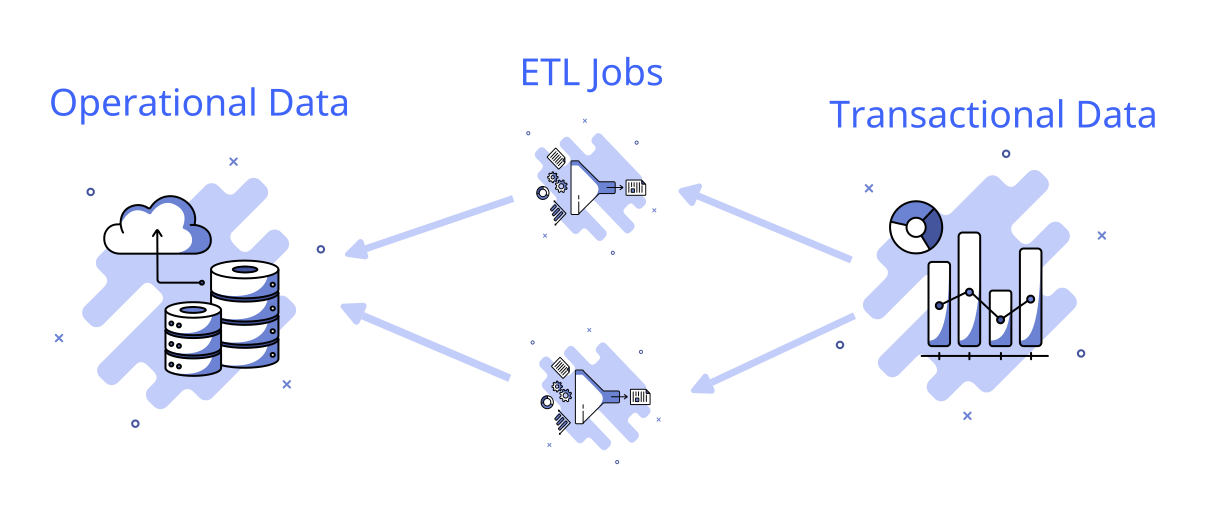
\includegraphics[width=\linewidth]{images/data-planes.png}

  \caption{The great divide of data}

  \label{fig:dataPlanes}

\end{figure}

Many technologies developed over the years are based on this notion. Although these technologies excel in managing the amount, speed, and diversity of data, current data difficulties revolve around the increase in data sources, data quality, and data architecture. 

Information is typically gathered and unified across multiple platforms. Some of this data may exceed the boundaries of the organisation. Therefore, considering the points mentioned earlier and the difficulties outlined, it is suggested that modern data architectures should move away from centralising data in a single large analytical database and instead focus on connecting analytical data from various sources \cite{ataei2022state,DataMesh}. 

The artefact created for this study utilises earlier solutions to improve and overcome their limitations. This artefact tries to move away from highly centralised and rigid data architectures that serve as a bottleneck for coordination. This artefact aims to connect the point of data generation with its utilisation, streamlining the process. This artefact is designed to enhance agility in response to growth and successfully adapt to organisational changes. To achieve that, the first step is the introduction of data into domains. 

\subsection{Localized autonomy through domain-driven design}

Modern enterprises are facing significant complexity. A typical business consists of diverse domains with distinct structures. These domains exhibit varying rates of change and are typically segregated from one another. The business's overall synergy is determined by the relationships and evolution of various domains. 

The core of these synergies is characterised by volatility, frequent market changes, and a growing number of rules \cite{popovivc2018impact}. How do modern organisations handle the effects of these developments on their data? Should they consistently update ETL tasks, develop new ETL pipelines, and merge data into operational repositories? How can firms generate reliable and high-quality data efficiently? It comes down to accepting the change in the current data environment. 

To address this complexity, one approach is to synchronise technology with business objectives. Businesses divide their challenge into smaller components within each domain, integrating technology and data into these areas. This method is well recognised in microservices architectures (Ataei, 2023). 

Central to Terramycelium is the dispersal and decentralisation of services into distinct areas with well-defined boundaries. One of the most difficult aspects of designing a distributed system is determining the architectural quanta on which the system should be divided. This matter has been frequently deliberated among proponents of microservices architecture \cite{merson2020modeling}.Terramycelium, influenced by the works of Eric Evans \cite{evans2004domain} and Dehghani \cite{DataMesh} places data in close proximity to the product domain it pertains to. This suggests that data is within the product domain and is a component of it.

Most businesses nowadays are structured around their products, which is the fundamental driving force behind this approach. These products represent the business's capacity and are divided into different domains. These domains often establish their defined scope, progress at varying speeds, and are managed by interdisciplinary teams \cite{teamtopologiesSkelton}. Integrating data into these specific domains can provide a synergistic effect that enhances the handling of ongoing changes. That is, if data engineering becomes a facet of these products, then there is no need for the sycnrhonization tax that is introduced between operational and analytical systems.

Communication can occur on a micro level between application developers and data engineers over a type definition change in a GraphQL node or on a macro level when application developers consider rebuilding their Protobuff schema in a way that impacts downstream analytical services. Thus, this study integrates the concept of DDD to enhance communication and improve the acceptance, precision, and significance of Terramycelium.

DDD is a software development methodology that emphasises comprehending and representing the problem domain of a software application. The objective of DDD is to develop software that mirrors the language, concepts, and behaviours of the problem domain, prioritising these aspects over technical factors. 

DDD can assist Terramycelium by offering a structured method for modelling and handling data that is well-matched with the application's issue domain. DDD can assist data architects in obtaining a more profound comprehension of the necessary data and its structure by concentrating on the language, concepts, and behaviours of the problem domain \cite{DataMesh}. Effective communication is crucial in software development projects, as it facilitates the sharing of vital knowledge \cite{sudhakar2012model}. 

Data engineers and business stakeholders frequently do not connect directly. Domain knowledge is conveyed through intermediaries like business analysts or project managers into a set of activities to be completed \cite{khrononov2021learning}. This indicates the need for at least two translations from two distinct ontologies.

Each translation results in the loss of crucial subject expertise, posing a danger to the overall data quality. During a data engineering process, the requirements can become twisted, and the data engineer may lack awareness of the specific business domain or problem being addressed \cite{khononov2021learning}.

Data engineering challenges are typically complex and wide-ranging, rather than simple mathematics problems or puzzles. An organisation may choose to enhance workflows and processes by consistently making decisions based on data. However, a rigid and inflexible centralised data architecture can increase the likelihood of project failure. After having the problem broken down to domains, we have to apply some system thinking, that is, should the data centralization break into different data domains, how do we ensure that these domains are healthy and evolving? This is where the concepts of complex adaptive systems are applied.

\subsection{Complex adaptive systems}

Terramycelium architectures have characteristics similar to those of complex adaptive systems (Holland, 1992). The artefact created for this study is inspired by the concept that powerful groups might form based on basic rules that control individual agents. For instance, Reynolds \cite{reynolds1987flocks} examined a coordinated group of starling birds during the autumn season. The study revealed that each starling bird adheres to three basic rules: alignment, separation, and cohesion. The rules can be mathematically articulated as follows:

Alignment:

$$ v_i(t+1) = v_i(t) + \frac{1}{k} \sum_{j=1}^{N} (v_j(t) - v_i(t)) $$

where $v_i(t)$ is the velocity vector of bird $i$ at time $t$, $k$ is a normalization factor, and $N$ is the number of neighbouring birds.

Cohesion:

$$ v_i(t+1) = v_i(t) + \frac{1}{k} (c_i(t) - p_i(t)) $$

where $c_i(t)$ is the center of mass of the neighbouring birds, $p_i(t)$ is the position of bird $i$ at time $t$, and $k$ is a normalization factor.

Separation:

$$ v_i(t+1) = v_i(t) + \sum_{j=1}^{N} \frac{(p_i(t) - p_j(t))}{d_{ij}^2} $$

where $p_i(t)$ is the position of bird $i$ at time $t$, $p_j(t)$ is the position of bird $j$ at time $t$, and $d_{ij}$ is the distance between birds $i$ and $j$.

Starling birds do not require a centralised orchestrator to form this intricate adaptive system. Terramycelium aims to encourage a domain-driven allocation of data ownership. This architecture is designed to offer not just operational data but also analytical data through a standard interface. For instance, the practice management software for veterinarians includes operational APIs for updating animal attributes and analytical interfaces for retrieving animal data within a specific time frame. Each domain owns its own data.

The domain can retrieve data from other domains using a discovery mechanism, process the data, and augment its own data. Aggregate domains are created to collect data from different domains and make it available for a certain purpose. 

This aims to eliminate vertical dependency and enable teams to have local autonomy while being equipped with the appropriate amount of discovery and APIs. This architecture emphasises the concept of coequal nodes working together to accomplish the system's overarching objective, rather than relying on a centralised database managed by individuals lacking domain expertise. This idea is influenced by DDD as described by Evans \cite{evans2004domain}, Data Mesh by Dehghani \cite{DataMesh}, microservices architecture by Newman \cite{newman2021building} and Complext Adaptive systems by Lansing \cite{lansing2003complex}. 

\subsection{Event driven services}

Terramycelium's decentralised and distributed structure poses difficulties in service communication as the network expands. At first, basic point-to-point communication via REST API calls is adequate, but it becomes inefficient as the system grows. Synchronous interactions can result in a `distribution tax', where one service's blocked state, generally caused by costly procedures, leads to delays in dependent services \cite{montesi2016circuit}.

Distributed systems' extensive network requirements can lead to complications such as tail latency, context switching, and gridlocks. This strong interconnection contradicts the distributed system's objectives of independence and robustness.

Terramycelium uses asynchronous, event-driven communication to address these concerns. This approach allows services to publish and respond to events, separating their interactions. Within the `publish and forget' paradigm, services broadcast events to designated topics and proceed without waiting for immediate reactions.

Event-driven architectures usually provide eventual consistency, which may not be ideal for some real-time stream processing situations. However, it is generally safe to assume that most data engineering tasks can effectively function within an event-driven framework.

As per Ford et al. \cite{Ford2021SoftwareArchitecture}, event-driven architectures consist of two primary topologies: 1) broker topology and 2) mediator topology. The concept of streaming platforms is further explained in the writings of Stopford \cite{stopford2018designing}. Terramycelium, as a BD architecture designed for processing analytical data, eliminates several issues associated with accomplishing ACID transactions. Terramycelium utilises the architectural principles of distributed, asynchronous, event-driven systems with a mixed topology. Terramycelium is incorporating aspects of broker topology, mediator topology, and several notions from streaming platforms. Terramycelium's CAP theorem \cite{simon2000brewer} prioritises partition tolerance and availability as key assurances. 

Terramycelium's hybrid topology consists of five main architectural components: the event, the event consumer, the event producer, the event backbone, and the eventing interface. Events are triggered by the event producer and sent to the relevant topic through the eventing interface. The event is processed by the event broker and stored in a queue-like indexed data structure for later retrieval inside the event backbone. Interested event consumers will listen to the topic of interest using the eventing interface. The event backbone is an internally distributed system composed of numerous event brokers. 

Event brokers are services created and provided to enable event communication via Terramycelium. The brokers are synchronised with a decentralised service coordinator. Brokers also enable the replication of topics. Additionally, the event backbone includes a specialised event archive to ensure fault tolerance and recoverability. The purpose of this archive is to retain all events processed by the brokers for potential restoration in the event of a failure. 

These components collaborate to establish a distributed, fault-tolerant, and scalable data system capable of managing both batch and stream processing, as seen in Figure \ref{fig:eventDrivenArchitecture}. 

\begin{figure*}[ht]

  \centering

  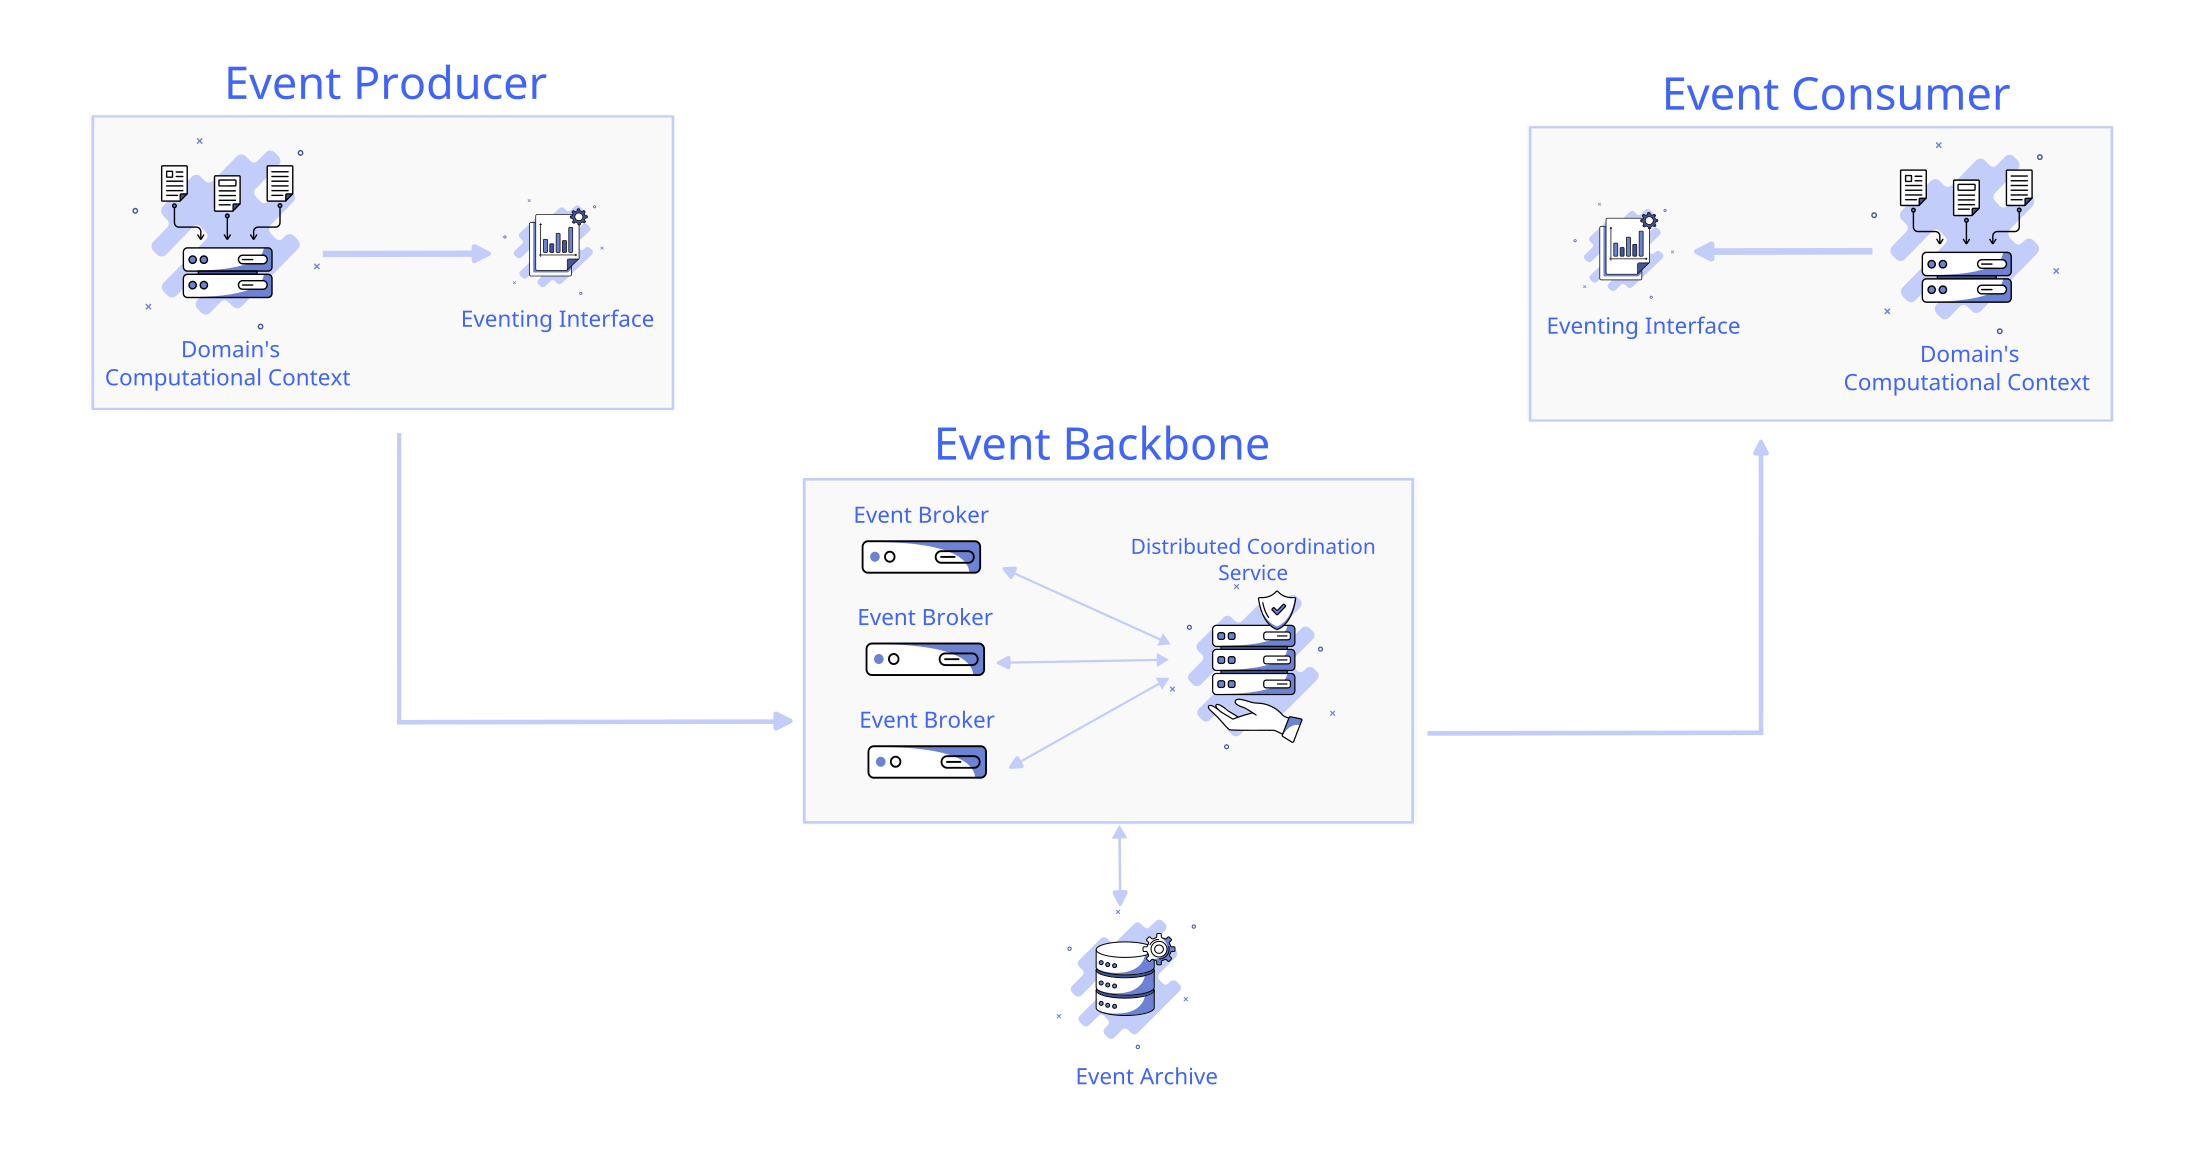
\includegraphics[width=13cm]{images/Event-architecture.png}

  \caption{Terramycelium Event-driven Architecture}

  \label{fig:eventDrivenArchitecture}

\end{figure*}

\subsection{Architectural characteristics}

After discussing the main design theories that underpin Terramycelium, in this section, the overall architectural characteristics of this artefact are discussed. The Terramycelium architecture is distinguished by its emphasis on maintainability, scalability, fault tolerance, elasticity, and deployability. It is in line with contemporary engineering methodologies like automated deployment and continuous integration \cite{Ford2021SoftwareArchitecture}. The architecture focuses on utilising microservices, which are autonomous components that can be deployed and maintained separately.

This architecture emphasises improved maintainability in comparison to current data architectures. Event-driven microservices architecture enables modular development and independent scaling, facilitating the maintenance and updating of individual components without impacting the entire system. The design also enables automated deployment processes, which help streamline upgrades and minimise manual interaction.



Scalability and elasticity are significant aspects as well. The architecture allows for horizontal scalability, enabling the addition or removal of services according to demand. This adaptability guarantees that the system can efficiently manage different workloads.

The architecture also demonstrates strong fault tolerance. Interservice communication can affect fault tolerance; however, a redundant and scalable design of Terramycelium, combined with service discovery techniques, helps alleviate this problem. Microservices' standalone and single-purpose design typically results in a high level of fault tolerance \cite{MStodaytomorrow}.

On the other hand, the architecture might be rated lower in terms of cost and simplicity. The decentralised structure of Terramycelium and the possibility of higher communication overhead can create challenges in cost management and optimisation. Implementing strategies like intelligent data caching and replication can help overcome performance issues related to network calls, but managing costs is still a continuous concern.

The Terramycelium design emphasises the advantages of microservices, focusing on maintainability, scalability, fault tolerance, elasticity, and deployability. The text recognises the difficulties that come with distributed architectures and provides methods to reduce their impact. Architects need to comprehend the principles of architecture in order to skillfully traverse and capitalise on its advantages. An overview of architectural characteristics is portrayed in Table~\ref{tab:architecture-characteristics}

\begin{table}[t]

  \centering

  \caption{Terramycelium Architecture Characteristics}

  \label{tab:architecture-characteristics}

  \begin{tabular}{|l|c|}

    \hline

    \textbf{Characteristic} & \textbf{Score} \\

    \hline

    Maintainability & $\bigstar\bigstar\bigstar$ \\

    \hline

    Scalability & $\bigstar\bigstar\bigstar\bigstar$ \\

    \hline

    Fault Tolerance & $\bigstar\bigstar\bigstar$ \\

    \hline

    Elasticity & $\bigstar\bigstar\bigstar\bigstar$ \\

    \hline

    Deployability & $\bigstar\bigstar\bigstar\bigstar$ \\

    \hline

    Cost & $\bigstar\bigstar$ \\

    \hline

    Simplicity & $\bigstar$ \\

    \hline

    Performance & $\bigstar\bigstar\bigstar$ \\

    \hline

    Support for Modern Engineering Practices & $\bigstar\bigstar\bigstar\bigstar$ \\

    \hline

  \end{tabular}

\end{table}

\section{Artifact} \label{sec:artefact}

After exploring the underpinning design theories, a solid theoretical foundation is established for creating and developing the artefact. Terramycelium is generated using Archimate and mostly showcases the RA within the technological layer. The architect has the responsibility to determine the flow and application that should be present in each node when showcasing these services in the technology layer. To ensure thoroughness, a basic business process is assumed, as every piece of software is created to fulfil a business requirement. Terramycelium should possess the flexibility needed to accommodate alternative business models, notwithstanding potential variations in the business layer across different settings.

This BD RA does not depict the architecture of any particular BD system. It functions as a versatile tool for describing, discussing, and constructing system-specific designs based on standardised principles. Terramycelium enables in-depth and insightful talks about the needs, frameworks, and functions of BD systems. The system stays vendor-neutral, providing flexibility in choosing products or services, and avoids imposing strict solutions that restrict innovation. 

To ensure thoroughness, we have assumed a basic BD business process, as all software is created to fulfil a specific business requirement. Terramycelium consists of 15 primary components and 5 variable components, as seen in Figure \ref{fig:Terramycelium}. The lowercase "a" in the top left corner of the diagram represents the auxiliary view, while the letter "m" represents the master view. When the same entity is utilised in various models, the auxiliary view is employed. This indicates that the entity already exists and is being reused. 

\begin{sidewaysfigure*}

  \centering

  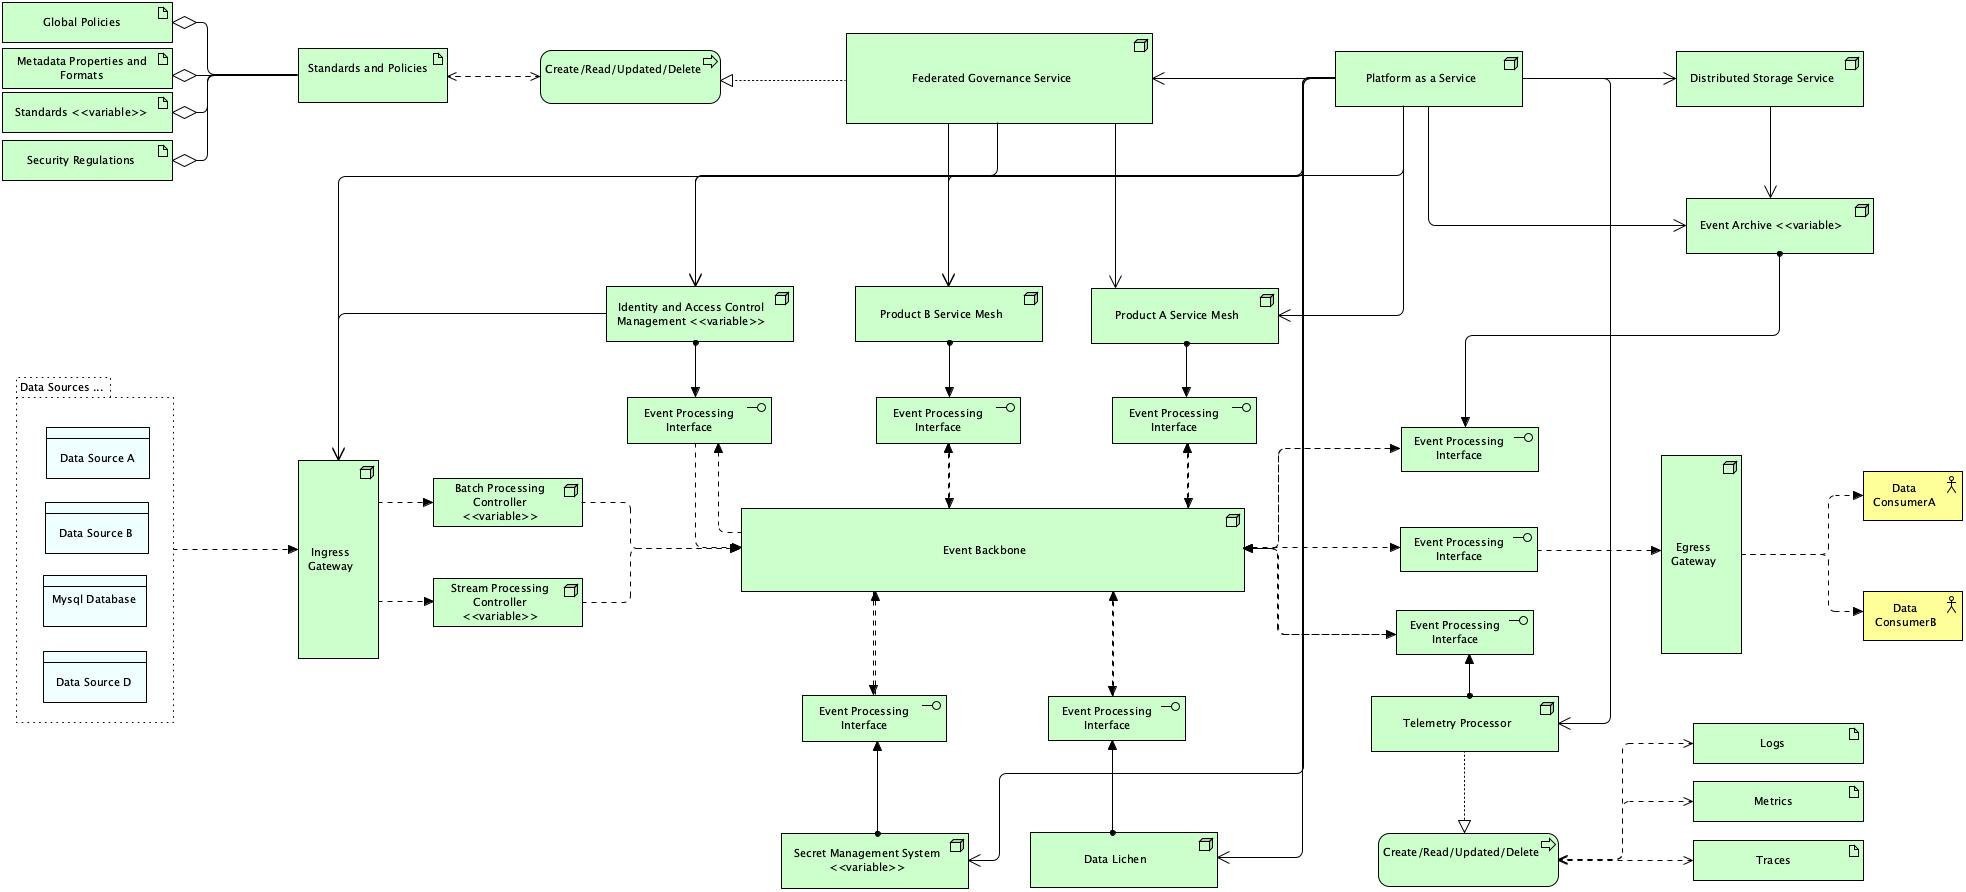
\includegraphics[width=\textwidth]{images/Metamycelium.jpg}

  \caption{Terramycelium}

  \label{fig:Terramycelium}

\end{sidewaysfigure*}

While this business layer could vary in different contexts, Terramycelium should be able to have the elasticity required to account for various business models. To ease understanding of the RA, we sub-diagrammed the product domain in Figure \ref{fig:TerramyceliumServiceMesh}.

\begin{figure*}

  \centering

  \includegraphics[width=\textwidth]{images/MetamyceliumServiceMesh.jpg}

  \caption{Service Mesh}

  \label{fig:TerramyceliumServiceMesh}

\end{figure*}

These components are;

\begin{enumerate}

    \item \textbf{Ingress Gateway:} The ingress gateway is pivotal in Terramycelium, acting as the main entry point for external requests. It exposes necessary ports and endpoints, intelligently load-balancing traffic to the appropriate processing controllers, thereby enhancing the system's scalability and performance.

    Security is significantly bolstered by the ingress gateway, which prevents direct service access by centralising entry and enabling the enforcement of security policies such as SSL termination and authentication. This approach secures communication with external entities and streamlines SSL processing, offloading this task from downstream services.

    

    The gateway also allows for incoming data modification or enrichment, offering customisation and system integration capabilities. This architectural component simplifies monitoring and observability, concentrating metrics, logging, and tracing at a singular point for efficient analysis and compliance oversight. Additionally, it supports network segmentation, establishing a clear demarcation between public interfaces and private network resources, thus reinforcing security and control over data flow.

    

    \textit{Addresses requirements: Vol-1, Vol-2, Var-1, Var-3, Var-4, Val-1, Val-3, Val-4, SaP-1, and SaP-2.}

    \item \textbf{Batch Processing Controller:} The primary function of the batch processing controller is to manage batch events by sending them to the event backbone. The dedicated service, which may be a tiny service or a Lambda function, processes batch-processing requests and converts them into events for the event broker. Its unique characteristics enable it to handle batch requests in large quantities and asynchronously, distinguishing it from stream processing controllers.

    The batch-processing controller offers various architectural advantages. Firstly, it greatly improves monitoring capabilities, offering clearer insight into the status and performance of batch activities. This efficient monitoring simplifies problem-solving and performance evaluation, guaranteeing that batch processing adheres to defined criteria and performance standards.

    

    The batch processing controller allows for customisation and flexibility in generating batch events. It can carry out supplementary functions apart from computationally demanding activities, including data cleansing or incorporating personalised headers. Businesses can customise batch event production to meet their individual needs and expectations.

    

    A specialised controller for batch processing recognises the distinct needs and attributes of batch events, offering tailored features and enhancements. This component fulfils the criteria.

    \textit{Addresses requirements: Vel-1, Val-1, and Val-2.}

    

    \item \textbf{Stream Processing Controller:}  The stream processing controller is a crucial component in architecture, handling streaming events and dispatching them to the event backbone. It is distinct from batch processing services as it focuses on non-heavy computations optimized for stream processing requirements. It can enable stream provenance, providing insights for data governance and traceability. It can also leverage one-pass algorithms for stream analytics tasks.

    A dedicated stream processing controller allows for the association of custom attributes with stream events, enabling contextual enrichment of streaming data and differentiated treatment based on the system's nature. This enables real-time decision-making or targeted actions based on event content.

    

    Simplifying monitoring and discovery within the architecture, the controller simplifies tracking and analysing the performance, latency, and throughput of streaming events. It also enables focused monitoring of stream-specific metrics, providing valuable insights into the behaviour and efficiency of the streaming data pipeline.

    

    In summary, the stream processing controller is an essential component in architectures involving streaming data due to its ability to handle high throughput, apply custom attributes, optimise computations, and simplify monitoring and discovery. 

    

    \textit{Addresses requirements: Vol-1, Vel-1, Vel-2, Vel-4, Vel-5, and Val-2.}

    

    \item \textbf{Event Processing Interface:} Event brokers are designed to achieve \emph{inversion of control}. As the company evolves and requirements emerge, the number of nodes or services increases, new regions of operations may be added, and new events might need to be dispatched. As each service has to communicate with the rest through the event backbone, each service will be required to implement its event-handling module. 

    

    This can easily turn into a spaghetti of incompatible implementations by various teams, and can even cause bugs and unexpected behaviours. To overcome this challenge, an event broker is introduced to each service of the architecture. Each service connects to its local event broker and publishes and subscribes to events through that broker. One of the key success criteria of the event broker is a unified interface that sits at the right level of abstraction to account for all services in the architecture. 

    

    Event brokers, being environmentally agnostic, can be deployed on any on-premise, private, or public infrastructure. This frees up engineers from having to think about the event interface they have to implement and how it should behave. Event brokers can also account for more dynamism by learning which events should be routed to which consumer applications. Moreover, event brokers do also implement circuit breaking, which means if the service they have to break to is not available and does not respond for a certain amount of time, the broker establishes the unavailability of the service to the rest of the services, so no further requests come through. This is essential to preventing a ripple effect over the whole system if one system fails. 

    

    \textit{Addresses requirements: Val-1, Ver-1.} 

    \item \textbf{Event Backbone:} The event backbone is the central component of the Terramycelium, enabling communication between nodes. Distribution and clustering should be implemented to handle the system's scalability. Communication is orchestrated by coordinated activities, like a dance ensemble. Every service monitors and responds to the event backbone, performing the required actions. 

    

    This guarantees an uninterrupted exchange of data between services, ensuring that all systems are in the appropriate condition. The event backbone can combine many event streams, store events in a cache, archive events, and perform other operations, as long as it does not become overly intelligent or function as an Enterprise Service Bus (ESB) in Service-Oriented Architecture (SOA) systems. An architect should see the event backbone as a collection of interconnected nodes that address different subjects of interest. The event backbone can be monitored over time to analyse access patterns and adjusted to optimise communication efficiency.

    \textit{Addresses requirements: Vel-1, Vel-2, Vel-3, Vel-4, Vel-5, Val-1, Val-2, Ver-1, Ver-2, and Ver-3.} 

    

    \item \textbf{Egress Gateway:} The inclusion of an egress gateway in Terramycelium offers numerous advantages, especially for external data consumers. In this architecture, data consumers first interact with the discovery component, known as Data Lichen, which serves as a central hub for accessing available data domains. Once connected to Data Lichen, data consumers can navigate to the relevant data domain to retrieve the desired data.

    Furthermore, all external data consumers in the system go through a centralised secret management and centralised authentication and authorization component. This centralised approach brings several benefits to the architecture. Firstly, it ensures a consistent and secure management of secrets, such as API keys, access tokens, or credentials, which are essential for data access and security. This centralised secret management enhances the overall system's security posture by reducing the chances of vulnerabilities or misconfigurations in secret handling.

    Secondly, the centralised authentication and authorization component streamlines the authentication and access control processes for external data consumers. By enforcing a unified authentication mechanism, it ensures that all users are properly authenticated and authorised before accessing the system's data resources. This centralised approach simplifies the management of user access rights, improves security, and provides granular control over data access permissions.

    Thirdly, the centralised components simplify the maintenance and scalability of the system. With a single point for managing secrets, authentication, and authorization, it becomes easier to update, monitor, and audit these components. Additionally, this architectural pattern allows for easier scaling and expansion as new data domains or data sources can be seamlessly integrated into the system with consistent authentication and authorization mechanisms.

    Overall, the inclusion of an egress gateway in Terramycelium offers a robust and efficient approach for external data consumers. It ensures standardised data access, enhances security, simplifies maintenance, and enables scalability, making it a highly favourable and beneficial architectural design. 

    

    \textit{Addresses requirements: Vel-2, Vel-4, Val-3, Val-4, SaP-1, and SaP-2.} 

    

    \item \textbf{Product Domain Service Mesh:} Integrating a service mesh as a core element of each product's domain is an effective strategy in the architectural framework. The service mesh consists of essential components that work together to facilitate effective data processing, storage, governance, and communication within the domain. The components consist of batch and streaming data input, analytical and operational services specific to the domain, API access to distributed storage services, an infrastructure API for platform-as-a-service modules, containers hosting the analytical service, a control tower, and integration with a federated governance service's API for policy enforcement using sidecars.

    The service mesh's effectiveness is derived from its architectural design and its capability to meet essential needs. By integrating the domain's functionalities into a service mesh, the interdependence across teams is removed, enabling greater team independence. The components of the service mesh collaborate to provide benefits like data ingestion into the analytical service domain, API connectivity to distributed storage services, container hosting for the analytical service domain, a control tower, and integration with a federated governance service's API for policy enforcement using sidecars.

    

    The service mesh architecture provides the analytical service with direct access to operational data, connecting data analytics and operational systems. The analytical service can obtain real-time insights and a comprehensive overview of the system's activities, which minimises the requirement for manual data extraction and transformation procedures. Accessing operational data directly improves the efficiency and precision of analytical services, leading to more precise analysis and well-informed decision-making.

    

    The service mesh architecture enables a cohesive perspective of the system, promoting smooth cooperation between analytics and operations teams. The system supports scalability, adapts to changes in business environments, validates data, maintains quality and integrity, and meets security and privacy standards by enforcing policies, ensuring secure communication, and implementing data governance processes.

    The service mesh's effectiveness lies in its ability to address key architectural concerns. It promotes scalability, allowing the domain to handle large volumes of data and increasing computational resources as needed (Vol-1). It facilitates rapid development and deployment of analytical capabilities (Vel-3, Vel-4, Vel-5). The service mesh architecture accommodates variability in business contexts, supporting the diverse needs and requirements of different product domains (Var-1, Var-2, Var-3). It ensures data validation, quality, and integrity by leveraging advanced analytics and processing techniques (Val-1, Val-2, Val-3, Val-4). Security and privacy requirements are fulfilled through policy enforcement, secure communication, and data governance mechanisms (Sap-1, SaP-2). 

    

    Finally, the service mesh architecture allows for the verification of system behaviour, enabling efficient testing, monitoring, and verification of the domain's analytical outputs (Ver-1, Ver-2, Ver-3).

    \textit{Addresses requirements: Vol-1, Vel-3, Vel-4, Vel-5, Var-1, Var-2, Var-3, Val-1, Val-2, Val-3, Val-4, Sap-1, SaP-2} 

  

    \item  \textbf{Federated Governance Service:} Terramycelium's distributed architecture comprises multiple independent services with distinct lifecycles, developed and deployed by autonomous teams. To ensure coherence and prevent interface conflicts without centralising control, global federated governance is essential. This governance model standardises services, enhances their interoperability, and facilitates team collaboration. It also mitigates risks, such as non-compliance with GDPR, by establishing a unified framework of global policies, metadata standards, API standards, and security protocols. This framework not only supports organisational practices but also aligns with external regulations, safeguarding against potential fines and security threats. The federated governance service, comprising components like global policies, metadata standards, and security regulations, plays a pivotal role in maintaining the architecture's integrity and adaptability, indirectly impacting all requirements. This component can indirectly affect all requirements.

    \textit{Addresses requirements: All.}     

    \item \textbf{Data Lichen:} With an increasing number of products, more data is accessible for users, leading to enhanced interoperability but also posing greater challenges for maintenance. Without an automated method for different teams to obtain their desired data, a tightly connected and sluggish data culture would develop. To overcome these obstacles and enhance the ability to find, work together, and navigate with guidance, the Data Lichen should be put into practice. Gartner has identified data discovery mechanisms such as Data Lichen as essential tools. These mechanisms facilitate improved communication dynamics, quicker data access through services, and intelligent collaboration among services.

    \textit{Addresses requirements: Vel-4, Var-1, Var-3, and Var-4.} 

    

    

    \item \textbf{Telemetry Processor:}  The decentralised architecture of Terramycelium poses challenges for debugging, fault identification, and maintenance as it requires tracking transactions across several services. Consolidating the handling of telemetry data in Terramycelium provides architectural advantages by streamlining data processing, offering a cohesive perspective of logs, metrics, and traces, facilitating thorough analysis and correlation, and guaranteeing optimal resource distribution. Centralising the service guarantees uniform monitoring and governance processes throughout the architecture, encouraging compliance with best practices.

    The centralised service can act as a data source for different users, like the Data Lichen, which uses processed telemetry data to create important insights. This service may process data that can be used by customised systems and dashboards, offering adaptability and scalability to fulfil particular business needs. This promotes a data-driven environment, enabling individuals to get valuable information and insights from the analysed telemetry data. The flexibility and ease of access to the telemetry data increase the benefits of the centralised service in the larger BD framework.

    \textit{Addresses requirements: Vol-1, Vel-1, Val-1, and Ver-1.} 

    \item \textbf{Event Archive:} As the quantity of services expands, the subjects in the event backbone rise, leading to a surge in the number of events. If such circumstances occur, there is a possibility of failure leading to a timeout and subsequent loss of a sequence of events. This can lead to the system being in an incorrect state, causing a harmful chain reaction that affects all services. Terramycelium often addresses these issues by utilising an event archive. The event archive is in charge of recording occurrences for future retrieval in case of failure. 

    

    During a blackout in a specific area, if the event backbone is down, it can restore itself and return the system to its correct state by retrieving events from the event archive. The event interface manages circuit breaking to prevent services from sending additional requests to the backbone while it is not functioning. The determination of the duration till expiration and the selection of events to be stored are made according to the specific circumstances in which Terramycelium is utilised.

    \textit{Addresses requirements: Vol-1, Vel-1, Val-1, and Ver-1.} 

    \item \textbf{Distributed Storage Service:} Terramycelium supports decentralised and distributed systems but does not require each product domain to have its own unique data store. To avoid duplication, conflicting data storage methods, reduced interoperability across services, and absence of consistent data storage techniques, The distributed storage service is intended to store vast amounts of data in its original format until it is ready to be retrieved for analysis and other uses. 

    

    Data can be stored in the distributed storage service with the appropriate domain ownership before being accessed and used by different services. Data of various structures, such as structured, semi-structured, unstructured, and pseudo-structured, can be stored in a distributed storage service before being processed in batches or streams. However, not all data should be sent straight to this service; the data flow depends on the specific context in which the system operates.

    

    \textit{Addresses requirements: Vol-2, Vel-1, Var-1, Var-3, Var-4, Val-3.} 

    \item \textbf{Platform as a Service:} The Platform as a Service (Paas) component acts as a central hub, providing an API to all other system components. This PaaS component is essential for facilitating the independence and expandability of the entire infrastructure.

    The primary design value of this PaaS component is its capacity to simplify the underlying infrastructure difficulties. By offering a standardised API, each component can autonomously handle and allocate necessary resources like computing power, storage, and networking without having to deal with the complex specifics of the underlying infrastructure. This abstraction layer encourages a minimal connection between components, making it simpler to create, deploy, and maintain the entire system.

    

    The PaaS component places importance on scalability and elasticity as key design values. It allows for the flexible allocation and deallocation of resources according to the changing requirements of diverse data domains. The PaaS component facilitates effective infrastructure utilisation by providing an API that allows components to request resources as required. The system may adjust resources as needed to maintain peak performance and cost efficiency throughout the whole architecture.

    

    Data domains can utilise the PaaS API to request, set up, and oversee resources, allowing them to function autonomously and effectively. Decentralising infrastructure management improves agility and flexibility in the system.

    

    \textit{Addresses requirements: SaP-1, SaP-2, Var-1, Var-3, Var-4, Vel-1, and Vol-2.} 

    \item \textbf{Identity and Access Management:} The role of the Identity and Access Management (IAM) component is to guarantee secure and regulated access to the system's resources and data. The concept includes a range of architectural principles necessary for upholding data integrity, privacy, and regulatory compliance.

    The IAM component places significant emphasis on authentication and authorization as core design concepts. The system offers strong methods to verify the identities of users, components, and services in the structure, guaranteeing that only approved entities can get the resources and carry out particular tasks. These measures aid in preventing unauthorised access, reducing security risks, and protecting sensitive data.

    

    Another architectural value of the IAM component is its emphasis on centralised user and access management. It acts as a centralised authority for overseeing user identities, responsibilities, and permissions throughout Terramycelium. Centralization optimises access control management, speeds user onboarding and offboarding, and maintains uniform security policy enforcement system-wide.

    

    The IAM component guarantees meticulous access control and privilege management, enabling the creation of precise access policies. The system enables strong authentication using standard protocols such as OAuth and SAML, simplifying user access through Single Sign-On (SSO). It supports audits by recording access occurrences, strengthening compliance, security oversight, and incident management. The Figure~\ref{diagram:IAM} provides a detailed representation of how the component functions and how it interacts with other aspects of the system.

    \begin{figure*}[ht]

        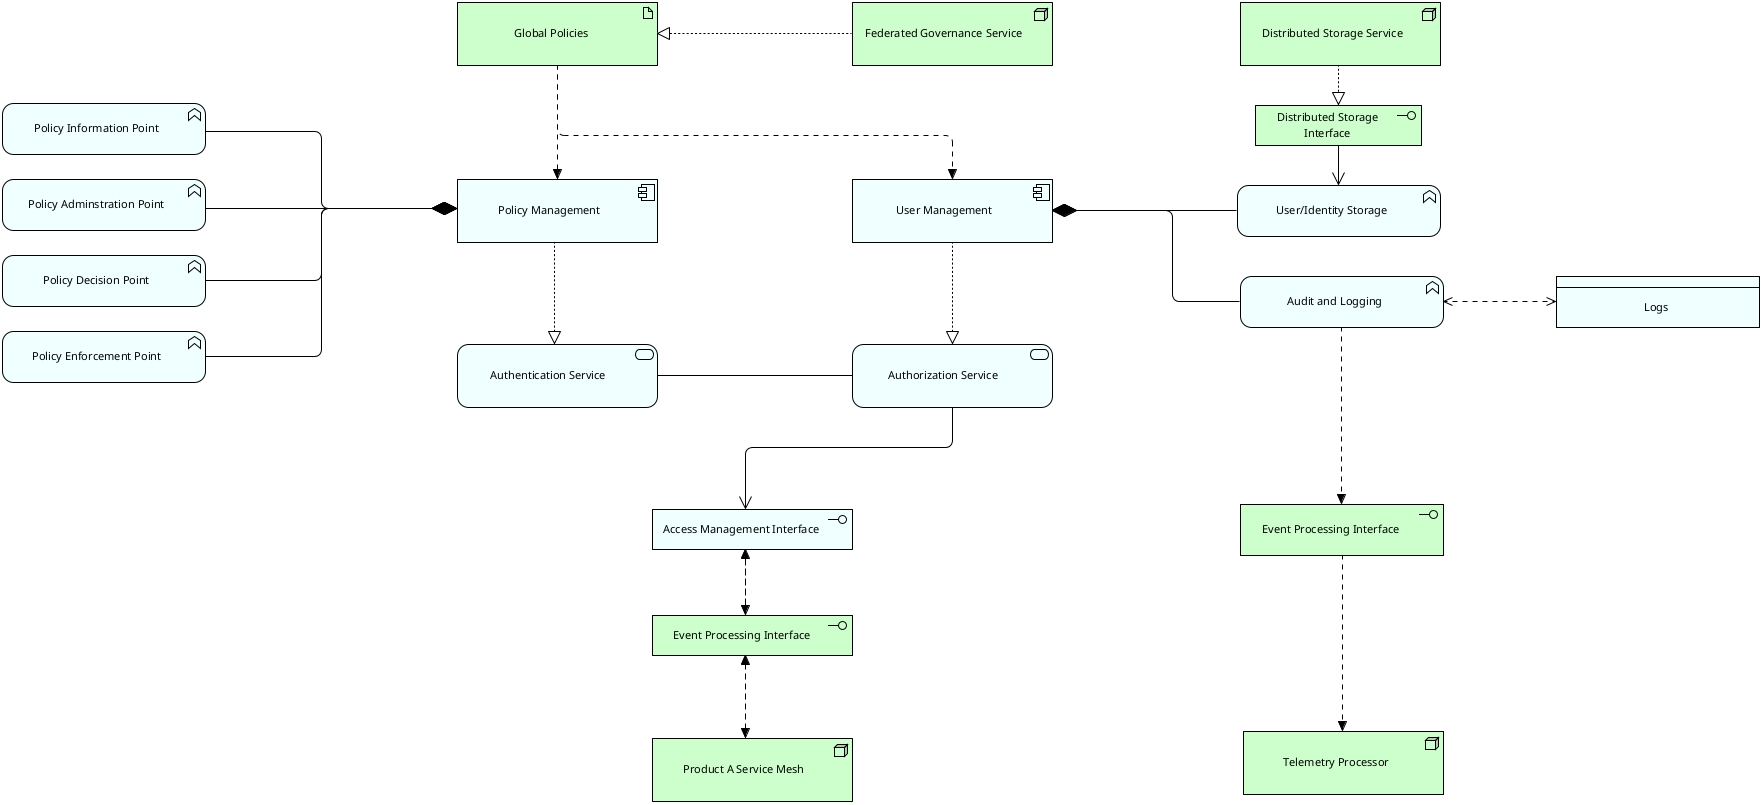
\includegraphics[width=\linewidth]{images/Metamycelium-identity-and-access-control.jpg}

        \caption{Identity and Access Control Management System}

        \label{diagram:IAM}

    \end{figure*}

    \textit{Addresses requirements: SaP-1, and SaP-2.} 

    

    \item \textbf{Secret Management System:} The central secret management system is a crucial component for securely storing and maintaining sensitive information, including passwords, API keys, cryptographic keys, and other secrets.

    

    The central secret management system places a strong emphasis on securely storing and encrypting secrets as a fundamental design principle. The system uses strong encryption algorithms and processes to safeguard sensitive data while it is kept, guaranteeing that confidential information is securely protected and cannot be accessed by unauthorised parties. This value aids in preventing unauthorised access to secrets, reducing the risk of data breaches, and guaranteeing confidentiality.

    

    The secret management system also facilitates the secure distribution and retrieval of secrets to authorised components or services. It offers safe APIs or client libraries that allow secrets to be retrieved securely during runtime. This value ensures that confidential information is only available to authorised entities who need it, preventing the unauthorised disclosure of secrets.

    

    The secret management system also encourages integration with other components and services in Terramycelium. The system offers APIs and integration points that enable smooth integration of secrets into different data domains. This integration value enables authorised components to securely and conveniently access secrets, ensuring operational efficiency and minimising obstacles in development and deployment procedures.

    

    \textit{Addresses requirements: SaP-1, and SaP-2.} 

\end{enumerate}

The variable components in Terramycelium can be altered, adapted, or excluded according to the architect's discretion and the specific characteristics of the situation. This RA aims to enhance data architects' decision-making process by introducing established patterns and best practices from several perspectives, rather than restricting their innovation. Alternative choices for each variable module are not detailed due to the dynamic nature of the industry, and architects strive to create systems that tackle new issue areas. 

\section{Evaluation 1: Case Mechanism Experiment}



The validation of treatment is crucial in its research, development, and implementation phases \cite{wieringa2014design}. Validating a treatment involves determining its possible impact on stakeholder objectives when applied to the specific problem at hand. 

Clearly outlining and justifying the treatment needs establishes a straightforward avenue for validation. This implies that the treatment may be verified by showing that it fulfils certain predetermined criteria. A key challenge in treatment validation is the absence of real-world implementation to assess the treatment's impact on stakeholder objectives. This challenge emphasises the need for thorough, diverse, and well-thought-out assessment methods, as discussed more in the next sections. 

The initial phase of evaluating Terramycelium is a single-case mechanism experiment based on the parameters outlined by Wirienga \cite{wieringa2014design}. Although Wirienga's works reference a single experiment, this study considers a few experiments. A multi-case experiment is required because the artefact is complex, which improves the thoroughness and significance of the evaluation process, leading to a more detailed and nuanced comprehension of the artefact's capabilities and possibilities. 

\subsection{Prototyping an Architecture}

Prototyping is the creation of a working model that physically represents the structure, demonstrating the design principles and ideas. This is frequently referred to as the \emph{concrete architecture}. This technique enables researchers to validate and develop the design to assess its practicality, performance, and alignment with research objectives.

Implementing the essential components and functionalities stated in the RA, Terramycelium, is part of prototyping the architecture. The selected technologies, supported by academic justification and in line with the research goals, serve as the basis for developing the prototype. The architecture's ability to manage large-scale data processing and meet various needs can be evaluated by systematically implementing its architectural components. Figure~\ref{TerramyceliumPrototype} shows a concrete structure created with Terramycelium.

\begin{figure*}[ht]

    \centering

    \includegraphics[width=\linewidth]{images/MetamyceliumConcrete.jpg}

    \caption{Terramycelium Prototype}

    \label{TerramyceliumPrototype}

\end{figure*}

\subsection{Stage 1: Formation}

All components of this prototype are integrated within a single Kubernetes cluster. Therefore, KIND \cite{KIND2023} has been selected as the local Kubernetes cluster for this prototype to function. 

The reproducibility of this technique is crucial. The scripts required to execute, download, and set up artefacts are located in the scripts folder of the Github repository, cited as \cite{terramyceliumInfrastructure}. These scripts are designed to exclusively operate on Unix-like operating systems.

After establishing the fundamental scripts for initialising the cluster, the procedure commenced with the creation of various services within the Kubernetes cluster. Helm Charts from Artefact Hub \cite{ArtifactHub2023} are utilised for enhanced maintainability and scalability of Nginx ingress and Kafka. Terraform was subsequently used to implement the charts on the Kubernetes cluster. It is located in the IaaC folder of the repository. 

We conducted an extensive search for helm charts for all artefact components and selected a mature and well respected chart from Bitnami for Nginx. Using this method is favoured over developing unique directives for Nginx ingress in Kubernetes and linking services to each other through Kubernetes architectural elements such as Services or StatefulSets.

After this, a search has been done for other charts for other components of the concrete architecture on Artefact Hub. After selecting an appropriate chart for Nginx ingress, Keycloak, and Vault, the telemetry processor service is created. 

Initially, a FastAPI app is set up. The programme is containerised using Docker, hosted on Github sites, and integrated into Terraform Helm release resources for deployment on the local KIND cluster. The Kubernetes ingress controller is configured as Nginx and deployed to the local cluster using Terraform. 

Once the ingress controller is established, the ingress resources are configured to direct traffic to Kafka-rest-proxy. The Kafka-rest proxy is included in the artefact to simplify data access from the cluster. Kafka uses the binary protocol instead of HTTP, whereas most services depend on HTTP for network connections. 

Upon successful configuration of the Nginx ingress and Kafka REST proxy, Keycloak is installed and seamlessly integrated into various components of the architecture. The Vault is incorporated into the cluster using HashiCorp's official helm chart \cite{HashiCorpVaultHelm2023}. 

Next, the major system to be implemented is Data Lichen. Data Lichen required a new frontend to be developed from scratch. A template engine for Node.js called EJS was chosen for this purpose. This template engine was selected for its ability to simplify development and speed up the operations of this trial. 

The goal is to create a simple user interface for Data Lichen that successfully showcases the framework's potential design and capability, rather than building a comprehensive frontend. Various teams may opt to adopt Data Lichen in diverse ways. Data Lichen must be developed from scratch because there is no existing open-source technology that offers the necessary features.

Once Data Lichen has been organised and implemented in the cluster, an Istio service mesh is established. To achieve this goal, various Kubernetes namespaces are established, and various services are categorised within the same namespace for the service mesh to manage and function. Istio's Kiali dashboard is implemented to enhance the development experience and observability. 

Minio's chart is installed, and the dashboard is active. The last component that needed to be deployed was Open Policy Agent (OPA). There are multiple methods to incorporate OPA into an architecture. This can be accomplished via a solo Envoy proxy, a Kubernetes operator, a load balancer with Gloo Edge, or through Istio. 

Istio was chosen because it has already been selected and deployed on the cluster. Nevertheless, automatically injecting policies into services inside a particular service mesh is a complex operation. This was done by extending the Envoy sidecar with an external authorizer API to implement inbound and outbound policies. 

OPA is incorporated into the service mesh as an independent service known as a sidecar proxy. The OPA functions as an admission controller, evaluating requests sent to the Kubernetes API server. 

OPA assesses these requests based on established policy guidelines. Approved requests are executed by the API server, whereas refused requests result in an error message sent to the user. OPA's policies manage all interactions among services and pods within a namespace. OPA assists in ensuring adherence to predetermined security and operational regulations within a Kubernetes setting. This is depicted in Figure~\ref{OPAISTIO}.

\begin{figure*}[ht]

  \centering

  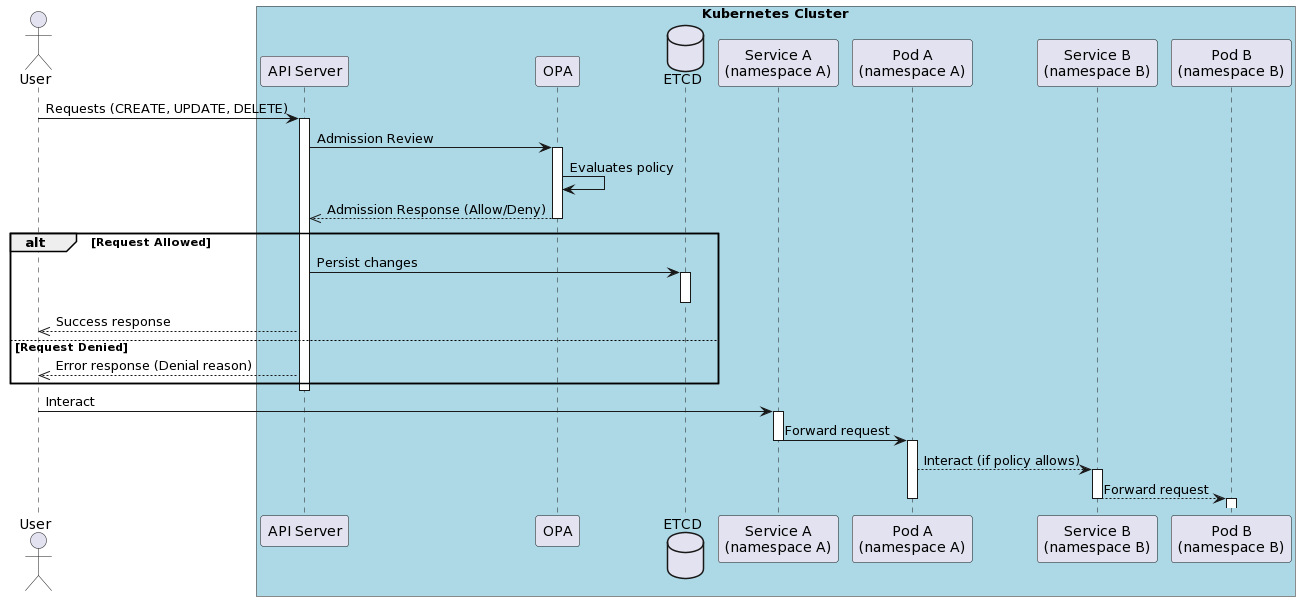
\includegraphics[width=\linewidth]{images/OPA-istio-flow.png}

  \caption{Open Policy Agent Communication Flow with Other Services}

  \label{OPAISTIO}

\end{figure*}

Once OPA was implemented, the analytics service for the domain was created using the Python framework FastAPI. To meet the requirements of Terramycelium, a domain incorporating operational and analytical systems must be established. Since this experiment is not a genuine business, it is logical to establish a simulated operational service that mimics real-world activity, such as generating large amounts of data at a high speed. 

Two important data sources studied and selected for creating these domains are the Yelp Academic Dataset \cite{YelpDataset} and the data from the U.S. Climate Resilience Toolkit's Climate Explorer \cite{ClimateExplorer}. This decision is based on the extensive and detailed data provided by these sources, their accessibility, and their ability to generate valuable analytical insights when used together.

The Yelp Academic Dataset is selected for its comprehensive compilation of restaurant reviews, containing structured and semi-structured data that encompasses customer feedback, business information, and temporal patterns. Another option, the MovieLens dataset \cite{MovieLens20MDataset}, has been considered as well, but was found less suitable because it focuses only on movie ratings, limiting the scope of potential analysis.

The Climate Explorer dataset, which provides a detailed record of past and predicted climatic factors in the United States, is selected as an appropriate option for studying possible connections between weather trends and restaurant evaluations. Although options like Visual Crossing Weather Data Services \cite{visualcrossing} have been examined, Climate Explorer's extensive global coverage and historical data are preferred.

The datasets qualify as BD because of their amount, variety, and velocity. The Yelp Academic Dataset comprises millions of reviews for over a hundred thousand businesses, making it a data source with a large volume and variety. The Climate Explorer dataset, updated frequently, adds a speed component to the data structure. Collectively, they offer a chance for sophisticated analytical investigations in a data-rich setting.

\subsection{Stage 2: Amalgamation}

The initial phase of developing the prototype involves establishing the foundational services within the cluster. This step focuses on establishing connections and ensuring that the architecture can effectively react to external stimuli. Selected situations are applied to the system to achieve this. 

Scenarios are commonly used to evaluate new architectural designs because they offer a robust way to simulate real-world situations, allowing for the assessment of the architecture's performance in different scenarios. 

This experiment is crucial as it simulates various behaviours, system loads, data quantities, and processing kinds to analyse the architecture's resilience, adaptability, scalability, and interoperability. 

Based on the templates in Carroll's work \cite{Carroll1995} and the examples in Kazman's ATAM \cite{KazmanATAM}, a set of scenarios is established to evaluate the prototype's abilities. The scenarios, which include various aspects of system performance and security, are outlined in Tables \ref{s1Table} through \ref{s6Table}.

\begin{table}[tbp]

   \renewcommand{\arraystretch}{1.5} % Adjust v

  \caption{Scenario S1: High Volume Data Ingestion Scenario}

  \begin{tabularx}{\columnwidth}{|>{\raggedright\arraybackslash}p{2.8cm}|X|}

  \hline

  \textbf{Scenario Description:} & The system is subjected to a high volume of data, simulating peak data ingestion rates. The scenario is implemented when Domain A retrieves high volumes of data from Domain B, and processes it.  \\

  \hline

  \textbf{Relevant Quality Attributes:} & Performance, Scalability. \\

  \hline

  \textbf{Expected Outcome:} & The system can ingest, store, and process large quantities of data without significant performance degradation. \\

  \hline

  \end{tabularx}

  \label{s1Table}

\end{table}

\begin{table}[tbp]

   \renewcommand{\arraystretch}{1.5} % Adjust v

  \caption{Scenario S2: High Velocity Data Ingestion Scenario}

  \begin{tabularx}{\columnwidth}{|>{\raggedright\arraybackslash}p{2.8cm}|X|}

  \hline

  \textbf{Scenario Description:} & The system is subjected to a high velocity of data, simulating peak data ingestion rates. The scenario is implemented when Domain A streams data into domain B and domain B stream processes the data.    \\

  \hline

  \textbf{Relevant Quality Attributes:} & Performance, Scalability. \\

  \hline

  \textbf{Expected Outcome:} & The system can ingest, store, and process a continuous stream of data without significant performance degradation. \\

  \hline

  \end{tabularx}

\end{table}

\begin{table}[tbp]

   \renewcommand{\arraystretch}{1.5} % Adjust v

  \caption{Scenario S3: Data Variety Scenario}

  \begin{tabularx}{\columnwidth}{|>{\raggedright\arraybackslash}p{2.8cm}|X|}

  \hline

  \textbf{Scenario Description:} & The system is exposed to a diverse range of data types and formats. This scenario is implemented when domain B retrieves files in a different format from domain A and processes it. \\

  \hline

  \textbf{Relevant Quality Attributes:} & Variety, Interoperability. \\

  \hline

  \textbf{Expected Outcome:} & The system can handle and process different data types and formats efficiently. \\

  \hline

  \end{tabularx}

\end{table}

\begin{table}[tbp]

   \renewcommand{\arraystretch}{1.5} % Adjust v

  \caption{Scenario S4: Complex Query Scenario}

  \begin{tabularx}{\columnwidth}{|>{\raggedright\arraybackslash}p{2.8cm}|X|}

  \hline

  \textbf{Scenario Description:} & The system processes complex queries that involve multiple large datasets. This scenario happens when an external data scientist queries both domains and tries to understand a relationship between the datasets. \\

  \hline

  \textbf{Relevant Quality Attributes:} & Computational Efficiency, Performance. \\

  \hline

  \textbf{Expected Outcome:} & The system can efficiently handle and process complex queries. \\

  \hline

  \end{tabularx}

\end{table}

\begin{table}[tbp]

   \renewcommand{\arraystretch}{1.5} % Adjust v

  \caption{Scenario S5: Secret Management Scenario}

  \begin{tabularx}{\columnwidth}{|>{\raggedright\arraybackslash}p{2.8cm}|X|}

  \hline

  \textbf{Scenario Description:} & This scenario underscores the system's ability to manage secrets securely and efficiently, focusing on storage, retrieval, and rotation using Hashicorp Vault in conjunction with OpenID Connect's standard flow with bearer tokens. \\

  \hline

  \textbf{Relevant Quality Attributes:} & Confidentiality, Integrity, Availability. \\

  \hline

  \textbf{Expected Outcome:} & The system securely manages secrets, ensuring timely storage, retrieval, and rotation while maintaining confidentiality and integrity. \\

  \hline

  \end{tabularx}

\end{table}

\begin{table}[tbp]

   \renewcommand{\arraystretch}{1.5} % Adjust v

  \caption{Scenario S6: Data Security Scenario}

  \begin{tabularx}{\columnwidth}{|>{\raggedright\arraybackslash}p{2.8cm}|X|}

  \hline

  \textbf{Scenario Description:} & The system's capability is evaluated regarding ensuring data security throughout access, processing, and transmission. OpenID Connect with bearer tokens is leveraged for authentication. \\

  \hline

  \textbf{Relevant Quality Attributes:} & Confidentiality, Data Integrity, Authentication. \\

  \hline

  \textbf{Expected Outcome:} & The system guarantees data security, with secure data access, processing, and transmission. Unauthorised access attempts are effectively detected and mitigated. \\

  \hline

  \end{tabularx}

  \label{s6Table}

\end{table}

\subsection{Stage 3: Scenario Testing}

During this step, after defining scenarios, the system is initialised, and each scenario is executed. Each specific situation is evaluated to determine how the system handles different conditions. This method entails initialising the system and methodically testing each scenario against it. 

By doing this, important measurements are recorded, leading to a more thorough comprehension of how the system reacts to different stimuli. This method assesses the system's ability to withstand challenges and its efficiency, providing valuable information about its functioning and opportunities for improvement.

\subsubsection{Scenario S1: High Volume Data Ingestion Scenario}

Before establishing the inter-domain link, it is important to review the intra-domain flow. Each operational service in the domain handles data by initially receiving an event from the analytical service and then requesting the data. The data is kept in Minio after being processed. A message is sent to a particular topic to indicate that the data storage process has been completed. 

The message is transmitted to a Kafka-rest proxy and then to the Kafka cluster. This event contains the object's address in MinIO and other pertinent metadata. The analytics service establishes a consumer group and subscribes to that particular topic. The analytical service retrieves any new event transmitted to that topic on a background thread. 

Upon receiving the event, the analytical service uses the metadata within the event's body to extract the object's address. Once the address is known, the analytical service directly accesses MinIO to retrieve the data. The service processes the data and saves it in an embedded SQlite database. 

At this stage, the required data quality metadata and bitemporality metadata are generated. The metadata, service name, service address, and unique identifier are sent as an event to Kafka on a specified topic. Data Lichen establishes a consumer group, subscribes to that particular topic, retrieves the data, and subsequently presents the information for each domain. Data Lichen presents this information in a specially designed table, as shown in Figure~\ref{dataLichenDashboard}. Utilising a distinct identification for each service guarantees that the listing and presentation of services are uniform and dependable, yielding consistent outcomes with every action. The flow is depicted in Figure~\ref{intraDomain}.

\begin{figure*}[ht]

  \centering

  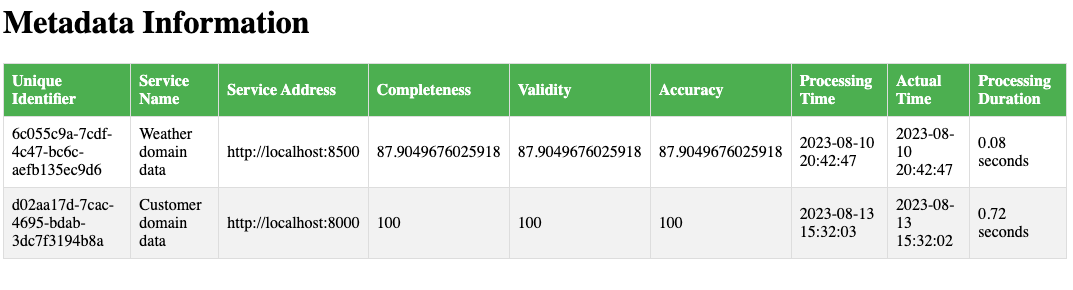
\includegraphics[width=\textwidth]{images/Datalichen-dashboard.png}

  \caption{Data Lichen Dashboard in Local Development Environment} 

  \label{dataLichenDashboard}

\end{figure*}

\begin{figure*}[ht]

  \centering

  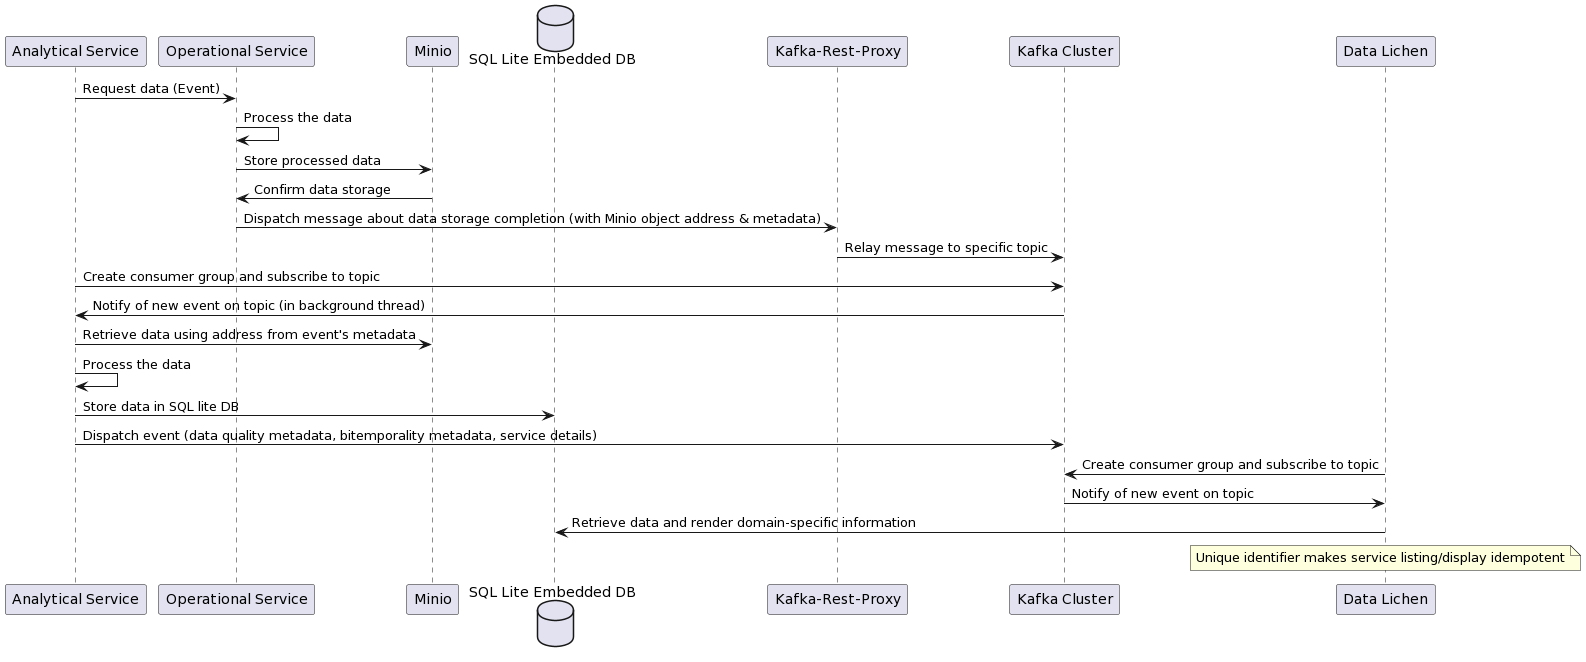
\includegraphics[width=\textwidth]{images/intra-domain-flow.jpg}

  \caption{Intra-domain communication in Terramycelium's prototype}

  \label{intraDomain}

\end{figure*}

Domain A requests a 5GB JSON file from domain B in this instance. Domain A possesses the meteorological data, but Domain B possesses the customer ratings and business data. An event is sent from the domain A to Data Lichen to obtain a list of all datasets along with metadata such as actual time, processing time, completeness, and correctness. 

The information contains the address of the data domain to be retrieved. The address is utilised to send an event to domain B for data retrieval. This activates the internal process of domain B, leading to the production and storage of datasets in the distributed storage service. After the procedure is finished, an event is sent to the data processing completion topic, to which domain A is subscribed. Figure~\ref{kafkaTopics} provides an overview of the Kafka topics utilised in this investigation.

\begin{figure*}[ht]

  \centering

  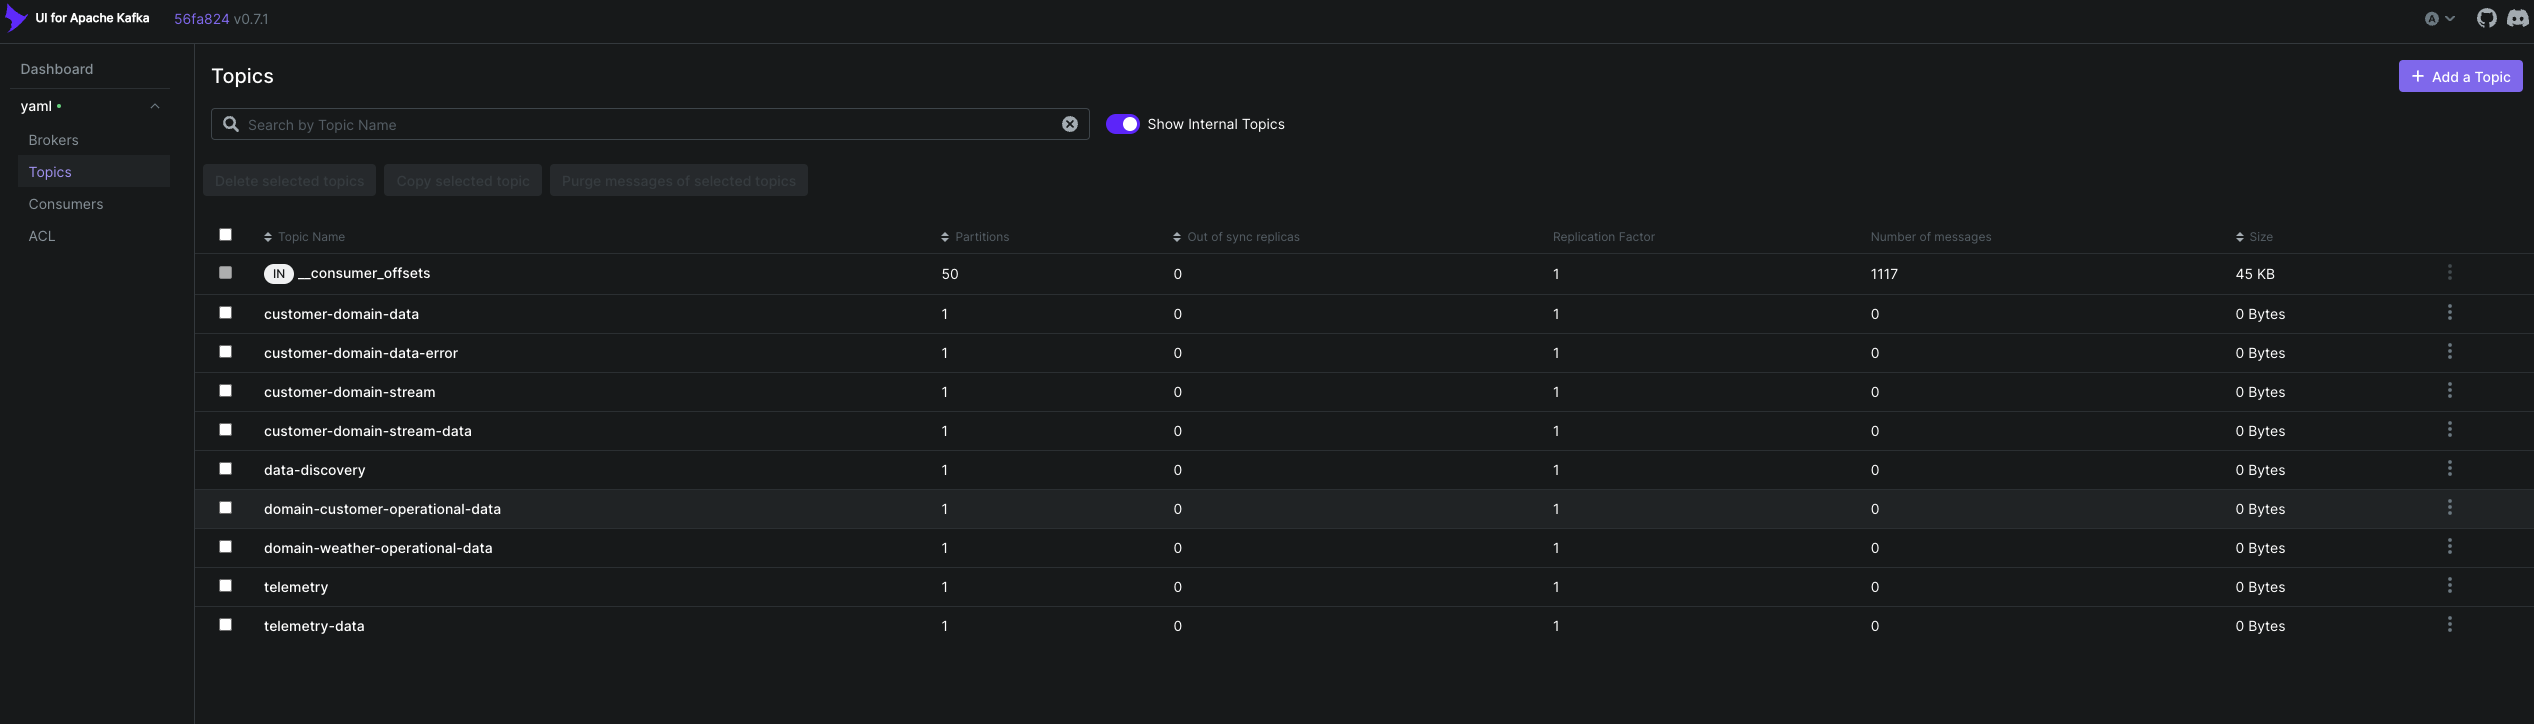
\includegraphics[width=\textwidth]{images/kafka-topics.png}

  \caption{Overview of kafka topics}

  \label{kafkaTopics}

\end{figure*}

The event signalling the conclusion of data processing also includes the data address. Domain A utilises this URL to retrieve the data. After retrieving the data, it is subsequently processed. The flow is illustrated in Figure~\ref{s1Flow}.

\begin{figure*}[ht]

  \centering

  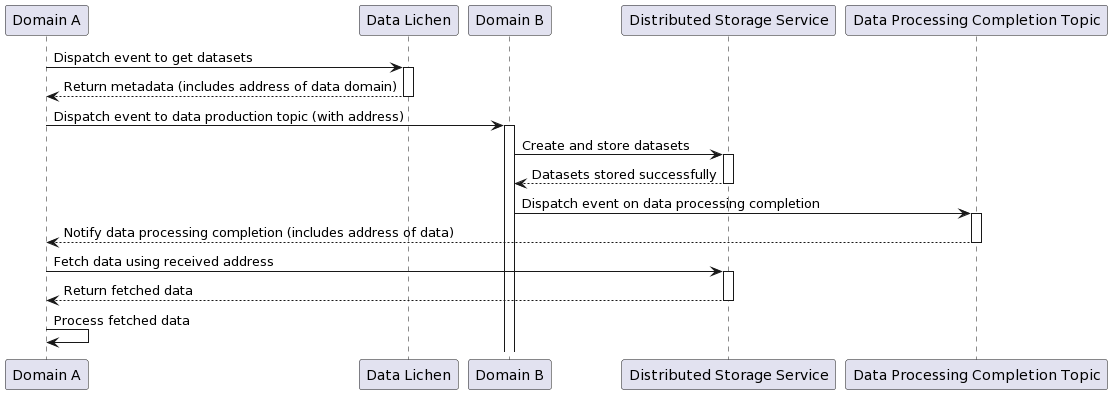
\includegraphics[width=\textwidth]{images/Scenario-s1.png}

  \caption{Scenario S-1 Flow Diagram}

  \label{s1Flow}

\end{figure*}

Understanding system performance and resource utilisation is crucial in this scenario. Data ingestion rate is a direct indicator of the system's throughput, showing how effectively the system can handle large volumes of incoming data. A high rate indicates efficient data processing capability, which is crucial for situations with an anticipated fast data influx. Latency, divided into intake and processing components, provides an understanding of system responsiveness. Minimal latency is essential for ensuring prompt data availability and processing, especially in systems where delays can cause subsequent effects. 

CPU usage and memory utilisation are key metrics for assessing the system's resource efficiency. Increased CPU or memory usage could signal bottlenecks, inefficiencies, or places that could be optimised, particularly during times of high demand. The error rate provides information on the system's resilience and dependability. A low error rate, even with large amounts of data, indicates the system's ability to continuously manage and process data without any issues. 

These metrics collectively evaluate the system's capacity to sustain performance and stability when faced with high data input requirements. Each measure will be described in connection to the corresponding system mechanism in the following sections.

\paragraph{Data Ingestion Rate}

Each service is instrumented using OpenTelemetry SDKs to capture telemetry data for FastAPI requests and manual spans for specified processes. The collected data is then exported to Kafka using the KafkaRESTProxyExporter class to measure the data intake rate. 

Figure~\ref{openTelemetryTopic} illustrates the open telemetry Kafka topic and a large number of events recorded in this topic. The open telemetry processor service consumes all events sent to this topic. The service gathers and maintains metrics, which are then extracted by Prometheus and subsequently sent to Grafana. The flow is depicted in Figure~\ref{openTelemetryFlow}. The JSON displayed in Figure~\ref{openTelemetryTraceSpan} depicts an example of a trace span JSON that is communicated over Kafka to the open telemetry service.

\begin{figure*}[ht]

  \centering

  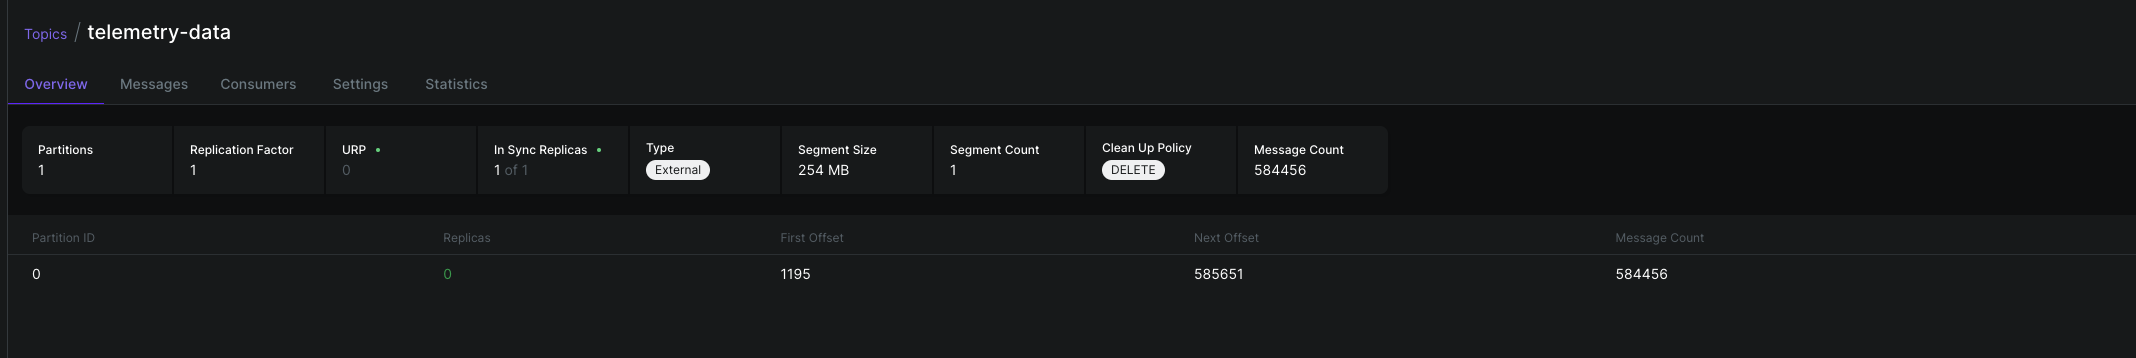
\includegraphics[width=\textwidth]{images/kafka-open-telemetry-topic-screenshot.png}

  \caption{Open Telemetry Topic}

  \label{openTelemetryTopic}

\end{figure*}

\begin{figure*}[ht]

  \centering

  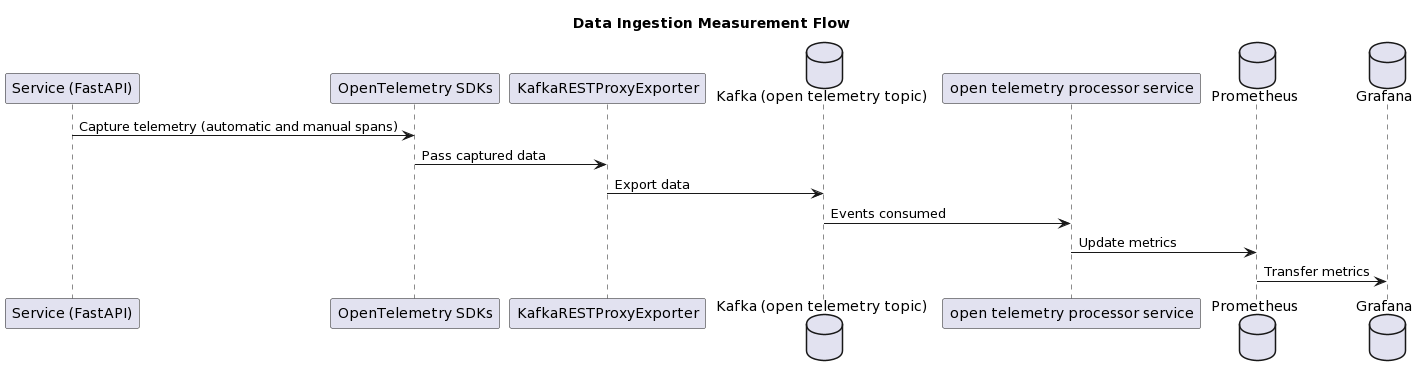
\includegraphics[width=\textwidth]{images/open-telemetry-flow.png}

  \caption{Open Telemetry Flow}

  \label{openTelemetryFlow}

\end{figure*}

\begin{figure}[!ht]

  \centering

  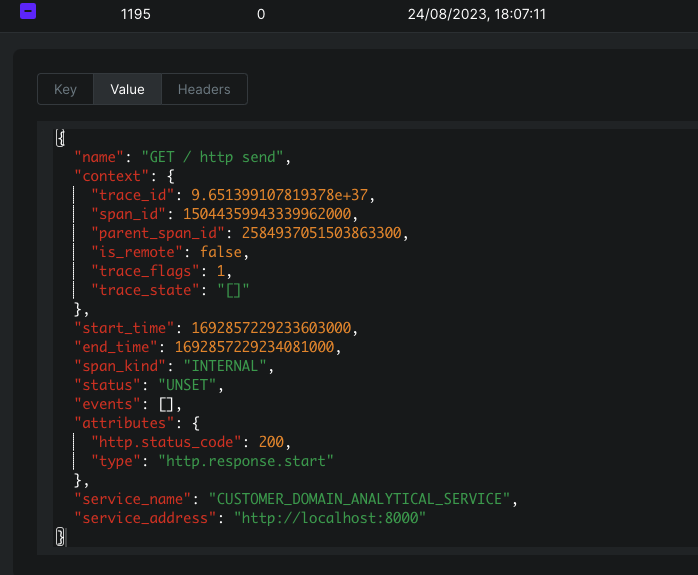
\includegraphics[width=\columnwidth]{images/open-telemetry-trace-example.png}

  \caption{Open Telemetry Trace Span}

  \label{openTelemetryTraceSpan}

\end{figure}

Before presenting the experiment results, it is important to define the specific meaning of heavy load of data' in the context of this study. In BD, there is no commonly accepted criterion for defining high volume', particularly in decentralised, domain-driven architectures such as Terramycelium. There is no single standard benchmark that universally defines what qualifies as a heavy data load in these systems. 

Academic research and business reports suggest that daily data intake can reach terabytes or more, particularly in high-velocity streams such as social media or e-commerce transactions \cite{AtaeiBigDataEnvirons}. 

Transferring many gigabytes of data in JSON format between domains is a substantial stress test due to its verbosity and demands compared to binary formats. The Yelp academic dataset is divided into 400KB chunks and transferred many times to test the prototype's capability and resilience against increased data traffic. 

This configuration is suitable for practical scenarios where systems need to consistently handle continuous streams of incoming data from different sources and varying quantities, while maintaining high performance and data integrity. Terramycelium's decentralised, event-driven architecture is designed to allow data to be smoothly ingested, processed, and retrieved, regardless of the frequency of dataset transfers or accesses. This assesses the system's capacity to manage large amounts of data and its ability to perform well in a setting that replicates the rapid data flow typical of modern BD scenarios.

All data sent during the experiment is stored in MinIO. Upon successful storage, a confirmation is always sent back. The process of streaming, storing, and validating data was repeated several times to demonstrate its reliability, especially when dealing with large amounts of data. Reliable and accurate communication in challenging situations supports the importance of consistent communication in remote systems, as shown in the works of Kleppmann \cite{Kleppmann2017}. The process can be formally represented using logical implications to determine the system's resilience.

Let's denote the following:

\begin{itemize}

    \item \( P \) as the event where ``data is transferred from Domain A to Domain B''.

    \item \( Q \) as the event where ``data is successfully stored in MinIO''.

    \item \( R \) as the event where ``confirmation of successful storage is communicated back''.

\end{itemize}

From the empirical observations, it is deduced that:

\[ P \quad \text{implies} \quad Q \]

\[ Q \quad \text{implies} \quad R \]

Thus, utilising the transitive property of implications \cite{johnson2019logic}, it is inferred that:

\[ P  \quad \text{implies} \quad R \]

Every data transmission from Domain A to Domain B ensures the certification of successful storage. The link highlights the system's effectiveness and dependability in handling extensive amounts of data, aligning with the conclusions of Lee \cite{lee2020bigdata} who stressed the need to maintain data consistency and integrity in distributed storage systems. 

The graph in Figure~\ref{kafkIngestionInBytesInCustomerDomainAnalyticalService} shows that the Kafka data ingestion reached its highest point at 1,693,816,791 bytes on 2023-09-04 at 20:40:00 in the analytical service of the customer domain, demonstrating the transfer of data from the operational service to the analytical service. The bar chart illustrates the incremental rise in the service's workload.  The entire quantity of data ingested during the trial was 1.6 billion bytes, as shown in Figure~\ref{totalDataIngestedinBytesInCustomerDomainsAnalyticalService}.

\begin{figure*}[ht]

  \centering

  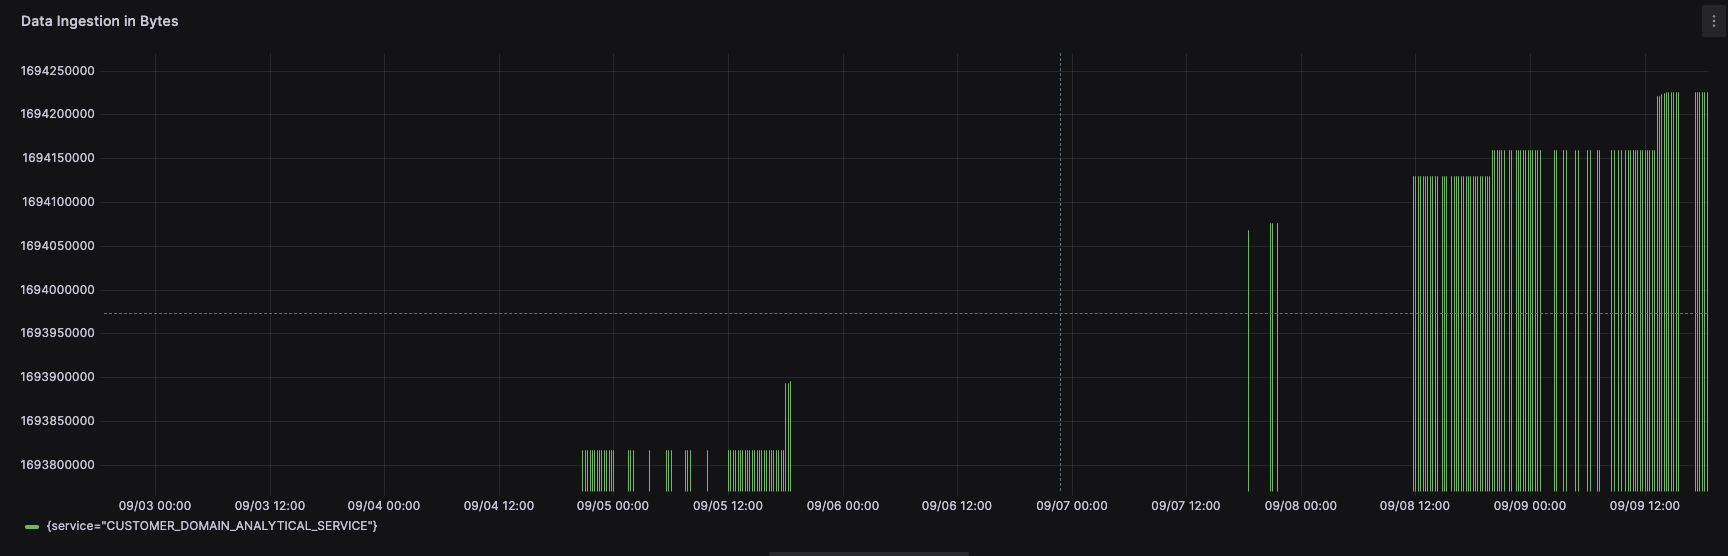
\includegraphics[width=\linewidth]{images/Kafka-ingestion-in-Bytes.png}

  \caption{Kafka Data Ingestion in Bytes in Customer Domain's Analytical Service}

  \label{kafkIngestionInBytesInCustomerDomainAnalyticalService}

  \end{figure*}

\begin{figure}[ht]

  \centering

  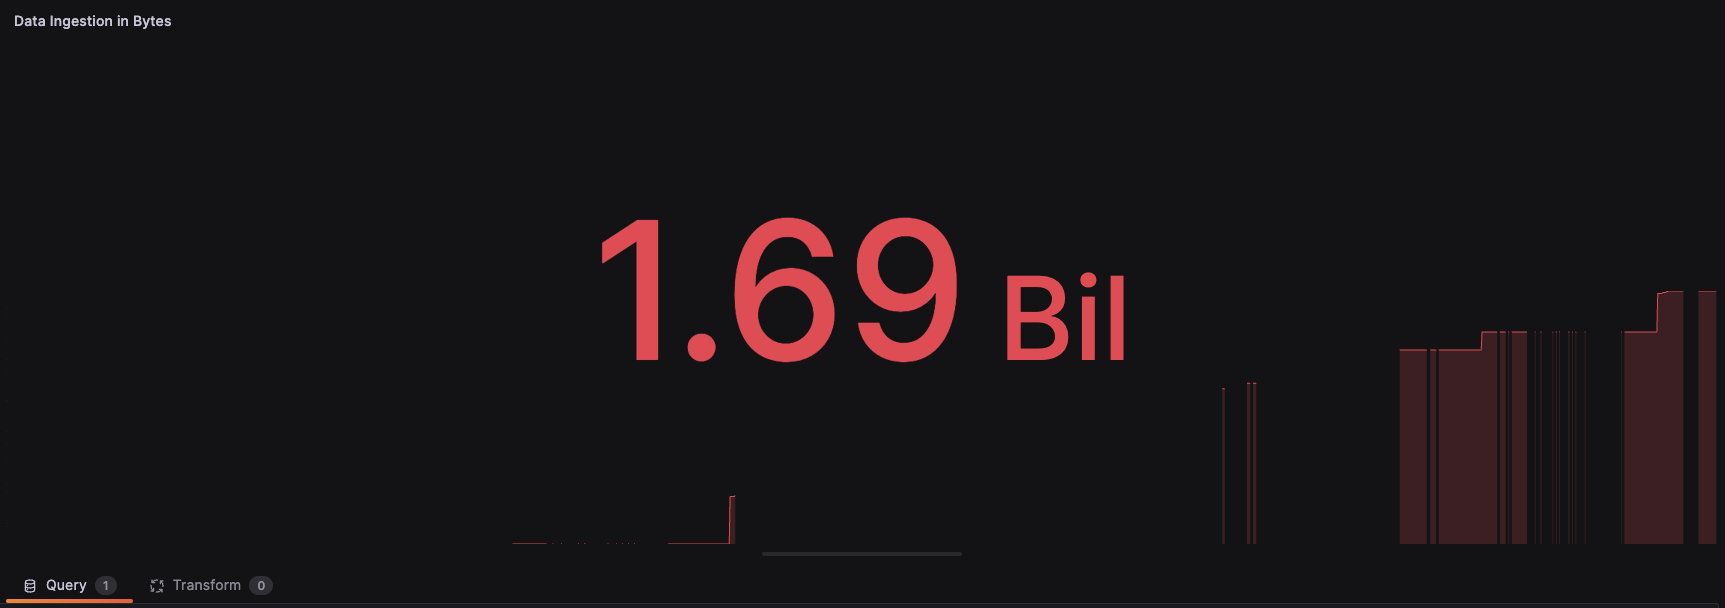
\includegraphics[width=\columnwidth]{images/total-data-ingested-in-bytes.jpeg}

  \caption{Total Data Ingested in Bytes in Customer Domains' Analytical Service}

  \label{totalDataIngestedinBytesInCustomerDomainsAnalyticalService}

\end{figure}

The data ingestion rate for the weather domain's analytical service peaked at 1,693,893,416 bytes on September 5, 2023, at 18:00:00, as shown in Figure~\ref{totalDataIngestedinBytesInWeatherDomainsAnalyticalService}. This service has processed a total of 1.6 billion bytes.

\begin{figure*}[ht]

  \centering

  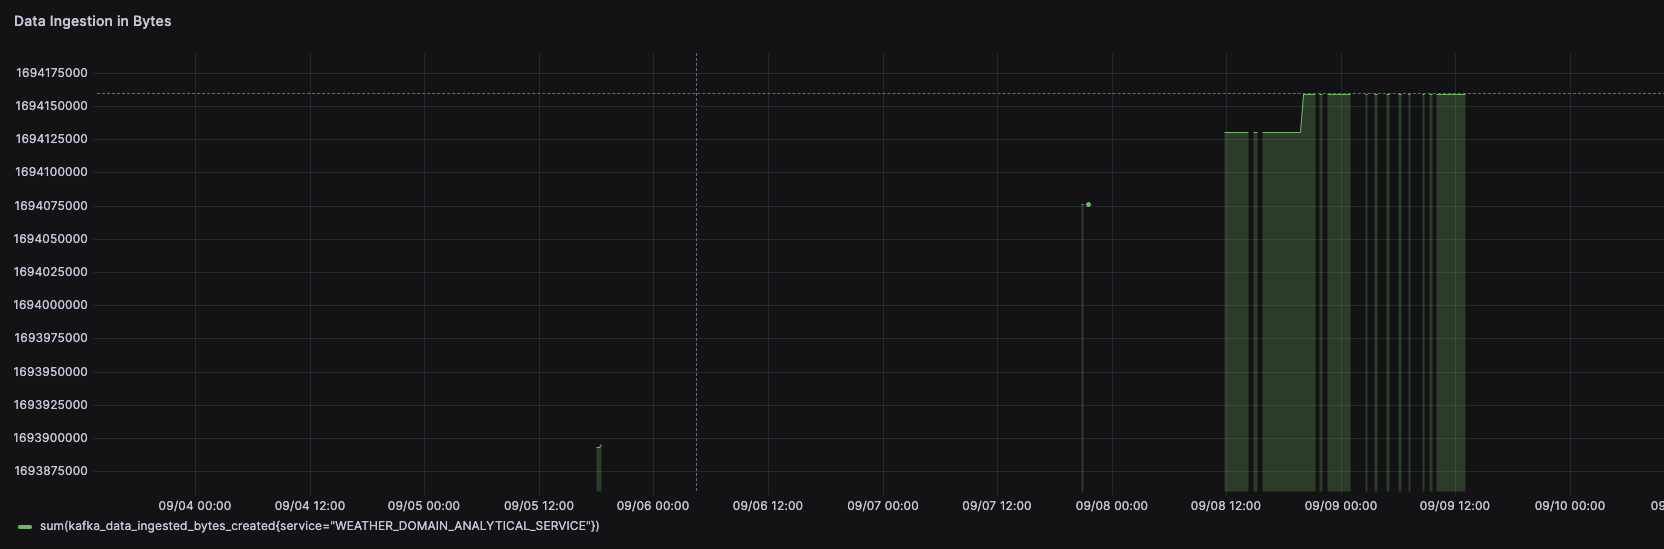
\includegraphics[width=\textwidth]{images/weather-domain-ingested-data-in-bytes.png}

  \caption{Total Data Ingested in Bytes in Weather Domain's Analytical Service}

  \label{totalDataIngestedinBytesInWeatherDomainsAnalyticalService}

\end{figure*}

The system's performance during large data input is empirically evaluated by visualising metrics in Grafana using the screenshots. The monitoring system offers timestamped data points showing the amount of data consumed at different intervals. The Table~\ref{dataIngestedInCustomerDomainAnalyticalServiceTable} records the data points collected within a particular time frame in the analytical service of the customer domain.

\begin{table}[ht]

  \centering

  \caption{Data Ingested in Customer Domain's Analytical Service}

  \begin{tabular}{|c|c|}

  \hline

  \textbf{Timestamp} & \textbf{Data Ingested (bytes)} \\

  \hline

  2023-09-04 20:40:00 & 1693816791 \\

  2023-09-04 20:45:00 & 1693816791 \\

  2023-09-04 20:50:00 & 1693816791 \\

  2023-09-04 20:55:00 & 1693816791 \\

  2023-09-04 21:00:00 & 1693816791 \\

  2023-09-04 21:05:00 & 1693816791 \\

  2023-09-04 21:10:00 & 1693816791 \\

  2023-09-04 21:15:00 & 1693816791 \\

  2023-09-04 21:20:00 & 1693816791 \\

  2023-09-04 21:25:00 & 1693816791 \\

  2023-09-04 21:30:00 & 1693816791 \\

  2023-09-04 21:35:00 & 1693816791 \\

  \hline

  \end{tabular}

  \label{dataIngestedInCustomerDomainAnalyticalServiceTable}

\end{table}

In addition, the data acquired in the analytical service of the weather domain is presented in the Table \ref{dataIngestedInWeatherDomainAnalyticalServiceTable}. After capturing the ingestion rate in bytes, it is essential to further explore other metrics to provide a comprehensive analysis of the system's performance during high data load conditions.

\begin{table}[ht]

  \centering

  \caption{Data Ingested in Weather Domain's Analytical Service}

  \begin{tabular}{|c|c|}

  \hline

  \textbf{Timestamp} & \textbf{Data Ingested (bytes)} \\

  \hline

  2023-09-05 18:00:00 & 1693893416 \\

  2023-09-05 18:15:00 & 1693893416 \\

  2023-09-05 18:30:00 & 1693895179 \\

  2023-09-07 20:45:00 & 1694076236 \\

  2023-09-07 21:00:00 & 1694076236 \\

  2023-09-07 21:30:00 & 1694076236 \\

  2023-09-08 11:45:00 & 1694130131 \\

  2023-09-08 12:00:00 & 1694130131 \\

  2023-09-08 12:15:00 & 1694130131 \\

  2023-09-08 12:30:00 & 1694130131 \\

  2023-09-08 12:45:00 & 1694130131 \\

  2023-09-08 13:00:00 & 1694130131 \\

  \hline

  \end{tabular}

  \label{dataIngestedInWeatherDomainAnalyticalServiceTable}

\end{table}

\paragraph{Ingestion Latency}

Ingestion latency measures the time between when a data record is published to Kafka and when it is processed by the domains. It is calculated for each Kafka record that is ingested using a specific formula.

\[ Latency = current\_time - publish\_time \] 

Where:

\begin{itemize}

    \item \(current\_time\) denotes the time at which the record is being processed.

    \item \(publish\_time\) represents the timestamp when the record was published to Kafka. If the Kafka record lacks a timestamp, the current time is assigned as a default, making the latency calculation a fallback measure.

\end{itemize}

The latency numbers captured are presented in Figure~\ref{cusetomerAndWeatherDomainAnalyaticalServicesLatencies}. The figure shows that the latency in both domains' analytical services is negligible, with one spike reaching 400 seconds and the rest maintaining a constant ingestion latency of roughly 50 to 100 seconds. The weather domain experiences lower latency than customer latency, averaging 50 seconds. This is because this domain uses a less amount of data.

\begin{figure*}[ht]

  \centering

  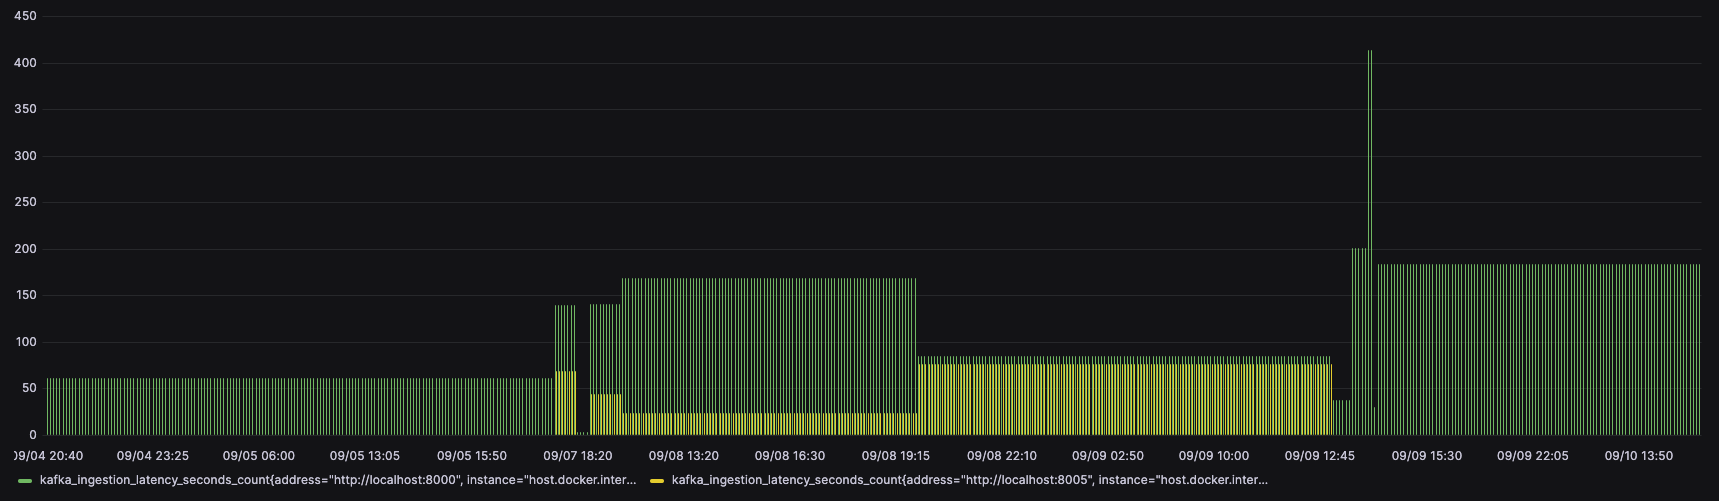
\includegraphics[width=\textwidth]{images/customer-and-weather-domain-analytics-service-latency.png}

  \caption{Customer and Weather Domain's Analytical Service Latencies}

  \label{cusetomerAndWeatherDomainAnalyaticalServicesLatencies}

\end{figure*}

The findings are significant given the intricacies and asynchronous nature of the domain-driven distributed BD system utilising Kafka. The occasional increase to 400 seconds in ingestion latency is noteworthy but falls within acceptable limits, particularly given Kafka's internal features like indexing methods, offset management, and sticky partition behaviour.

\paragraph{CPU Usage} \label{cpuUsageInS1}   

The telemetry processing service is crucial to the infrastructure and offers valuable information when monitoring CPU utilisation. It is crucial to monitor this service since it provides immediate insights into data processing efficiency. Therefore, increased CPU utilisation in this service implies potential processing bottlenecks. 

Furthermore, CPU utilisation metrics are calculated at certain intervals. Due to the asynchronous nature of receiving telemetry data from different services, monitoring the CPU consumption of individual services may not provide an accurate representation of the current system load. The telemetry service consistently processes data to ensure that its measurements accurately reflect the system's load. 

It is important to consider this finding while assessing scalability and forecasting future infrastructure needs. CPU consumption measurements can be affected by the operating system and environment in which the services are running. The given statistics may not be exact, but they provide a reliable comparison of system resource usage.

Figure~\ref{openTelemetryServiceCpuUsage} illustrates the CPU utilisation trends of the telemetry processing service, emphasising the interplay between data intake rates and resource consumption.

\begin{figure*}[ht]

    \centering

    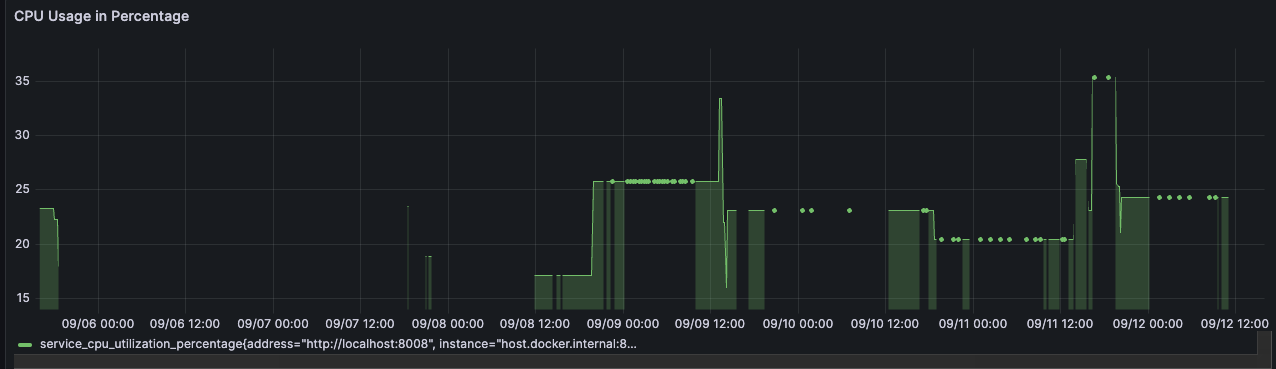
\includegraphics[width=\textwidth]{images/Open-telemetry-service-CPU-usage.png}

    \caption{Open Telemetry Service CPU Usage}

    \label{openTelemetryServiceCpuUsage}

\end{figure*}

The CPU utilisation in the Open Telemetry service metrics shows a continuous level of around 24 percent, with occasional peaks reaching 25.8 percent at certain times. The behaviour is a result of the architecture in which events are consistently transmitted to the associated services. A full table showing the CPU utilisation during a certain period can be found in Table~\ref{table:telemetry-cpu-usage} to clarify this issue. The tabulation offers insights into the variation in CPU usage at different times and under varied conditions, showing periods of stable CPU usage, periods of inactivity, and occasional spikes in utilisation.

\begin{table}[!ht]

  \centering

  \begin{tabular}{|l|l|}

  \hline

  \textbf{Date and Time} & \textbf{Average CPU Usage (\%)}        \\ \hline

  09/06 00:00           & 23\%, 24\%                             \\ \hline

  09/06 12:00           & 0 (no processes)                       \\ \hline

  09/07 00:00           & 0 (no processes)                       \\ \hline

  09/07 12:00           & 0 (no processes)                       \\ \hline

  09/08 00:00           & 24\%, 18\%                             \\ \hline

  09/08 12:00           & 17\%                                   \\ \hline

  09/09 00:00           & 26\%                                   \\ \hline

  09/09 12:00           & 26\% (with a spike to 34\%)            \\ \hline

  09/10 00:00           & 24\%                                   \\ \hline

  09/10 12:00           & 24\%                                   \\ \hline

  09/11 00:00           & 22\%                                   \\ \hline

  09/11 12:00           & 22\% (with spikes to 27\% and 35.2\%)  \\ \hline

  09/12 00:00           & 24\%                                   \\ \hline

  09/12 12:00           & 24\%                                   \\ \hline

  \end{tabular}

  \caption{Telemetry Processing Service CPU Utilisation}

  \label{table:telemetry-cpu-usage}

\end{table}

The constant and regular CPU usage indicates a reliable processing environment. Stability can indicate optimised data streaming, where the telemetry service efficiently manages incoming events without excessive resource usage or sudden computational spikes. 

The Kubernetes cluster CPU use consistently stays at 43\%, with occasional spikes up to 250\% as seen in Figure~\ref{kubernetesClusterCpuUsage}. These spikes typically occur when a large amount of data is being sent across the network and into Minio.

\begin{figure}[ht]

  \centering

  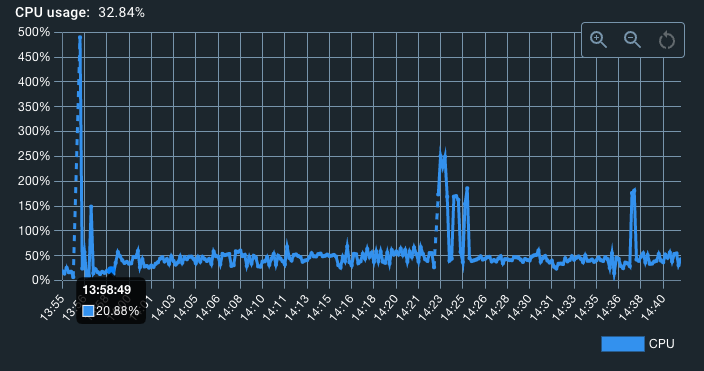
\includegraphics[width=\columnwidth]{images/kubernetes-cluster-CPU-usage.png}

  \caption{Kubernetes Cluster CPU Usage}

  \label{kubernetesClusterCpuUsage}

\end{figure}

Similarly, as shown in Figure~\ref{kubernetesClusterReadAndWrite}, an average of 5.37GB of data was read and 12.2GB of data was written at various intervals. Furthermore, the network has received 11.6 gigabytes of data and delivered 13.9 megabytes (Figure~\ref{kubernetesClusterNetworkStatistics}).

\begin{figure}

  \centering

  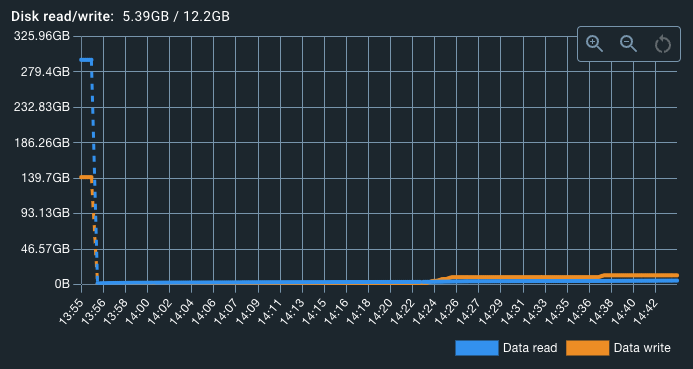
\includegraphics[width=\columnwidth]{images/Kubernetes-cluster-data-read-write.png}

  \caption{Kubernetes Cluster Read and Write Statistics}

  \label{kubernetesClusterReadAndWrite}

\end{figure}

\begin{figure}

  \centering

  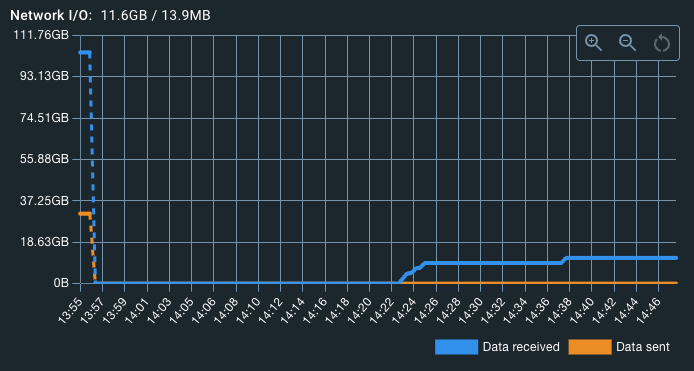
\includegraphics[width=\columnwidth]{images/kubernetes-cluster-network-data-received-and-sent.png}

  \caption{Kubernetes Cluster Network Statistics}

  \label{kubernetesClusterNetworkStatistics}

\end{figure}

After thoroughly analysing the telemetry and infrastructure data, it is clear that the asynchronous and event-driven architecture of this BD architecture positively impacts its performance dynamics. In this asynchronous event-driven paradigm, it is important to acknowledge that the amount of data handled, measured in gigabytes, is less important than the system's efficiency in handling incoming data streams.

The telemetry service demonstrates its resilience in data processing by maintaining a continuously moderate CPU consumption, even when faced with fluctuating data input rates. Similarly, the Kubernetes cluster occasionally experiences surges in CPU utilisation during data-intensive tasks, but overall it maintains a well-distributed workload. This is evidence of the system's proficiency in handling and allocating work among its nodes.

The data statistics about read, write, and network transfers provide additional clarification on this matter. Although the amount of data being read, written, or transported in gigabytes may appear substantial, what truly matters is not the sheer number but rather the system's efficiency in managing these processes. The average data read is 5.37 GB, and the average data written is 12.2GB. These figures, when compared to the network statistics shown in Figure~\ref{kubernetesClusterNetworkStatistics}, demonstrate the system's effectiveness in managing data and performing network operations without becoming overloaded.

The metrics not only demonstrate the stability and efficiency of the BD infrastructure but also offer empirical evidence that, in an event-driven asynchronous system like Terramycelium, the focus is not solely on the amount of data processed but rather on the effectiveness and reliability with which it is managed. This observation indicates possible consequences for scalability considerations in future implementations of similar architectures.

\paragraph{Memory Utilisation}

Memory utilisation is a crucial measure when assessing system efficiency. An efficient memory management system demonstrates a system's capability to process real-time data and adapt to varying workloads. The memory usage seen in the telemetry processing service, a vital element of the infrastructure, offers precise insights into the system's ability to handle data. Examining these memory patterns provides a more distinct comprehension of the service's effectiveness in handling different data rates and identifies places where memory optimisation may be required to improve overall performance.

In the weather domain, memory utilisation can be categorised into two primary types: operational services and analytical services. Operational services that serve static data have low memory usage because they require less processing power. On the other hand, analytical services can exhibit diverse memory patterns based on the intricacy of data analysis.

The customer domain has the same pattern, wherein operational services have consistent memory use as a result of predominantly handling static client data. On the other side, the analytical services, which thoroughly examine client habits and preferences, may experience occasional surges, particularly when dealing with large datasets.

The memory utilisation trends across the various services are visualised in Figure~\ref{kubernetesClusterMemoryUsage}. The address for each service is specified in the respective service definitions in the Github repositories \cite{terramyceliumInfrastructure,terramyceliumHelmChartsAndApplications}. It is important to note that the service running on port 8000 is the operational service in the customer domain, while the service on port 8001 is the analytical service for the customer domain. The service running on port 8005 is the operational service for the weather domain, whereas the service on port 8006 is the analytical service for the same domain. The service running on port 8008 is the application responsible for processing telemetry data.

\begin{figure}

  \centering

  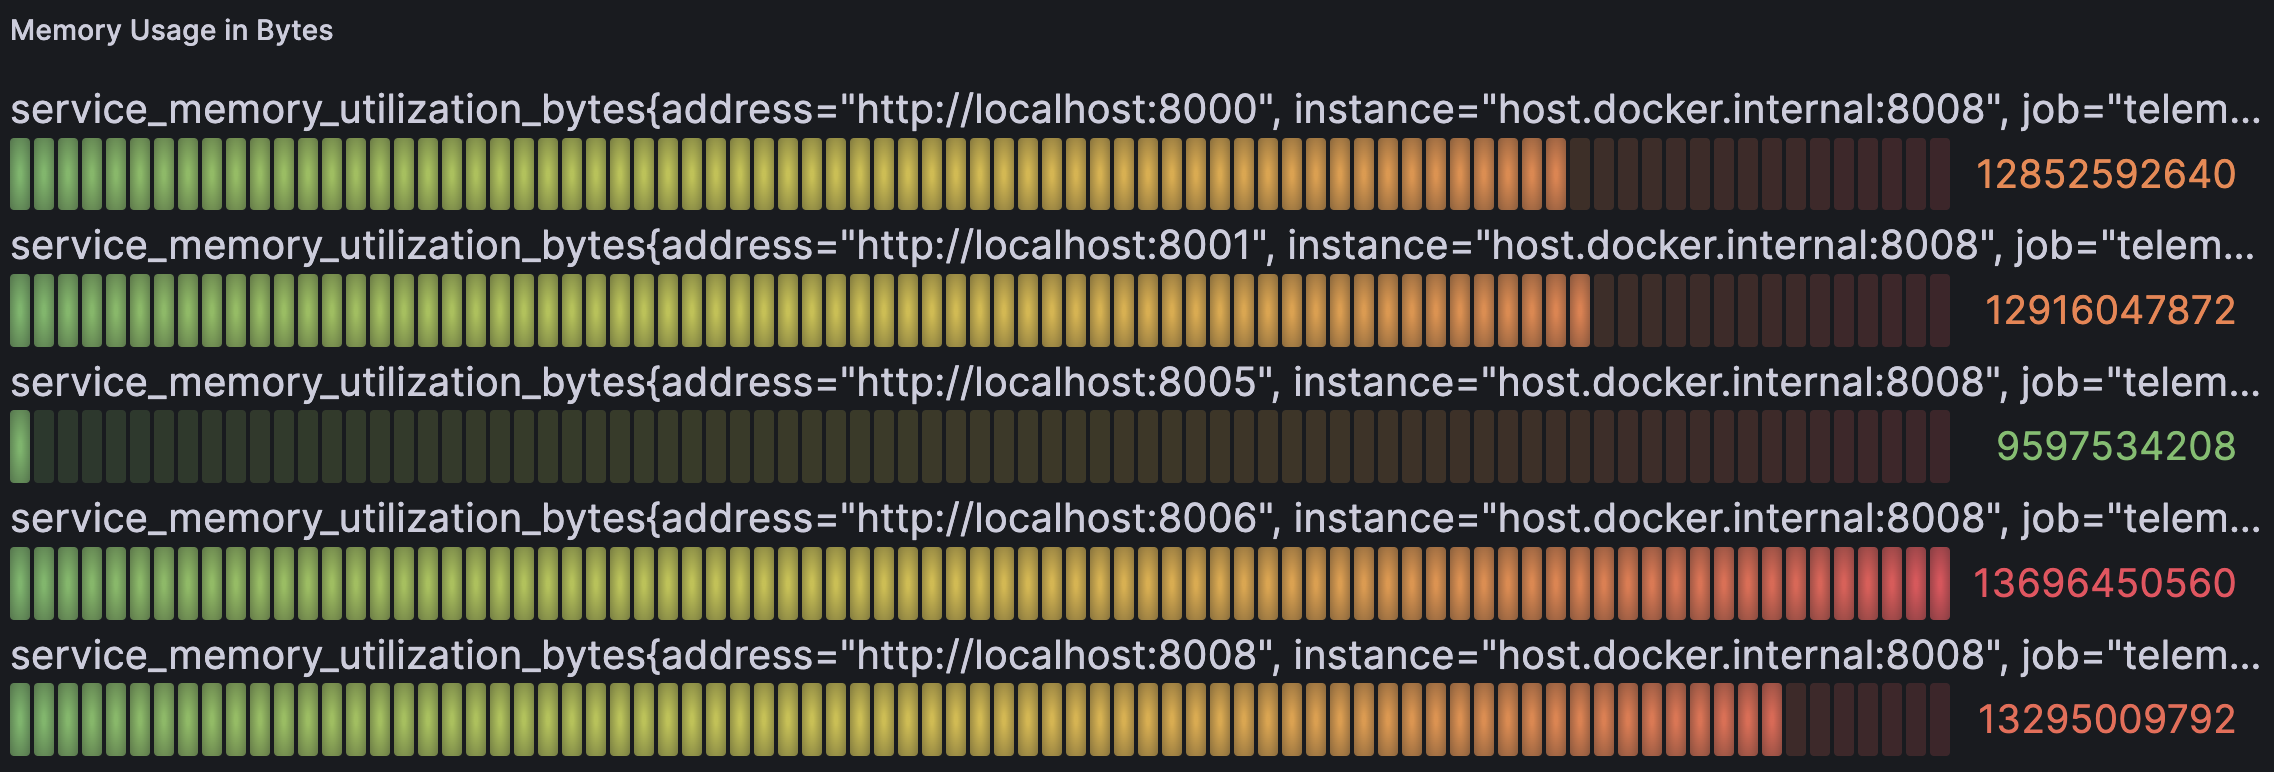
\includegraphics[width=\columnwidth]{images/Memory-usage-for-various-services-in-kube.png}

  \caption{Memory Usage for Various Services in the Cluster}

  \label{kubernetesClusterMemoryUsage}

\end{figure}

The association between CPU and memory usage is further explained in Table~\ref{table:memory-cpu-correlation}. This table illustrates the allocation of memory across several services at specific instances of CPU use. It is evident that periods of increased CPU activity align with higher memory allocation, especially in the telemetry processing service. This alignment clarifies the system's ability to scale and respond effectively during moments of high computing demand. 

Similarly, as the CPU utilisation decreases, there is also a decrease in the amount of memory being used, which highlights the effective management of resources during periods of less demanding processing. The ability to efficiently use memory in a way that can adapt to different needs is crucial for sustaining the performance of a system and ensuring that real-time data is managed smoothly across the entire infrastructure.

\begin{table}[htbp]
    \centering
    \resizebox{\textwidth}{!}{%
      \begin{tabular}{|l|l|l|l|l|l|}
        \hline
        \textbf{Date \& Time} & \textbf{Svc A (B)} & \textbf{Svc B (B)} & \textbf{Svc C (B)} & \textbf{Svc D (B)} & \textbf{Svc E (B)} \\
        \hline
        09/06 00:00 & H (12,750,000,000) & H (12,800,000,000) & L (4,700,000,000) & H (14,000,000,000) & H (13,500,000,000) \\
        \hline
        09/06 12:00 & L (6,350,000,000) & L (6,400,000,000) & L (4,650,000,000) & M (10,850,000,000) & M (10,650,000,000) \\
        \hline
        09/07 00:00 & L (6,375,000,000) & L (6,425,000,000) & L (4,675,000,000) & M (10,870,000,000) & M (10,670,000,000) \\
        \hline
        09/07 12:00 & L (6,360,000,000) & L (6,410,000,000) & L (4,680,000,000) & M (10,860,000,000) & M (10,660,000,000) \\
        \hline
        09/08 00:00 & M (9,560,000,000) & M (9,610,000,000) & L (4,720,000,000) & H (13,800,000,000) & H (13,300,000,000) \\
        \hline
        09/08 12:00 & M (9,580,000,000) & M (9,630,000,000) & L (4,750,000,000) & H (13,850,000,000) & H (13,350,000,000) \\
        \hline
        09/09 00:00 & H (12,780,000,000) & H (12,830,000,000) & L (4,770,000,000) & H (14,100,000,000) & H (13,600,000,000) \\
        \hline
        09/09 12:00 & H (12,760,000,000) & H (12,810,000,000) & L (4,760,000,000) & H (14,050,000,000) & H (13,550,000,000) \\
        \hline
        09/10 00:00 & M (9,570,000,000) & M (9,620,000,000) & L (4,730,000,000) & M (10,900,000,000) & M (10,700,000,000) \\
        \hline
        09/10 12:00 & M (9,590,000,000) & M (9,640,000,000) & L (4,740,000,000) & M (10,920,000,000) & M (10,680,000,000) \\
        \hline
        09/11 00:00 & M (9,565,000,000) & M (9,615,000,000) & L (4,710,000,000) & M (10,880,000,000) & M (10,670,000,000) \\
        \hline
        09/11 12:00 & H (12,770,000,000) & H (12,820,000,000) & L (4,775,000,000) & H (14,110,000,000) & H (13,610,000,000) \\
        \hline
        09/12 00:00 & M (9,585,000,000) & M (9,635,000,000) & L (4,745,000,000) & M (10,930,000,000) & M (10,690,000,000) \\
        \hline
        09/12 12:00 & M (9,600,000,000) & M (9,650,000,000) & L (4,755,000,000) & M (10,950,000,000) & M (10,700,000,000) \\
        \hline
      \end{tabular}%
    }
    \caption{Correlated Memory and CPU Usage for Various Services. Legend: B - Bytes, H - High Usage, M - Medium Usage, L - Low Usage. Service A corresponds to localhost:8000, B to localhost:8001, C to localhost:8005, D to localhost:8006, and E to localhost:8008.}
    \label{table:memory-cpu-correlation}
\end{table}



\paragraph{Error Rate}

Error rates within the FAST API services are determined through analysis of logs and monitoring of exception blocks. Every domain is assigned a specific Kafka topic exclusively for the purpose of reporting errors. However, as depicted in Figure~\ref{numberOfErrorsInTelemetryProcessingService}, only the OpenTelemetry service encountered issues. However, the weather and customer domains did not have any errors.

The intrinsic ability of event-driven systems to recover quickly and effectively adds greatly to the low occurrence of errors. The decoupling between components in these systems guarantees that transitory errors in one service are typically contained, preventing them from spreading and causing interruptions throughout the entire system. This tendency is clearly seen in the prototype, highlighting the inherent advantages of event-driven architectures in ensuring the resilience of the system. The term "peak" refers to the highest point or maximum value of something. It represents the culmination, or apex, of a certain phenomenon or trend.

\begin{figure}

  \centering

  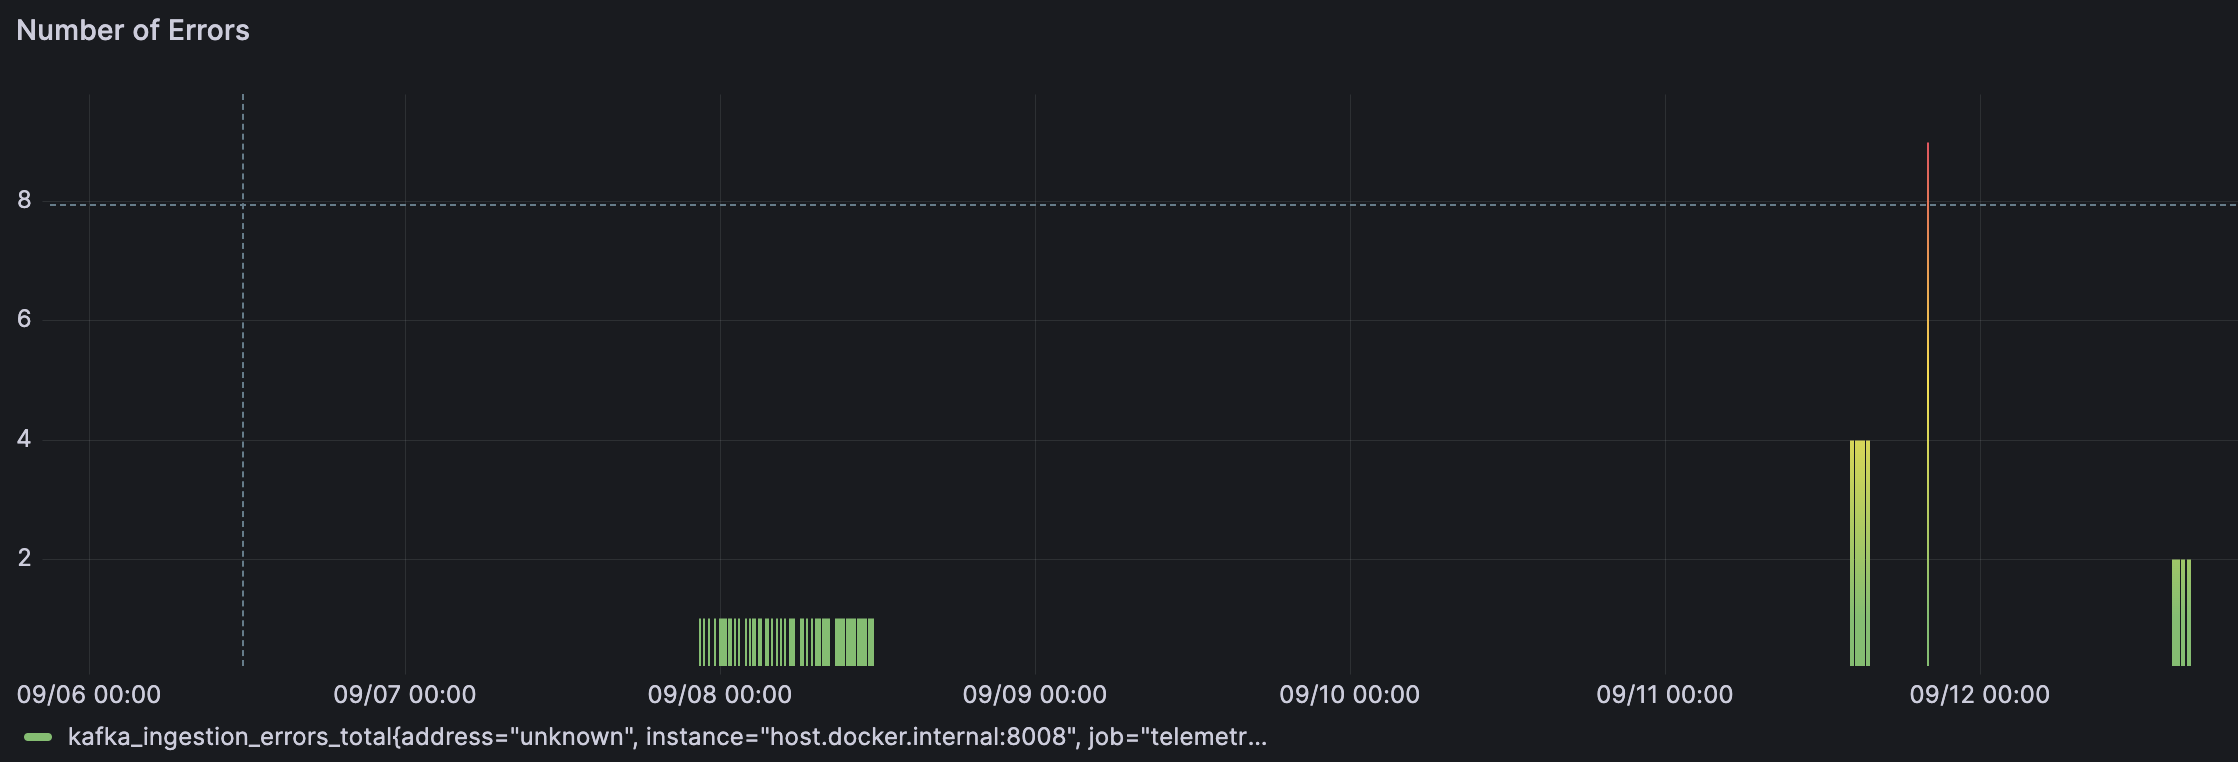
\includegraphics[width=\columnwidth]{images/number-of-errors-in-telemetry-processing-service.png}

  \caption{Number of Errors in Telemetry Processing Service}

  \label{numberOfErrorsInTelemetryProcessingService}

\end{figure}

With the above metrics in conjunction with the ingestion rate, a comprehensive understanding of the system's operational efficiency, resilience, and overall performance can be obtained.

\subsubsection{Scenario S2: High Velocity Data Ingestion Scenario}

Scenario S2 tests the system's capabilities under high data velocity conditions, approximating peak ingestion rates. This experiment involved Domain A (Customer Domain) streaming data into Domain B (Weather Domain), with Domain B subsequently processing the streamed data. To facilitate this, a dedicated Kafka topic, named customer-domain-stream-data, is established, earmarking it exclusively for the streaming operations between the two domains. 

Concurrently, within the customer domain, a novel endpoint is created. This endpoint is responsible for streaming out the data that had been previously stored. In synchrony with this, the weather domain analytical service adopts a long-polling mechanism. By doing so, it could efficiently subscribe to and intake the continuous data stream relayed from the customer domain.

A methodical analysis is conducted based on the metrics of interest:

\paragraph{Volume and Size of Messages} The system processed a total of 771,305 messages. Collectively, these messages have a combined volume of around 1 GB, and they are all sent to the customer-domain-stream-data topic. The statistical data related to the streaming subject is illustrated in Figure~\ref{customerDomainStreamingTopicStatistics}.

\begin{figure}

  \centering

  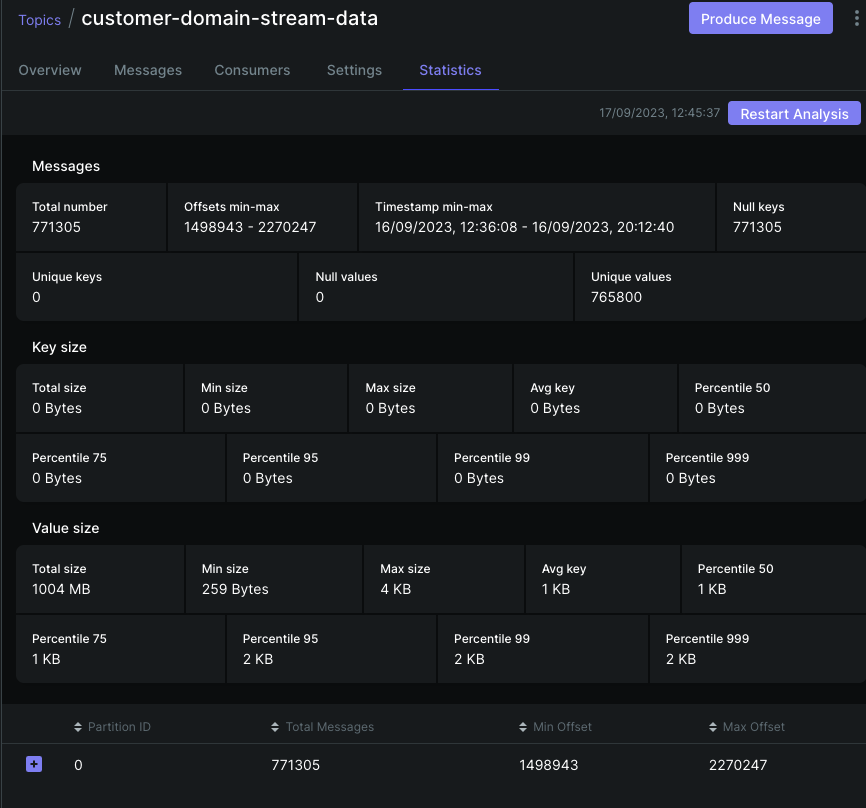
\includegraphics[width=\columnwidth]{images/customer-domain-stream-data-topic-statistics.png}

  \caption{Customer Domain Streaming Topic Statistics}

  \label{customerDomainStreamingTopicStatistics}

\end{figure}

\paragraph{Memory and CPU Utilisation} Memory usage is crucial in this high-speed data scenario. Regularly monitoring memory consumption was crucial in assessing the overall health and efficiency of the system. The memory usage in the customer domain reached a significant peak, measuring 12,852,592,640 bytes. The complexity of the chunking logic used in the streaming operation is the reason for this (Figure~\ref{memoryUtilizationInCustomerDomainInHighVelocityCase}). In contrast, the weather domain, which functions as the recipient of data, indicated a more conservative use of memory. This is believed to be a result of its more straightforward data processing logic, which does not include the additional steps of chunking (Figure~\ref{memoryUtilizationInWeatherDomainInHighVelocityCase}).

\begin{figure}[ht]

  \centering

  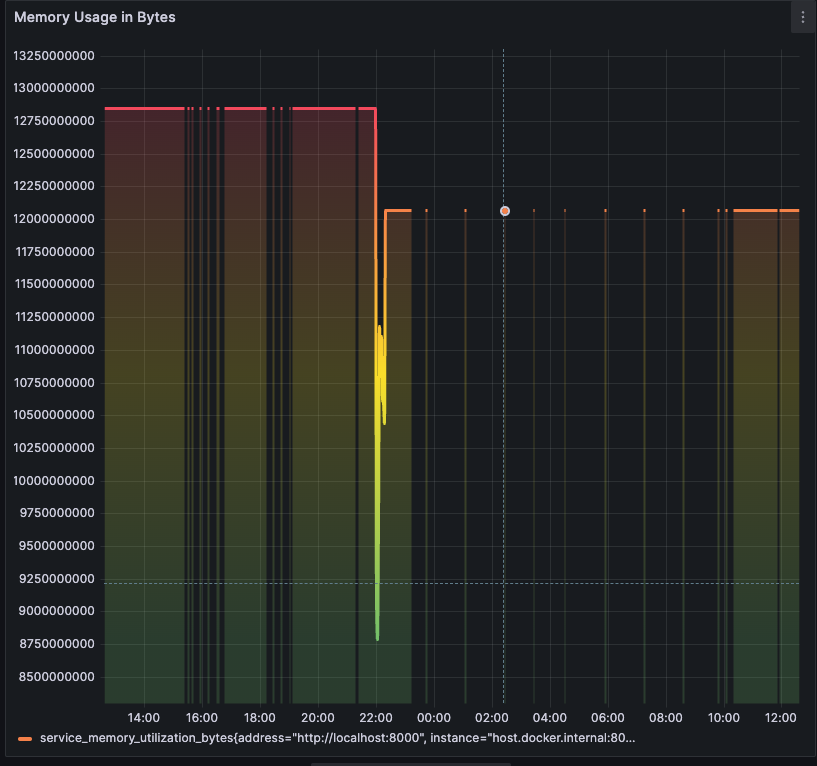
\includegraphics[width=8cm]{images/memory-utilization-in-customer-domain-in-streaming-case.png}

  \caption{Memory Utilisation in Customer Domain in High Velocity Case}

  \label{memoryUtilizationInCustomerDomainInHighVelocityCase}

\end{figure}

\begin{figure}[ht]

  \centering

  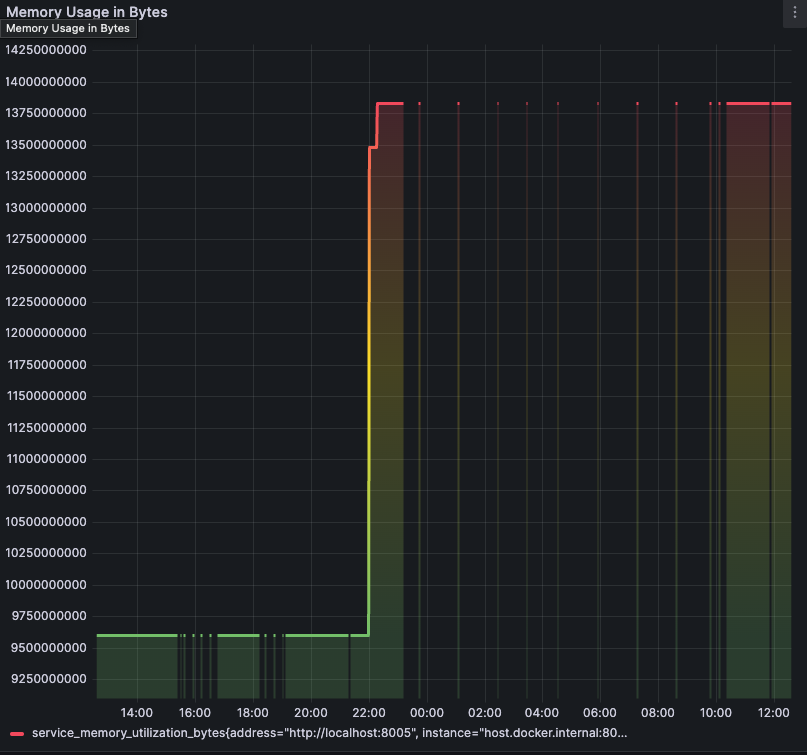
\includegraphics[width=8cm]{images/memory-utilization-in-weather-domain-in-streaming-case.png}

  \caption{Memory Utilisation in Weather Domain in High Velocity Case}

  \label{memoryUtilizationInWeatherDomainInHighVelocityCase}

\end{figure}

Furthermore, the CPU consumption has only grown by 5\% compared to the statistics mentioned in the section titled CPU Usage for both the Kubernetes cluster and its associated services. Therefore, no further data is provided for this metric.

\paragraph{Duration of Processing and Latency of Ingestion} The latency of ingestion, defined as the time delay between receiving a data packet and processing it, remained constant during the observed timeframe. The delay continuously registers a value of 0.0000148 seconds at various time intervals throughout the monitoring period. This observation suggests that the system's data ingestion mechanism does not experience substantial delays in processing. However, a more comprehensive evaluation can be obtained by comparing its performance benchmarks with those of other platforms (Figure~\ref{kafkaIngestionLatencyInStreamingCase}). The system's ability to maintain consistent latency indicates its capacity to sustain performance levels without interruption, especially during periods of heavy data flow.

\begin{figure*}

  \centering

  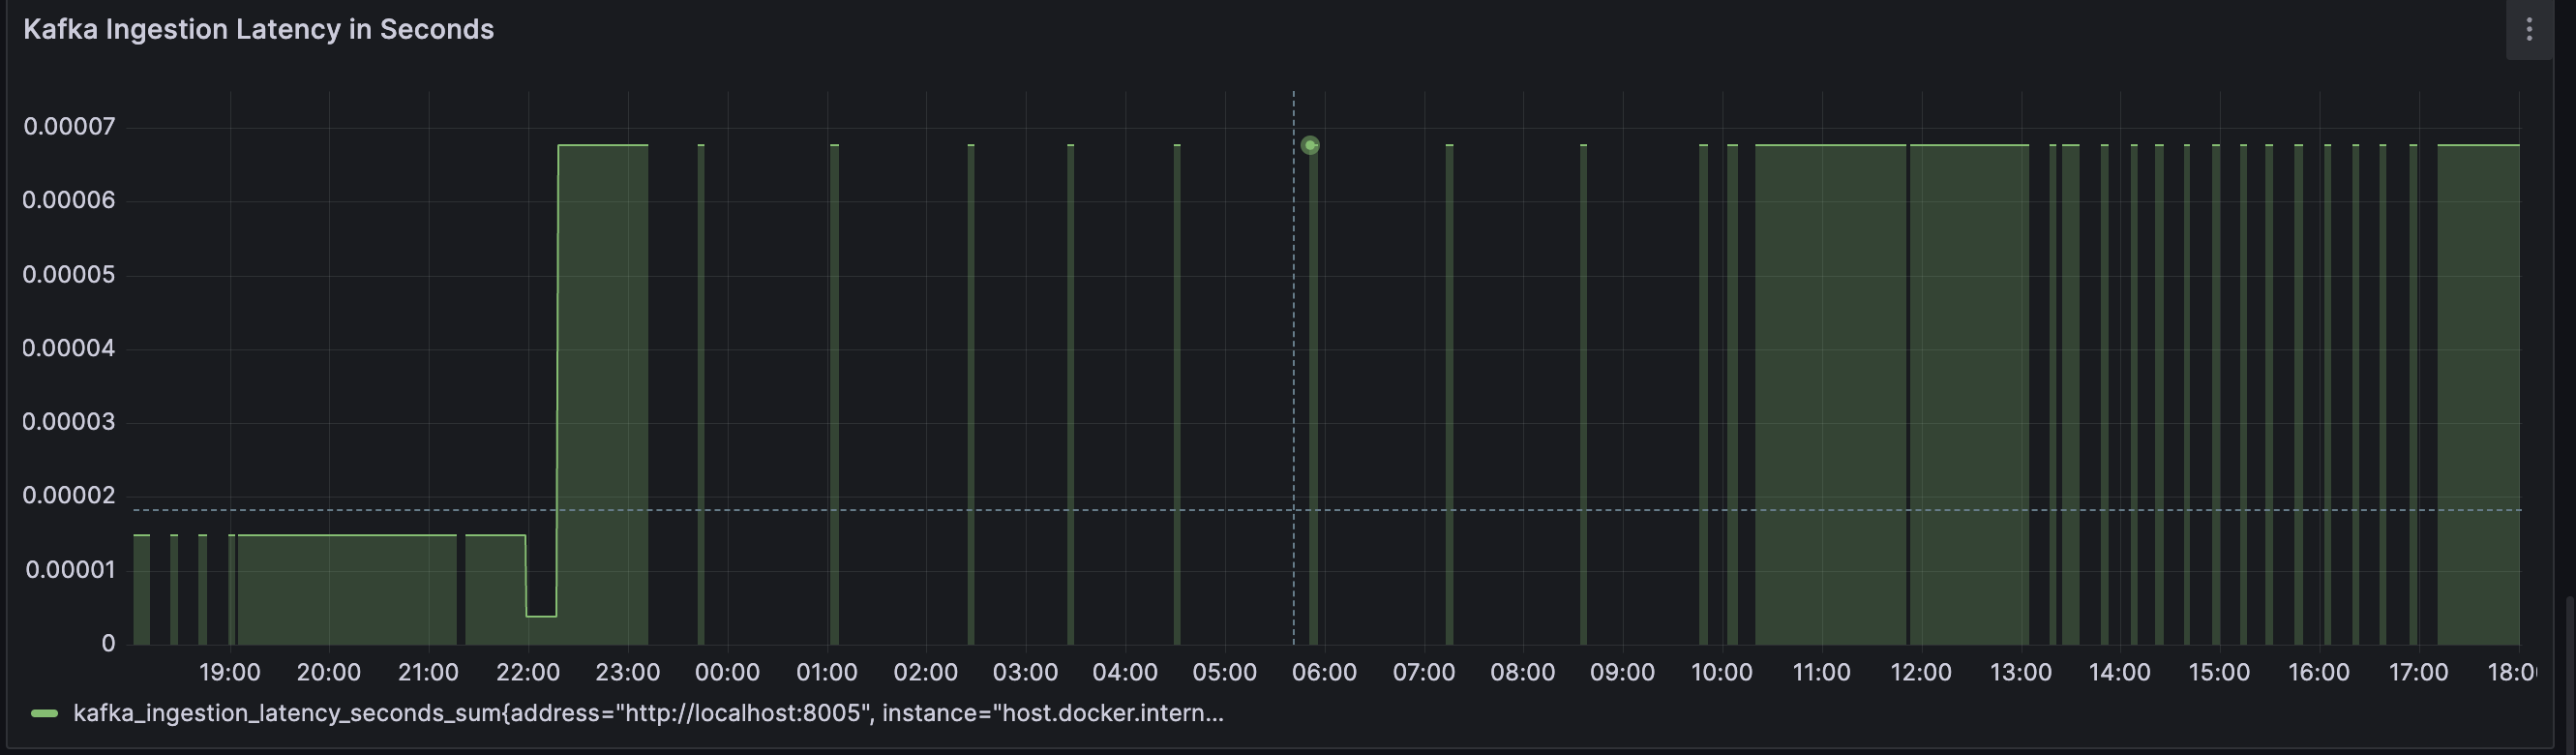
\includegraphics[width=\textwidth]{images/kafka-ingestion-latency-sum-streaming-case.png}

  \caption{Kafka Ingestion Latency in Streaming Case}

  \label{kafkaIngestionLatencyInStreamingCase}

\end{figure*}

Furthermore, the processing duration provides us with information on the amount of time it takes for the system to process the data that has been received. The Weather Domain consistently processes data in 1,694,491,558 nanoseconds (or approximately 1.6945 seconds) for various timestamps (Figure~\ref{processingDurationInStreamingCaseInWeatherDomain}). The consistency seen suggests a reliable data processing method that remains unaffected by any potential variables encountered during the streaming process.

\begin{figure*}

  \centering

  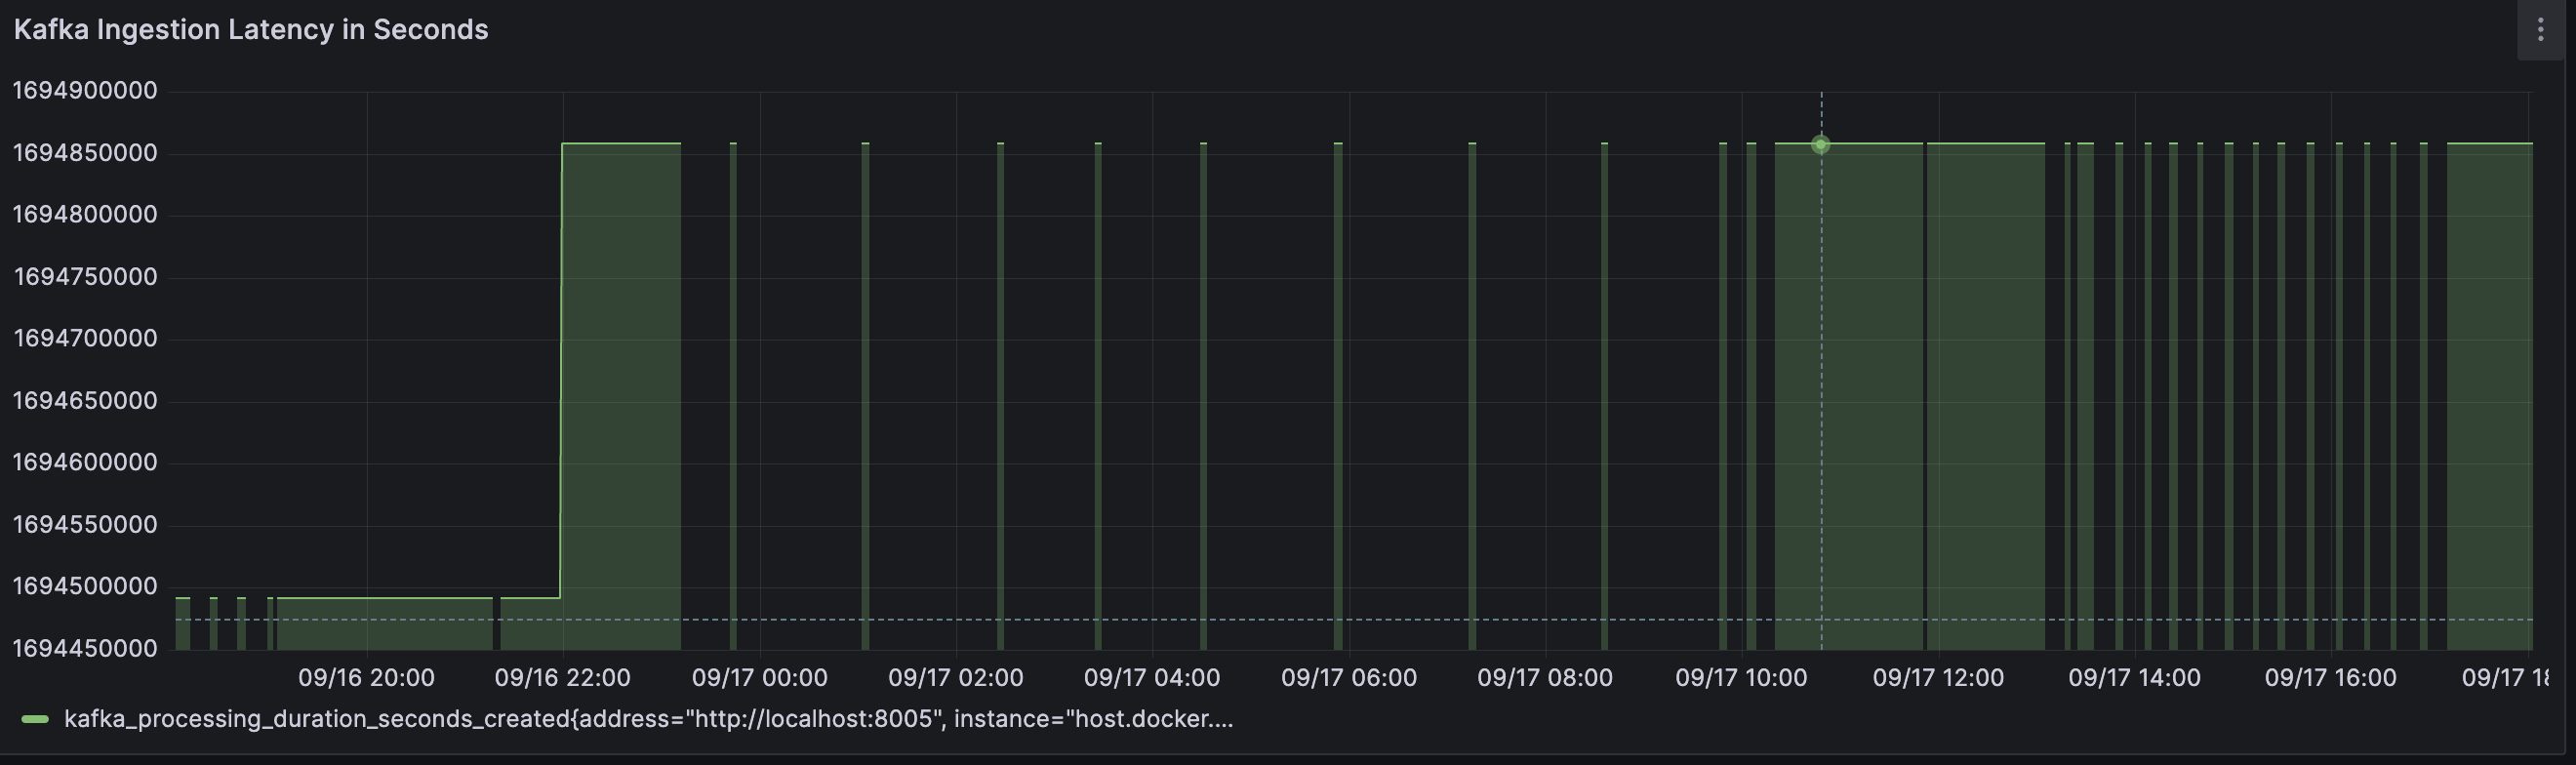
\includegraphics[width=\textwidth]{images/processing-duration-streaming-case-in-weather-domain.png}

  \caption{Processing Duration in Streaming Case in the Weather Domain}

  \label{processingDurationInStreamingCaseInWeatherDomain}

\end{figure*}

The assessment of the High Velocity Data Intake Scenario (S2) demonstrated that the system consistently handled the rapid intake of data within the specified parameters, indicating its effective capability to manage such scenarios. By establishing a specialised Kafka topic and strategically integrating a new endpoint in the customer domain to enable data streaming, we are able to accurately replicate peak data input rates. The system's memory use patterns demonstrate its ability to handle large amounts of data. More precisely, the consumer domain, influenced by its chunking logic, exhibits more memory consumption in comparison to the weather domain. However, both domains efficiently managed the processing and intake of a significant total of 771,305 messages (about 1GB in size). 

Moreover, the continuous delay in consuming data and the time taken for processing highlight the system's resilience. Overall, the system effectively showcases its ability to handle a constant flow of fast-moving data without any noticeable decrease in performance, fulfilling the anticipated results of Scenario S2. Furthermore, the system has been continuously checked to guarantee that the allocated memory for streaming is released after the transmission is finished. No memory leak was detected during the monitoring process, and all memory was successfully released after the streaming was completed.

Based on the extensive results obtained from Scenarios S1 and S2, which include both high-volume and high-velocity data ingestion processes, it is concluded that Scenario S3's emphasis on data variety is inherently resolved and confirmed, eliminating the need for a separate testing phase for Scenario S3.

\subsubsection{Scenario S4, S5, S6}

Subsequently, an evaluation is conducted for Scenarios S4, S5, and S6 as a whole. The decision to test these scenarios concurrently is based on the fact that they have common system operations and the capacity to provide a thorough system evaluation while maximising efficiency. Furthermore, the interconnected relationship between OpenID Connect and bearer token systems implies that doing a simultaneous test would provide a comprehensive understanding of the system's performance.

A Python service is initialised to replicate the behaviour and workload of an external data scientist. While Jupyter Notebook was originally designed to replicate the tasks performed by data scientists, a separate Python service has emerged as the best option. Its inherent low-level characteristics allow for precise management and enhance the efficiency of capturing metrics. Similar to previous services, this Python service is equipped to provide telemetry data to a telemetry processing application via Kafka REST proxy. 

Keycloak, the authentication and authorization server, plays a crucial role in this ecosystem. Upon initiation, the Python service acquires authorization by creating a client in Keycloak. The following confidential information, crucial for the functioning of the service, is securely stored in and retrieved from the HashiCorp Vault. 

The authentication process, enabled by OpenID Connect standards, allows the simulated data scientist to effortlessly access Data Lichen. After being registered, the data scientist can access and see datasets from many domains. They can then send network requests to retrieve the specific data they need. The flow is illustrated in Figure~\ref{dataScientistFlowWithAuthentication}.

\begin{figure*}[ht]

  \centering

  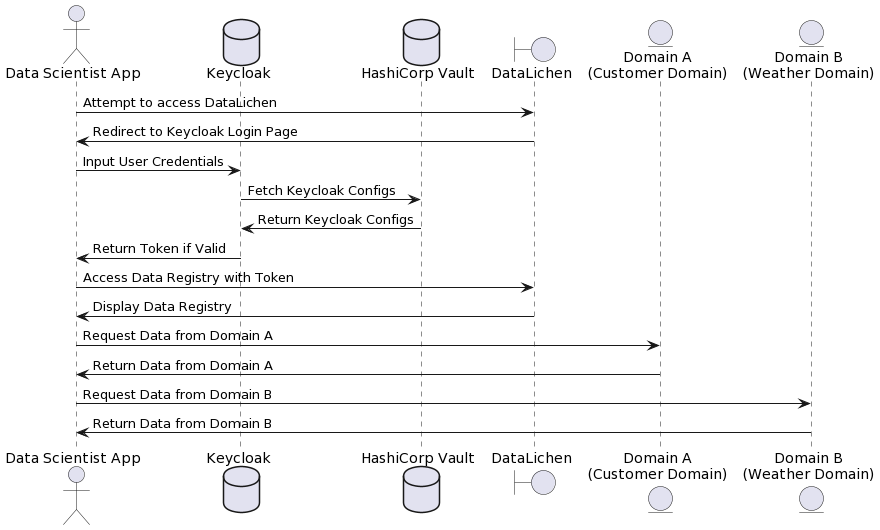
\includegraphics[width=\textwidth]{images/data-scientist-data-lichen-flow-with-authentication.jpg}

  \caption{Data Scientist Flow with Authentication}

  \label{dataScientistFlowWithAuthentication}

\end{figure*}

It is noteworthy that the Minio secret key and access key could also be stored in the vault and retrieved in each service; nevertheless, this is not done due to time and resource constraints. This does not risk the integrity of this experiment. For scenarios S4, S5, and S6, the metrics below are selected: 

\begin{enumerate}

  \item \textbf{Query Processing Time (QPT):} Measures the duration from when a complex query is initiated to when its results are returned. It encapsulates computational efficiency and performance.

  \begin{equation}
      QPT = t_{query completed} - t_{query initiated}
  \end{equation}

  \item \textbf{Secret Retrieval Latency (SRL):} Captures the time taken to retrieve secrets. It summarises the system's efficiency in secret management.

  \begin{equation}
      SRL = t_{secret retrieved} - t_{retrieval initiated}
  \end{equation}

  \item \textbf{Data Integrity Verification (DIV):} Assesses the integrity of data during transmission and processing, ensuring data security.

  \begin{equation}
      DIV = Hash(Data Sent) \stackrel{?}{=} Hash(Data Received)
  \end{equation}

\end{enumerate}

After obtaining the domain data using a secure method utilising OpenID Connect and Vault on many occasions and over various days, the following conclusions arise:

\paragraph{Duration of Secret Retrieval:}

The recorded metrics consistently displayed a length of 3 seconds throughout the timestamps. This demonstrates a dependable and consistent secret management system, as depicted in Figure~\ref{dataScientistSecretRetrievalDelayInSeconds}.

\begin{figure*}[ht]

  \centering

  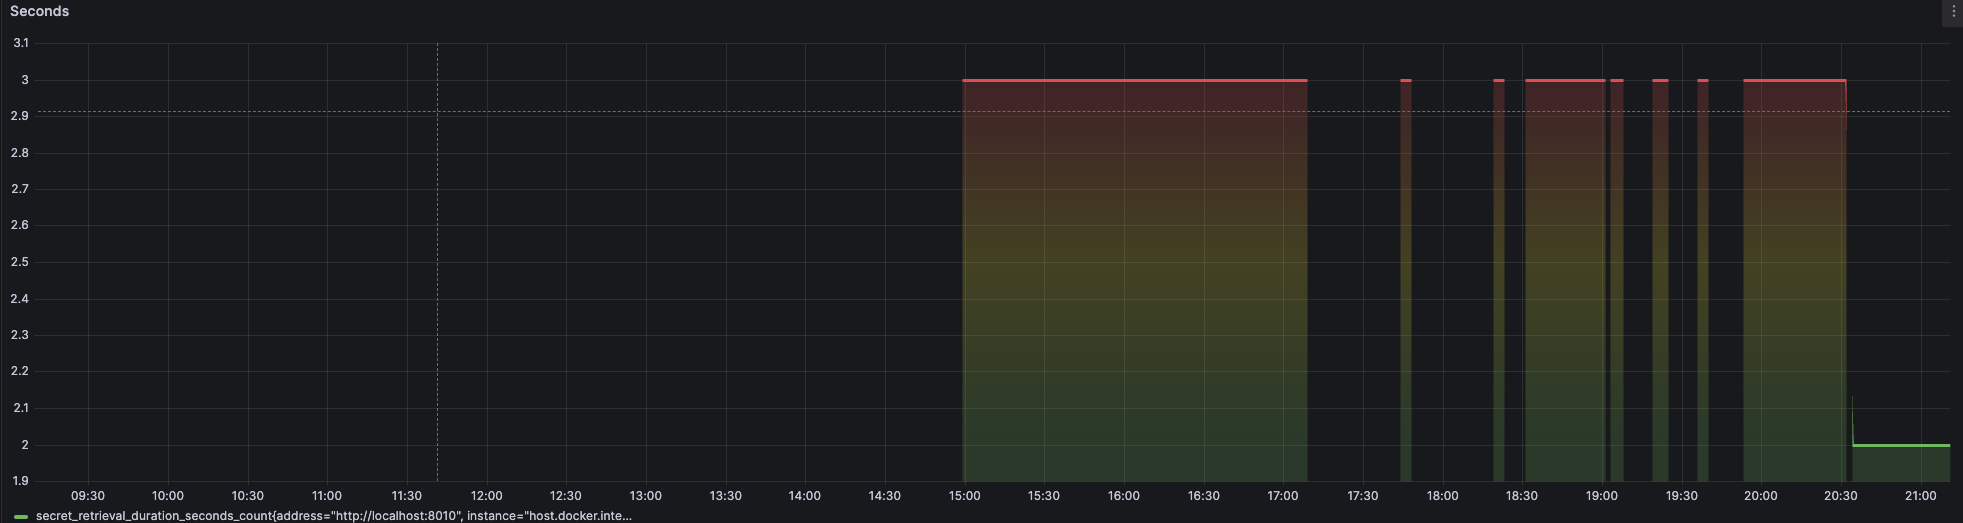
\includegraphics[width=\textwidth]{images/Secret-Retrieval-Delay-in-Seconds-In-Data-Scientist-Application.png}

  \caption{Data Scientist Secret Retrieval Delay in Seconds }

  \label{dataScientistSecretRetrievalDelayInSeconds}

\end{figure*}

The CPU utilisation remains constant at 18.6\% during the recorded time period. The behaviour can be linked to the special resource allocation of the operating system on the Apple M2 chip, which enables a consistent usage of the central processing unit (CPU), as shown in Figure~\ref{cpuUtilizationInDataScientistApplication}. As a result, CPU consumption may change in various circumstances.

\begin{figure*}[ht]

  \centering

  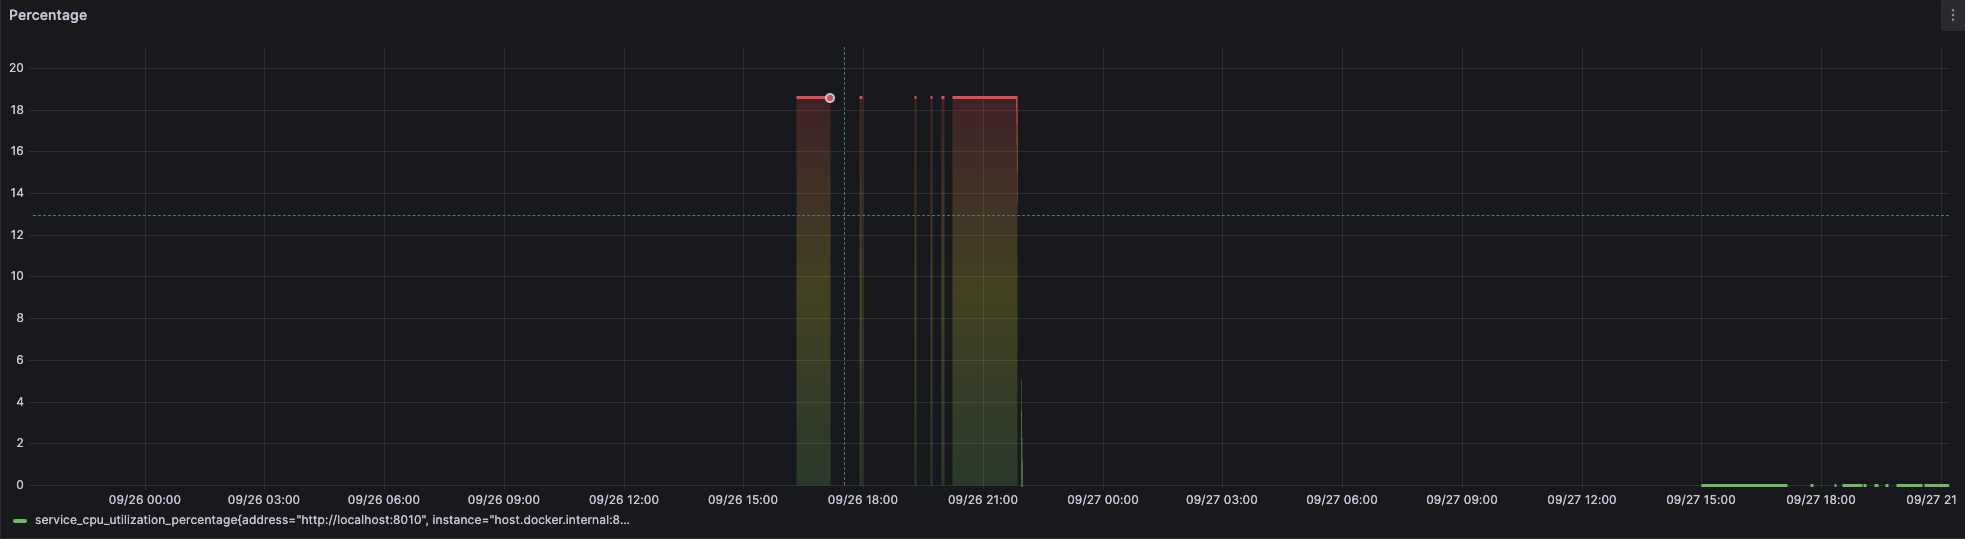
\includegraphics[width=\textwidth]{images/CPU-utilization-data-scientist-application.png}

  \caption{CPU Utilization in Data Scientist Application}

  \label{cpuUtilizationInDataScientistApplication}

\end{figure*}

\paragraph{Memory Utilisation in the Data Scientist Application:}

The memory utilisation remains consistently at around 12.56 GB during all observations. This suggests that the application possesses efficient memory management and does not encounter memory leaks or substantial variations. This is illustrated in Figure~\ref{memoryUtilizationInDataScientistApplication}.

\begin{figure*}[ht]

  \centering

  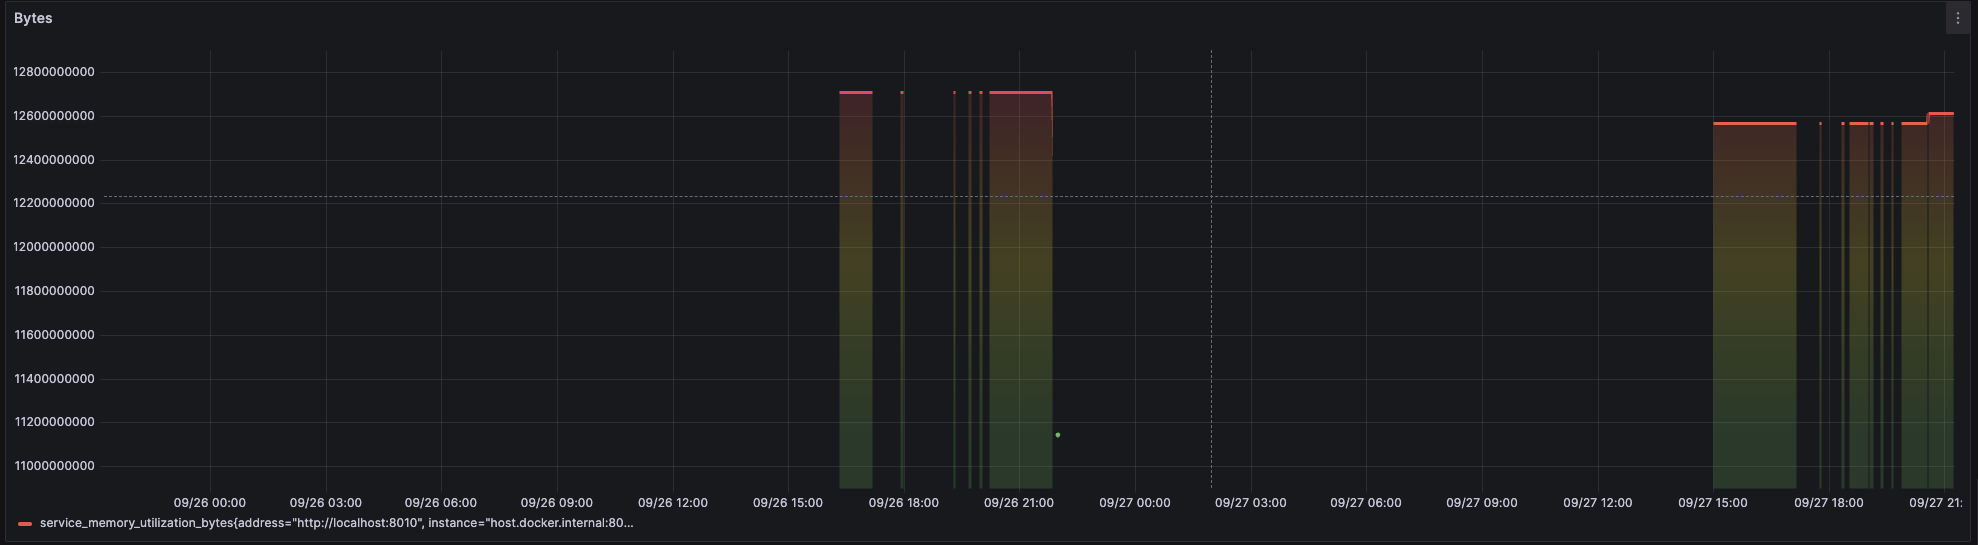
\includegraphics[width=\textwidth]{images/memory-utilization-in-data-scientist-application.png}

  \caption{Memory Utilization in Data Scientist Application}

  \label{memoryUtilizationInDataScientistApplication}

\end{figure*}

\paragraph{Query Processing Duration}

The duration of query processing consistently stayed at 10 seconds throughout the measured time period. Nevertheless, there is a decrease to 2 seconds at the conclusion of the observation period (Figure~\ref{queryProcessingDurationInDataScienceApplication}). This abrupt decline indicates potential opportunities for optimising or modifying the characteristics of the processed queries.

\begin{figure*}[ht]

  \centering

  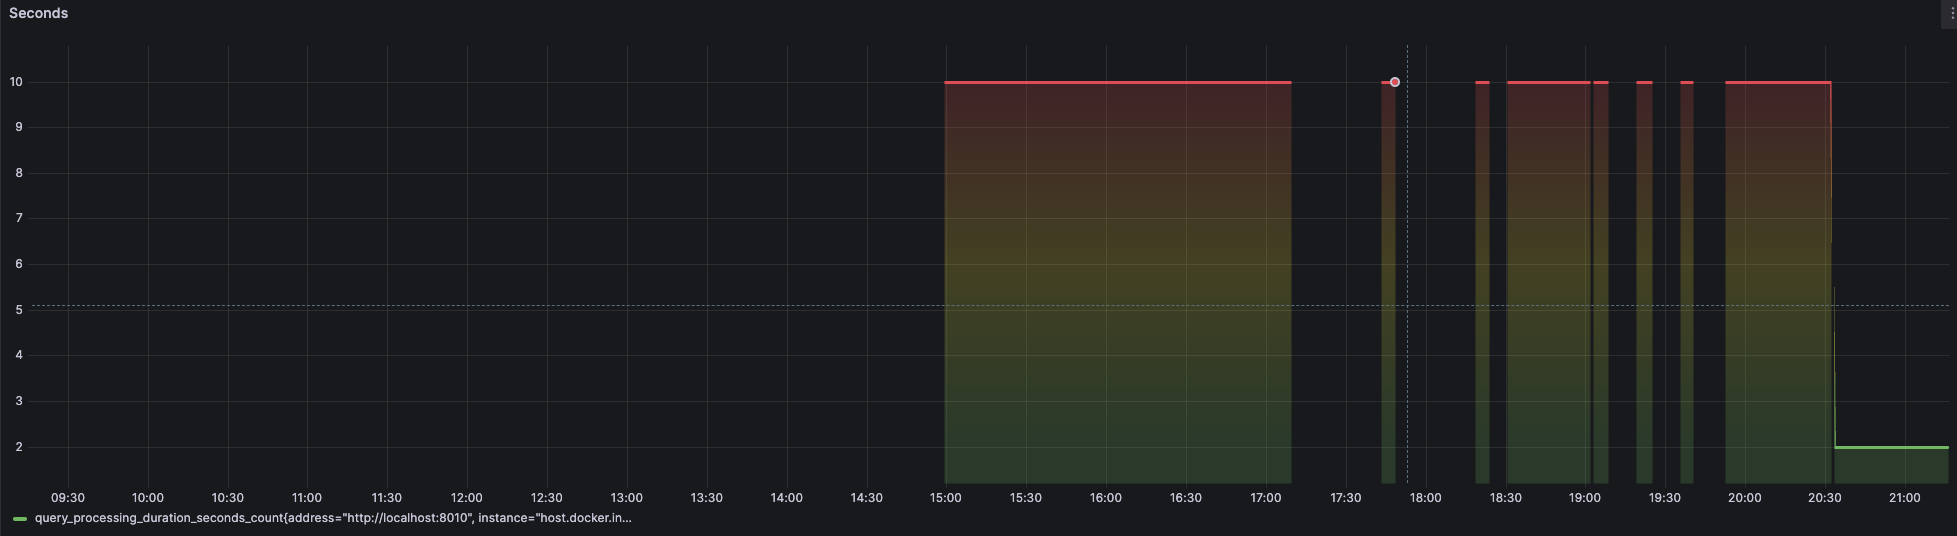
\includegraphics[width=\textwidth]{images/query-processing-duration-in-data-science-application.png}

  \caption{Query Processing Duration in Data Science Application}

  \label{queryProcessingDurationInDataScienceApplication}

\end{figure*}

An essential element contributing to the system's reliable performance is its domain-driven asynchronous and event-driven architecture, which is in line with the research conducted by Braun (2021) on distributed systems. This architecture demonstrates good proficiency in handling simultaneous data access and ensuring the integrity of domain models in asynchronous scenarios, concepts that are also discussed in Kleppmann's renowned book, "Designing Data-Intensive Applications" (2017). The prototype's capacity to manage simultaneous updates and uphold data integrity demonstrates the effectiveness of this architectural approach in the construction of distributed systems.

\subsection{Challenges and Duration of the Experiment}

The experimentation phase lasts around four months and involves a methodical process to assess each situation in order to thoroughly validate the Terramycelium system according to the specified specifications. The experiment faced numerous architectural and technical obstacles, which greatly influenced the design decisions and comprehension of the system's behaviour. The issues are classified into four categories: Infrastructure, Integration, Data Management, and Performance.

\subsubsection{Challenges in Infrastructure} 

\begin{enumerate}[label=({\alph*}) , leftmargin=30px]

    \item The Confluent Helm charts were incompatible because they relied on an alpha version of a Kubernetes resource called PodResourceBudget. The resource was in the alpha stage until V1.22, however, this experiment was conducted on version 1.27. The Nginx Ingress attempted to utilise the cloud manager to establish a load balancer, which led to the ingress service's external IP being stuck in a perpetual pending state. This happened because the cluster was initiated in a local development environment, resulting in the unavailability of a cloud service to deploy a load balancer such as EKS or AKS.

    \item A further infrastructure obstacle emerged with the Kafka pod, which had recurring failures. Due to Kafka's extensive use of file storage, such as segment files and log files, the initial allocation of 64GB for the Kafka instance was inadequate. Afterwards, the configuration was modified, increasing the cluster storage capacity to 300GB.

    \item During the development process, Prometheus and Grafana need a host address for the purpose of intercommunication. The same applies to both the telemetry processing service and the Prometheus metrics scraper. Nevertheless, due to the fact that the prototype was created within a solitary computational setting, a significant portion of the communication relied on the main system. This presented challenges, as the loopback address or localhost in each Docker container resolved to the container's loopback interface rather than the host's interface. In order to address this problem, a separate DNS was used that specifically pointed to the host.

\end{enumerate} 

\subsubsection{Integration Challenges} 

\begin{enumerate} [label=({\alph*}) , leftmargin=30px]

  \item An important obstacle was encountered when attempting to establish a connection between the Keycloak helm chart and the Postgres DB, despite specifically configuring a login and password. The cluster necessitated repeated restarts. The final answer entailed transitioning from Minikube to KIND.

     Once the entrance was established, the objective was to precisely route traffic to different services. The majority of services had their own dedicated servers, which required the proper configuration of the reverse proxy to ensure that upstream servers could reply effectively. For example, the Keycloak server experienced difficulties in identifying some host paths, as it expected a root path for serving files. Both the server and proxy required modifications to ensure proper functioning. Most services encountered similar problems because many open-source software needed to be configured in order to deliver their assets on paths other than the root.

    The user's text is a single item. Hosting Vault UI through an ingress encountered difficulties because Vault-UI carries out several redirections on different application paths, making rewriting or pass-through methods ineffective. This problem elicited inquiries on prominent online platforms such as StackOverflow and Vault's GitHub repository. As of February 7th, 2023, no feasible answer had become apparent. The only feasible method entailed allocating a domain to vault-ui and directing traffic through a load balancer. Nevertheless, as Vault-UI primarily served as a graphical interface for interacting with Vault and not a core architectural element, the experiment's integrity remained unaffected.

    The user's text is a single item. Despite being deployed as a helm chart, the use of Prometheus for metrics and log retrieval by Kiali made the network connection complex. Difficulties emerged as a result of intricate networking issues and the inherent service accounts of Kubernetes. Understanding the external authorizer API used by Envoy and enabling it in a Kubernetes cluster's service mesh within a specified namespace was not easy. There was widespread confusion over the lifecycle of service mesh objects, the admission reviews, and the admission controller.

\end{enumerate}

\subsubsection{Challenges in Managing Data} 

\begin{enumerate} [label=({\alph*}) , leftmargin=30px]

    \item One of the main difficulties in designing the data quantum was figuring out the precise nature of the data resolution provided by the analytical service. Using FastAPI, which is inherently event-driven, it is not advisable to block the main thread by making continuous requests to an HTTP endpoint for events. A solution utilised a function that was executed conditionally to retrieve all events related to a certain topic, either at the system's initialization or through an endpoint.

     Another problem connected to the creation of the local-host-based cluster came in the context of ingress. In order to route incoming traffic to the Kafka REST proxy, nginx was configured to perform target rewriting. While this method is suitable for incoming network requests, outgoing requests present challenges. For instance, when the Kafka REST proxy API provided the consumer URL, it excluded the rewriting rules, which required the use of custom code to alter the URL.

     Handling the data flow for domain B, specifically the customer reviews domain, presented difficulties because of the substantial size of the Yelp academic datasets, with some reaching up to 5GB. In order to provide version control and avoid server and stream timeouts, it was necessary to divide these JSON files into smaller chunks. A bespoke Python script was created to manage the division of JSON files into smaller chunks, guaranteeing that no file surpassed 99MB.

    \item SQLite, used in analytical services to store many types of data, presented difficulties with semi-structured data such as JSON. The lack of uniformity in JSON data formats within the customer domain required the development of separate tables to accommodate various semi-structured data sets. In order to address this issue, a bespoke function was created to dynamically generate SQLite tables.

     A noticeable inefficiency arose when initially gathering metrics from different services using normal Python and Node APIs. It was quickly determined that many traces were missing important metadata, such as service name, service version, and environment, which are necessary for proper visualisation. This mistake required a repetition of the first scenario in order to provide the best possible visualisation and narrative consistency.

    An associated matter pertained to the automated removal of outdated Kafka consumers by the Kafka-rest-proxy service. As a consequence of this activity, there was a failure in the service when making further queries to Kafka. In order to alleviate this issue, a bespoke function was created to modify the consumer and restore a connection to the REST server.

\end{enumerate}

\subsubsection{Performance Challenges} 

\begin{enumerate} [label=({\alph*}) , leftmargin=30px]

    \item While transferring operational data from the operational service to the analytical service, storage information was sent along with the success event. This strategy presented causality concerns. The following queries, which were intended to process this data and record it in Datalichen, relied on the distributed storage data. To tackle this issue, it was necessary to take into account a centralised configuration pattern.

    The user's text is a single item. The Apple M2 chip architecture presented an extra performance difficulty by hindering Psutil's ability to accurately represent CPU utilisation.

\end{enumerate}

Notwithstanding these challenges, the system exhibits proficiency in managing intricate settings. Nevertheless, the scarcity of time and infrastructure constrains the extent of testing. The selected situations offer a thorough comprehension of the system's capabilities, but a more exhaustive examination is possible under more advantageous circumstances. Despite its limitations, the experiment demonstrates the resilience and promise of the Terramycelium prototype.

\subsection{Final Notes on Experiment}

The comprehensive evaluation of the Terramycelium system across several scenarios has definitively demonstrated its ability to fulfil, and in some cases, go beyond, the specified criteria. The experimental data lead to the following conclusions:

\begin{enumerate} 

  

  \item \textbf{Volume}: The large volume data import scenario, also known as Scenario S1, showcases the system's ability to handle both asynchronous and batch processing, hence fulfilling the requirements outlined in Vol-1 and Vol-2. The system offers a flexible storage solution for extensive datasets, efficiently managing the influx of data during periods of high demand.

    

    \item \textbf{Velocity}: In Scenario S2, which focused on fast data ingestion, the system demonstrated its ability to handle various data transmission speeds, satisfying requirements textbfVel-1 to textbfVel-5. The system's ability to efficiently deliver streaming data to users, along with its capacity for rapid search and real-time data processing, is very commendable.

    

    \item \textbf{Diversity}: While Scenario S3 is not explicitly evaluated, insights from Scenarios S1 and S2 strongly indicate the system's capacity to handle a wide range of data forms, ranging from structured to unstructured data. This substantiates the assertions made by Var-1 to Var-4. The system's inherent ability to gather, standardise, and adapt its structure to changing needs is a notable advantage.

    

    \item \textbf{Value}: The Complex Query Scenario (Scenario S4) demonstrates the system's computing capabilities, confirming the criteria outlined in \textbf{Val-1} to \textbf{Val-4}. The system's versatility in facilitating both batch and streaming analytical processing, as well as its adaptability in managing various output formats, distinguishes it from others. This distinction is emphasised throughout the experiment, as each domain contains a unique form of semi-structured data.

    

    \item \textbf{Security \& Privacy}: Scenarios S5 and S6 thoroughly demonstrate the system's commitment to fulfilling SaP-1 and SaP-2 by focusing on secret management and data security, respectively. By strategically using OpenID Connect with Hashicorp Vault, the highest standard of security, data preservation, and multi-tier authentication systems are ensured.

    

    \item \textbf{Veracity}: The domain-specific character of Terramycelium naturally supports the fulfilment of requirements \textbf{Ver-1} and \textbf{Ver-2}, emphasising the significance of ensuring high-quality data and maintaining its origin and history.

  

\end{enumerate}

\subsection{Threats to Validity}

This section discusses potential threats to the validity of our study on the development and evaluation of Terramycelium, taking into account the identified challenges and limitations.

\subsection{Infrastructure and Technical Challenges}

The study encountered infrastructure challenges, including issues with Kubernetes resources, difficulties with Kafka storage, and problems related to DNS configuration for container communication. These issues highlight the potential impact of technical constraints on the prototype's performance and the generalizability of our findings.

\subsection{Integration and Data Management Difficulties}

Integration challenges with third-party services like Keycloak and the management of large datasets underscore the complexities of building BD systems. These difficulties reflect on the RA's adaptability and its applicability across different domains and data scales.

\subsection{External Validity}

The experimental design, focusing on a prototype and selected scenarios for RA evaluation, may not cover the breadth of potential real-world applications. This limitation could affect the generalizability of our findings to other contexts or systems with different requirements.

Addressing these threats to validity involves further research, particularly exploring alternative technologies, expanding the experimental design to cover a wider range of scenarios, and conducting comprehensive performance and scalability testing.

\subsection{Construct Validity}

Construct validity is a cornerstone of our research methodology, particularly in ensuring that Terramycelium accurately reflects and addresses the multifaceted nature of BD systems. To this end, we have undertaken several critical steps:

\begin{enumerate}

    \item We meticulously align the operational definitions of key BD characteristics -- including velocity, veracity, volume, variety, value, security, and privacy -- with the constructs integrated into the Terramycelium RA. This alignment is essential to mitigate ambiguity and uphold the RA's construct validity \cite{rad2017big}.

    

    

    \item Validation of the RA against established best practices and industry standards is undertaken rigorously. Such an alignment is crucial for ensuring that the RA adheres to widely recognised norms and practices, a key aspect of construct validity.

    

    \item Lastly, we assess the adaptability and scalability of Terramycelium in response to evolving data needs and varying workloads. This evaluation demonstrates the RA's flexibility and robustness, underscoring its long-term relevance and thereby enhancing construct validity in dynamic BD environments.

\end{enumerate}

% \section{Evaluation 2: Expert Opinion}

% In the preceding section, a prototype of Terramycelium is fabricated and exposed to several simulations. Expert review is used as the second evaluation approach for the artefact. In order to acquire expert opinions, the research technique adheres to the standards set forth by Kallio (2016) in their systematic study.

% \subsection{Research methodology for gathering expert opinion}

% The research methodology for soliciting expert feedback comprised five stages: \begin{enumerate}[label=\alph*)]

%   \item Rationalizing the need for expert opinion

%   \item Developing a preliminary guide

%   \item Designing a rigorous data collection method

%   \item Pilot testing the guide

%   \item Presenting the results

%   \end{enumerate}

  

%   Given the study's architectural focus, expert feedback was deemed an appropriate approach \citep{creswell2007qualitative}. In a novel domain, erudite perspectives could offer invaluable insights and enhance the theoretical underpinnings' robustness.

  

%   \subsubsection{Rationale for Expert Opinion}

  

%   The intricacy of a domain-driven distributed reference architecture for big data necessitated an evaluation transcending theoretical confines. Experts possess an unparalleled depth of knowledge, enabling them to assess practical relevance, identify oversights, and ensure industry alignment, scalability, and benchmarking against existing solutions.

  

%   Furthermore, their detached stance served as a critical counterweight, ensuring an unbiased assessment, often lacking in internal evaluations. Seeking expert opinion was essential for a comprehensive and nuanced review, validating the architecture's robustness against diverse challenges.

  

%   \subsubsection{Developing the Guide}

  

%   The semi-structured protocol for expert opinion is inspired by the works of Kallio et al. \cite{kallio2016systematic}. This protocol is aimed at extracting expert opinion while ensuring participant-centricity. Close-ended questions facilitated quantifiable data extraction and conversation initiation.

  

%   The guide was segmented into main themes and ancillary follow-up questions, adhering to a logical trajectory.

  

%   \subsubsection{Data Collection Method}

  

%   Purposive sampling identified experts, providing in-depth insights through targeted selection \cite{baltes2022sampling}. Contacts were initiated with professionals in relevant roles, such as data engineers, data architects, chief data and analytics offers, solution engineers, solution architects, principal data engineers, staff data engineers, principal architectures, and scholars and researchers whose work is in BD systems. Over two months, three experts across different sectors were selected, as displayed in Table~\ref{tab:experts}.

%     \begin{table}[htbp]

%     \centering

%     \caption{Participant Demographics}

%     \label{tab:experts}

%     \begin{tabular}{llll}

%     \hline

%     Expert & Role & Experience & Industry \\

%     \hline

%     i1 & Solution Engineer & 10 years & Software Development \\

%     i2 & Solution Architect & 11 years & Big Data Solutions \\

%     i3 & Principal Architect & 32 years & Biotechnology Research \\

%     \hline

%     \end{tabular}

%   \end{table}

    

  

%   Expert opinions were collected via Zoom. Transcripts were reviewed, rectified, and coded in NVivo based on predefined themes, including 'Applicability \& Industrial Relevance', 'Strengths \& Distinctive Features', and 'Challenges \& Potential Barriers'.

  

%   \subsubsection{Pilot Testing}

  

%   The guide underwent internal peer review and an empirical pilot study with other researchers to diagnose incongruities, refine ancillary questions, and calibrate the discourse trajectory. This iterative refinement accentuated the study's rigour.

% \subsection{Thematic Analysis} \label{expertOpinion_thematicAnalysis}

% This section systematically identifies and analyses prominent topics seen in expert comments. This examination not only emphasises reoccurring concepts but also places the range of viewpoints that shape the artefact's structure into its proper context.

% \subsubsection{Applicability \& Industrial Relevance}

% The domain-driven and distributed nature of the Terramycelium architecture elicits various viewpoints regarding its compatibility with existing industry practices and anticipated future developments. Although this architectural approach incorporates promising and advanced approaches, it is clear that they are not uniformly embraced in all industries.

% i2 suggested that the utilisation of Terramycelium could be impacted by team configurations and the scale of the organisation. In addition, there was evidence suggesting that different practices may have a higher level of proficiency in specific data practices, with only a small proportion adopting sophisticated approaches such as microservices or streaming.

% \,

% \setlength{\fboxsep}{0.3em}

% \noindent\fbox{%

% \parbox{\columnwidth}{%

% \textit{"In certain areas, the sense is of being slightly ahead of times, with only a few diving into micro services."} - i2

% }%

% }

% \,

% i1 highlighted the architecture's ability to handle eventing, data streaming, and batch processing. However, there were remarks made regarding possible discrepancies between current industry trends and specific aspects of the architecture.

% \,

% \setlength{\fboxsep}{0.3em}

% \noindent\fbox{%

% \parbox{\columnwidth}{%

% \textit{"Industry trends might not align perfectly, but this is definitely industry relevant."} - i1

% }%

% }

% \,

% The i3 stated that the architecture's domain-driven nature was very remarkable. As industries move towards greater granularity and distribution of data ownership, they face obstacles. In addition, i3 expressed concerns about the intricate structure of this technique, indicating that its complexity could provide difficulties in its implementation.

% \,

% \setlength{\fboxsep}{0.3em}

% \noindent\fbox{%

% \parbox{\columnwidth}{%

% \textit{"The architecture's complexity might challenge some organisations, even larger ones, during adoption."} - i3

% }%

% }

% \,

% Considering the opinions of specialists, it is clear that Terramycelium provides promising opportunities for many sophisticated data operations. Nevertheless, the originality and intricacy of the subject could be both advantageous and challenging. It may appeal to organisations seeking new solutions, but it could also be perceived as intimidating by those accustomed to more conventional approaches or those who are not yet ready for such a significant change in their data practices.

% Overall, the design of the Terramycelium architecture shows great potential. However, its deviation from conventional approaches may be seen as a possible obstacle to wider acceptance. The difficulty lies in synchronising its sophisticated characteristics with the existing level of preparedness and environment in the industry.

% \subsubsection{Strengths \& Distinctive Features}

% The Terramycelium architecture received praise for its unique characteristics and apparent advantages, especially in terms of incorporating domain-driven design into data engineering.

% i1 emphasised the value of using a domain-driven strategy in conjunction with data engineering. Recognising the historical separation between software engineering and data engineering in terms of their objectives and key performance indicators (KPIs), they highlighted the importance of closing this gap.

% \,

% \setlength{\fboxsep}{0.3em}

% \noindent\fbox{%

% \parbox{\columnwidth}{%

% \textit{"Most of the time you were talking, you were putting software engineering and data engineering together. It sounds really good in theory... If you manage to solve that, that could be a good strength to have... teams working together, you don't have a person in the middle, so you can move much faster."} - i1

% }%

% }

% \,

% This integration was also recognised as a novel approach by i2, who added:

% \,

% \setlength{\fboxsep}{0.3em}

% \noindent\fbox{%

% \parbox{\columnwidth}{%

% \textit{"I like that. That will be quite distinctive, because I'm yet to see that in action."} - i2

% }%

% }

% \,

% The architecture's adaptable characteristics and all-encompassing ecosystem also garnered favourable recognition. i3 mentioned that the architecture seems to be effective for its capacity to handle a wide range of tasks, including batch eventing and stream processing. I3 also emphasised the importance of maintaining immutable logs, which ensures a reliable and authoritative source of information. This expert highlighted the importance of data dimensions such as bitemporality and immutability. 

% \,

% \setlength{\fboxsep}{0.3em}

% \noindent\fbox{%

% \parbox{\columnwidth}{%

% \textit{"It considers everything from batch eventing, ACLs. Immutable log is very important these days because it helps identify the single source of truth."} - i3

% }%

% }

% \,

% Moreover, the architecture's ability to promote the idea of a platform as a service was considered essential.

% \,

% \setlength{\fboxsep}{0.3em}

% \noindent\fbox{%

% \parbox{\columnwidth}{%

% \textit{"As a platform as a service, the fact that you can self provision components as you need to is very important."} - i3

% }%

% }

% \,

% The modular architecture was emphasised by i2, which also emphasised the benefits of having distinct boundaries between various components, including data governance, domain-driven design, and data ingestion.

% \,

% \setlength{\fboxsep}{0.3em}

% \noindent\fbox{%

% \parbox{\columnwidth}{%

% \textit{"I love this modular approach... I love the fact that it also calls out domain driven design and a clear separation of data governance."} - i2

% }%

% }

% \,

% Aside from discussing how it differs from other methods and recognising its distinct position, i1 also explored how it combines various data views, such as data mesh and event-driven features.

% \,

% \setlength{\fboxsep}{0.3em}

% \noindent\fbox{%

% \parbox{\columnwidth}{%

% \textit{"I think bits and pieces come from a different view. Like you have a data mesh here, event-driven there... The approach of an open policy agent looks promising."} - i1

% }%

% }

% \,

% In wrapping up, the overall sentiment suggests that while certain components of Terramycelium might find parallels in the industry, its holistic approach and integration of domain-driven design with data engineering make it a unique offering. The challenge, however, remains in ensuring this distinctiveness translates into practical advantages in the evolving landscape of data operations.

% \subsubsection{Challenges \& Potential Barriers}

% A number of specialists offered their perspectives on possible difficulties and obstacles for the Terramycelium framework. The worries revolve around many difficulties like the availability of skillsets, the inherent challenges of data governance, and concerns related to scalability.

% i1 have found a significant issue involving the necessary competence to effectively utilise the architecture, particularly at the local level.

% \,

% \setlength{\fboxsep}{0.3em}

% \noindent\fbox{%

% \parbox{\columnwidth}{%

% \textit{"Skill set, that would be the biggest challenge. Because again, there would be very few data engineers who would be capable of implementing this or convincing their manager to adopt this. On the other hand, centralizing can be easy, but it is usually very hard to do well..."} - i1

% }%

% }

% \,

% The expert talked about potential political influences and the challenges of large-scale enterprise governance. This is in relation to the federated computational governance.

% \,

% \setlength{\fboxsep}{0.3em}

% \noindent\fbox{%

% \parbox{\columnwidth}{%

% \textit{"The idea of federated computational governance is outstanding! It's the architect's dream of automatic quality control. But, talking big enterprises, there's always politics in it, and not all may be open to such approach"} - i1

% }%

% }

% \,

% Additionally, i1 emphasised how crucial governance flexibility is, particularly when considering software engineering.

% \,

% \setlength{\fboxsep}{0.3em}

% \noindent\fbox{%

% \parbox{\columnwidth}{%

% \textit{"From a software engineering background... the computational governance should not affect everything a developer do everyday. In Software, it is a bit more flexible for the deloper to own a service and make several technical decisions; So this component may introduce frictions as different teams may have different KPIs which is not in-line with the federated computational governance."} - i1

% }%

% }

% \,

% i1 specifically brought up the difficulties that could develop as a result of changing ownership patterns and dependencies.

% \,

% \setlength{\fboxsep}{0.3em}

% \noindent\fbox{%

% \parbox{\columnwidth}{%

% \textit{"So one of the challenges I can see happening at some point as it evolves, is the ownership might become a bit more complicated... Now I have dependencies on A and B, I'm not aware of."} - i1

% }%

% }

% \,

% i2 elaborated on concerns related to the scale of data and domain specificity.

% \,

% \setlength{\fboxsep}{0.3em}

% \noindent\fbox{%

% \parbox{\columnwidth}{%

% \textit{"Some companies have very large data sets and so moving to a domain-driven is kind of wall sometimes if they have slightly monolithic systems... This data is just so big, so hard to play with."} - i2

% }%

% }

% \,

% He also pointed out challenges related to the centralised ownership of data domains. This comment further affirmed the challenges discussed in this study and the theories that underpinned the development of the artefact.

% \,

% \setlength{\fboxsep}{0.3em}

% \noindent\fbox{%

% \parbox{\columnwidth}{%

% \textit{"Yeah, where they already have this centralised kind of data warehouse and they don't know who owns what... and which domain should own, it because it is not clear."} - i2

% }%

% }

% \,

% A potential problem regarding the handling of unstructured data was also flagged.

% \,

% \setlength{\fboxsep}{0.3em}

% \noindent\fbox{%

% \parbox{\columnwidth}{%

% \textit{"I'm not sure how it works with things like unstructured data... But when you really get into really, really unstructured stuff, like emails or something like that, data governance just becomes crazy."} - i2

% }%

% }

% \,

% The challenge that could emerge from the architecture's cross-functionality was brought to light by i3.

% \,

% \setlength{\fboxsep}{0.3em}

% \noindent\fbox{%

% \parbox{\columnwidth}{%

% \textit{"This typically won't be owned by one team, because this is an ecosystem. You'll have database administrators, developers, infrastructure people, product people, service catalog people... I think the cross functionality of it all is what's difficult."} - i3

% }%

% }

% \,

% Additional obstacles that smaller organisations might encounter when attempting to implement the architecture were also highlighted by i3.

% \,

% \setlength{\fboxsep}{0.3em}

% \noindent\fbox{%

% \parbox{\columnwidth}{%

% \textit{"I think for small organisations, this is going to be quite possibly very difficult for them to implement. What's gonna happen is they'll just choose some cheaper version of this when you have not enough people to deliver this sort of stuff."} - i3

% }%

% }

% \,

% To summarise, although Terramycelium has certain advantages, it nevertheless faces certain difficulties. The barriers encompass a range of challenges, including the details of implementation, complexities that involve several functions, governance issues, domain-specific challenges, and the availability of necessary skillsets. To tackle these problems, it is necessary to combine strategic and technological initiatives in order to guarantee that the architecture can be widely applied and is effective.

% \subsection{Matrix of Responses} \label{expertOpinion_matrixResponses}

% The experts' perspectives on the Terramycelium architecture's applicability, strengths, and challenges are succinctly outlined in the table \ref{tab:responses}, which aggregates their responses.

% \begin{table*}[ht]

%   \centering

%   \caption{Mapping of expert responses against themes.}

%   \begin{tabular}{@{}llp{0.7\columnwidth}p{0.9\columnwidth}@{}}

%   \hline

%   Expert & Applicability & Strengths & Challenges \\

%   \hline

%   i1 & Mixed & Emphasises importance of flexibility in governance & Concerned about the skillset required, complexities of evolving ownership patterns, and large-scale enterprise politics \\

%   i2 & Positive & Cites large data handling and domain specificity & Mentions challenges of clear data domain ownership and difficulties with unstructured data \\

%   i3 & Positive & Stresses on the cross-functional nature and the ecosystem approach of the architecture & Highlights potential difficulties for smaller organisations and cross-functional challenges \\

%   \hline

%   \end{tabular}

%   \label{tab:responses}

% \end{table*}

% \subsection{Quantitative Summary} \label{expertOpinion_quantitativeSummary}

% The coding data clearly indicates that opinions and debates differed across several areas of the Terramycelium architecture. The numerical overview of these codings is presented in Table~\ref{tab:coding_summary}.

% \begin{table*}

%   \centering

%   \caption{Summary of coding references.}

%   \begin{tabular}{p{0.6\textwidth}p{0.15\textwidth}p{0.15\textwidth}}

%   \hline

%   Theme & Number of Coding References & Number of Items Coded \\

%   \hline

%   Applicability and Industrial Relevance & 9 & 3 \\

%   Alignment with Industry Trends and Future Projection & 6 & 3 \\

%   Applicability to Industry & 3 & 3 \\

%   Challenges and Potential Barriers & 9 & 3 \\

%   Adoption Challenges for Organisations & 6 & 3 \\

%   Scenarios Where The Architecture Is Not Best Fit & 3 & 2 \\

%   Other Opinions & 3 & 2 \\

%   Strength and Distinctive Features & 9 & 3 \\

%   Differentiating Components of the Architecture & 3 & 3 \\

%   Strengths of the Architecture & 6 & 3 \\

%   \hline

%   \end{tabular}

%   \label{tab:coding_summary}

%   \end{table*}

% The themes "Applicability and Industrial Relevance", "Challenges and Potential Barriers", and "Strength and Distinctive Features" had the most coding references, with 9 references apiece, indicating their importance in the expert debates.

% Within the section titled "Applicability and Industrial Relevance," the primary focus was on the "Alignment with Industry Trends and Future Projection," which was referenced six times.

% The theme "Challenges and Potential Barriers" received equal attention in both "Adoption Challenges for Organisations" and situations where the architecture may not be the most suitable choice.

% "Other Opinions," which presented supplementary perspectives and thoughts, was a less-discussed topic due to its inclusion of only 3 references. The data is depicted in Figure~\ref{fig:quantitativeSummaryForExpertOpinion}.

% \begin{figure*}[ht]

%   \centering

%   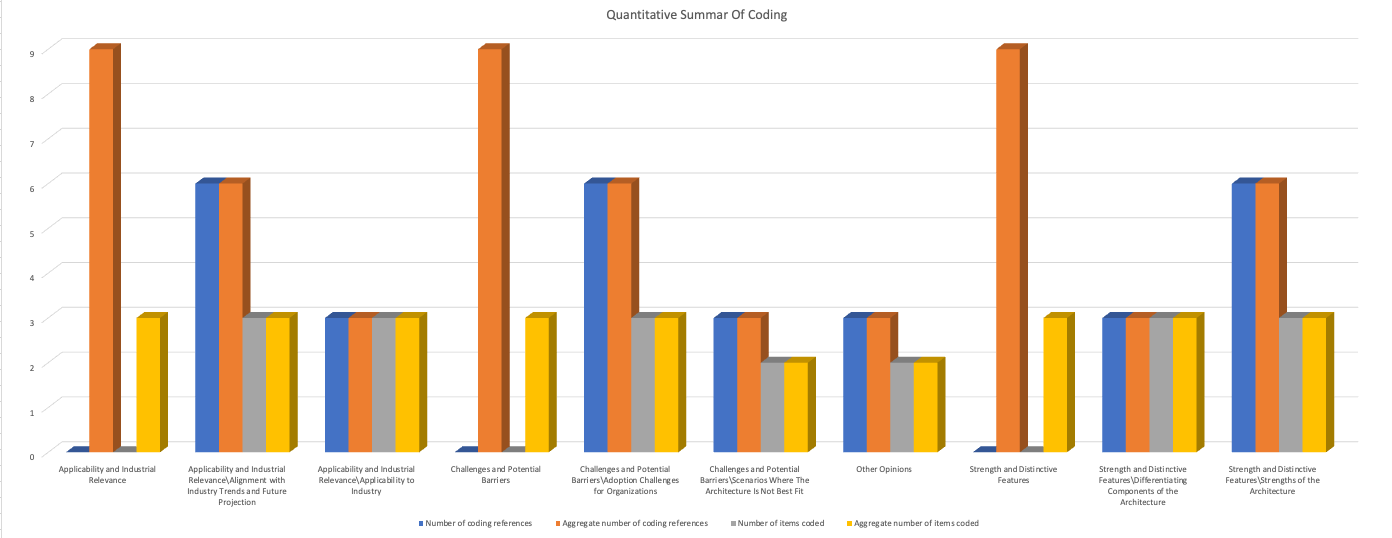
\includegraphics[width=\textwidth]{images/Quantitative-Summary-For-Codes.png}

%   \caption{Quantitative Summary For Expert Opinion}

%   \label{fig:quantitativeSummaryForExpertOpinion}

% \end{figure*}

% \subsection{Synthesis and Reflection} \label{expertOpinion_synthesisReflection}

% Experts have praised the efficiency, scalability, and effectiveness of the proposed architectural approach for handling complex operations. The architecture's ability to align with primary assumptions, handle varied scales of data, and deliver effective results in practical applications is a testament to its practical potency. However, there are areas of concern or potential limitations, such as the nascent stage of the architecture and the potential for evolution.

% Challenges like intricate data dependencies, ownership issues, and the fluid nature of data ecosystems are highlighted. Solutions like incorporating immutability and bi-temporality are discussed to address these issues. The balance between analytical and operational intents and their influence on interfacing with business processes is also explored.

% Data ownership, privacy, and governance are also discussed, with techniques like streaming between domains ensuring up-to-date data flow. The importance of customized data governance approaches and evolving governance requirements is crucial for Terramycelium's successful implementation and adoption.

% Future implications of the current reference architecture include its inherent complexity, which requires specialized skills and understanding that may not be readily accessible, particularly in organizations with limited resources or expertise. Aligning technology with human and organizational dynamics is crucial for Terramycelium's successful implementation and adoption.

% Not all organizations operate on a microservices architecture or adopt a fully domain-driven approach, as many still rely on legacy systems built with Java, PHP, and Fortran, which may not seamlessly integrate with or support the advanced paradigms proposed by Terramycelium. The complexity of Terramycelium's architecture is further intensified by the sheer number of components within its architecture, each adding to the complexity of implementation.

% The implementation of Terramycelium's comprehensive suite of components, such as IAM and secret management, presents substantial cost and time implications for organisations. To fully deploy all aspects of Terramycelium, an organization would need to invest significantly in resources and manpower, and integrate a variety of open-source technologies, which may not always have compatible interfaces. This not only extends the time and financial investment required but also necessitates a strategic approach to select and harmonize these technologies effectively within the existing organizational infrastructure.

% \subsection{Final Notes} \label{sec:finalNotes}

% The Terramycelium RA is a data management architecture that combines domain-driven design with event-driven communication, enhancing its applicability in data management challenges. It incorporates features like Data Lichen, bitemporality, and immutability, demonstrating an adaptive approach to the evolving landscape of data processing. The architecture has received positive feedback from experts, including professionals from leading data and eventing solutions companies. However, the Terramycelium faces challenges, including its complexity, which requires significant investment in skill development and training, which may be a barrier for organizations lacking resources or unwilling to undergo transformation. The lack of open-source support for components like Data Lichen adds to this challenge. The architecture's technical merits are acknowledged for its robustness and innovation, but it also requires a deep understanding of organizational culture, team dynamics, and change management strategies. The forthcoming section will analyze and synthesize the research findings, contextualizing them within the broader academic and practical landscape of BD systems.

\section{Discussion} \label{sec:discussion}

This study explored Terramycelium, a novel approach to managing the complexities of BD systems. Utilizing a complex adaptive system model, Terramycelium proposes a distributed, domain-driven architecture aiming to enhance scalability, maintainability, and adaptability beyond what traditional monolithic architectures offer. This initiative is commendable for its effort to reconcile the inherent volatility and diversity of BD with the principles of modern software engineering. However, as the following discussion highlights, the real-world applicability and scalability of such an architecture across varying domains and data scales require rigorous testing.

The initial evaluation, conducted through prototyping and case mechanism experiments, suggested potential benefits in data management strategies. However, the limited scope of these evaluations necessitates further investigation to represent diverse BD scenarios and workloads. The compatibility with microservices and the support for engineering practices also need to be contextualized within the broader spectrum of BD applications, considering varying operational and business requirements.

% Expert feedback provided valuable insights into the strengths and weaknesses of Terramycelium. The architecture's emphasis on domain-driven decentralization and event-driven services aligns with contemporary engineering practices and offers potential for integration with existing technologies (i1). However, concerns were raised regarding the practical challenges associated with implementing such a distributed system, particularly in terms of data consistency, transaction management, and operational complexity (i2, i3).

The domain-driven and distributed nature of Terramycelium elicited diverse viewpoints regarding its compatibility with existing industry practices and anticipated future developments. While experts acknowledged the promising and advanced approaches (i1, i2), they also highlighted potential challenges related to team configurations, organizational scale, and industry readiness (i2). The architecture's complexity might pose adoption hurdles for some organizations, even larger ones (i3).

Experts commended Terramycelium for its unique characteristics, particularly the integration of domain-driven design and data engineering (i1). This holistic approach, along with the architecture's adaptability and comprehensive ecosystem, were highlighted as potential strengths (i2, i3). The use of immutable logs and the ability to self-provision components were also recognized as valuable features (i3). Additionally, the modular architecture with clear boundaries between components was praised for its clarity and potential benefits (i2).

The broader implications of this study, touching upon organizational and operational aspects of BD systems, highlight a shift towards more agile and responsive data management strategies. This envisioned transition aligns with the demand for data-driven organizational processes. Nonetheless, the transition to such decentralized architectures raises significant considerations regarding data governance, security, and privacy, areas that demand detailed scrutiny.

Future research directions proposed for integrating Terramycelium with emerging technologies and validating its effectiveness across different sectors are well-founded. The incorporation of artificial intelligence and machine learning could indeed amplify the architecture's capabilities. However, as suggested earlier, the tangible impact of such integrations on the architecture's performance, usability, and cost-effectiveness needs clear articulation, supported by empirical evidence.

Terramycelium presents a promising vision for managing complex BD systems. Its focus on domain-driven design, adaptability, and integration with modern engineering practices offers significant advantages. However, real-world applicability, scalability, and the practicalities of implementation require further investigation. Addressing the potential challenges identified through expert feedback and further research are crucial steps towards realizing the full potential of this innovative architecture.

\section{Conclusion} \label{sec:conclusion}

This study introduced Terramycelium, a RA for BD systems, utilizing a distributed, domain-driven approach. Evaluation through prototyping suggests that Terramycelium may improve scalability, maintainability, and adaptability, offering an alternative to traditional architectures.

Compatibility with microservices and event-driven services highlights Terramycelium's alignment with current software engineering practices, suggesting its potential utility in BD system design. Moreover, the architecture's capacity for integration with evolving technologies underscores its applicability across various BD scenarios.

The research indicates a shift towards agile data management practices, aligning with the strategic value of BD. Future work includes assessing the integration with advanced technologies and broader empirical validation to ascertain Terramycelium's effectiveness.

In conclusion, Terramycelium contributes to BD system architecture discussions, suggesting the viability of distributed architectures. Its practical implementation and scalability in diverse ecosystems warrant further investigation, emphasizing the need for ongoing research in BD architecture.



\bibliographystyle{plain}
\bibliography{bibfile}



\end{document}

\endinput